% -*- TeX-PDF-mode: t -*-

\newif\ifdraftfooter\draftfootertrue

% draft - Fast compilation, all XXX notes, draft+git footers
%\documentclass[11pt,twoside,draft]{mitthesis}
% (no option) - Full compilation, all XXX notes, draft+git footer
%\documentclass[11pt,twoside]{mitthesis}
% proof - Full compilation, no XXX notes, draft+git footer
%\documentclass[11pt,twoside,final,proof]{mitthesis}
% final - Full compilation, no XXX notes, no footer
\documentclass[11pt,twoside,final]{mitthesis} \draftfooterfalse

\usepackage{pdfsync}
\synctex=1

\usepackage[square,comma,numbers,sort&compress]{natbib}

% Put hyperref in final mode; otherwise hyperlinks are disabled
\usepackage[pdfauthor={Frank Yi-Fei Wang},
            pdftitle={Preventing Data Leakage for Web Service Accesses},
            breaklinks,hidelinks,final,
            bookmarksdepth=3]{hyperref}

% Fonts
\usepackage[T1]{fontenc}
\usepackage[defaultsans]{lato}
% [lf] - Use lining figures by default.  Mostly because I say things
% like "CPU 0" a lot in the text and old style figures make that look
% really weird.
%\usepackage[lf,footnotefigures]{MinionPro} % After amssymb
%\usepackage[toc,bib]{tabfigures}
% No Minion Pro?  Uncomment the next line to use Times
%\usepackage{times,mathptmx}
%\usepackage{amssymb}
%\usepackage{mathrsfs}
%\usepackage{amsfonts}
%\usepackage{textcomp}
\usepackage{verbatim}
\usepackage{amsmath}
\usepackage[charter]{mathdesign}
\usepackage{xspace}
\usepackage{xcolor}
\usepackage{graphicx}
\usepackage{url}
\usepackage{listings}
\usepackage{balance}
\usepackage{subfig}
\usepackage{booktabs}
\usepackage{multirow}
\usepackage{rotating}
\usepackage{fancyvrb}
\usepackage{lastpage}
\usepackage{alltt}
\usepackage{etoolbox}
\usepackage{ifdraft}
\usepackage{titlesec}
\usepackage{cleveref} % After hyperref, listings
\usepackage{fancyhdr}
\usepackage{semantic}
\usepackage{mathtools}
\usepackage{etoolbox}

\IfFileExists{microtype.sty}{
  \usepackage{microtype}
}{
  \PackageError{microtype}{Package microtype not found.  Please
    install texlive-latex-recommended}{}
}

% Local packages below here

\usepackage{xxxnotes}
\usepackage{wordnum}
% Set up fancyhdr before gitinfo
\fancypagestyle{plain}{%
  \fancyhead{}
  \renewcommand{\headrulewidth}{0pt}
}
% If I just \pagestyle{plain}, the left and right footers shift back
% and forth on each page.
\AtBeginDocument{\pagestyle{plain}}
\usepackage{gitinfo}

%\usetikzlibrary{shapes.geometric}

\input{glyphtounicode}
\pdfgentounicode=1

% By default, when including another PDF, rather than including its
% fonts directly, pdfTeX will look for the fonts by name in the fonts
% that it knows and use those (to deduplicate against document fonts).
% Unfortunately, this deduplication has the side-effect of disabling
% pdfTeX's subsetting of the copy of the font included in the PDF.
% This has two consequences.  1) The final PDF gets much bigger.  And
% 2) some PDF engines choke on the complete Minion Pro.  Acroread,
% Evince, and Okular handle it, but at least RepliGo Reader and
% Quickoffice for Android do not (which appear to have a common
% ancestry).
%
% The below directive tells pdfTeX to keep the fonts that come in PDF
% inclusions.  The result is that we get both Type 1 (body) and Type
% 1C (figures) copies of Minion Pro, but the document renders
% correctly.  pdfTeX appears to still merge the Type 1C fonts from the
% various inclusions, so we only wind up with two copies, not several.
% This also makes the final PDF smaller because the sum of the two
% subsetted fonts is smaller than the full Minion Pro.
\pdfinclusioncopyfonts=1

%\DeclareMathAlphabet{\mathcal}{OMS}{cmsy}{m}{n}

% If we're building without Minion Pro, define away \figureversion and
% \sscshape
\ifx\figureversion\undefined%
  \def\figureversion#1{}
\fi
\ifx\sscshape\undefined%
  \let\sscshape=\scshape
\fi

% Draft footer
\ifdraftfooter
\ifoptiondraft{\fancyfoot[L]{\textbf{FAST DRAFT}}}%
{\fancyfoot[L]{\textbf{DRAFT}}}
\fi

% Set page number footer in old style numerals
\fancyfoot[C]{{\figureversion{text}\thepage}}

% One space after periods
\frenchspacing

% Avoid widows and orphans
\widowpenalty=500
\clubpenalty=500

% Double spacing is too big; single spacing is too small
\linespread{1.15}

% Disable annoying inter-paragraph vertical spacing
\raggedbottom

% Bring in margins a bit.  The measure at 11pt on a 5.5" body is
% pretty reasonable (and almost identical to 12pt on a 6" body).
\addtolength{\textwidth}{-0.5in}
\addtolength{\oddsidemargin}{0.25in}
\addtolength{\evensidemargin}{0.25in}
\addtolength{\topmargin}{0.25in}
\addtolength{\textheight}{-0.5in}

% Aggressive figure placement
\renewcommand{\topfraction}{0.9}
\renewcommand{\bottomfraction}{0.8}
\setcounter{topnumber}{2}
\setcounter{bottomnumber}{2}
\setcounter{totalnumber}{4}
\setcounter{dbltopnumber}{2}
\renewcommand{\dbltopfraction}{0.9}
\renewcommand{\textfraction}{0.07}
\renewcommand{\floatpagefraction}{0.7}
\renewcommand{\dblfloatpagefraction}{0.7}

\setlength{\marginparwidth}{0.8in}

% For text from the SOSP paper, define CompactItemize
\newenvironment{CompactItemize}{\begin{itemize}}{\end{itemize}}

% Fix things like \emph{foo\xspace}.  See
% http://tug.org/pipermail/texhax/2006-November/007339.html
\makeatletter
\xspaceaddexceptions{\check@icr}
\makeatother

% Listing style
\lstset{basicstyle=\fontsize{9}{9}\sffamily,showstringspaces=false,columns=fullflexible}

% Use \code{...} to typeset text in code font.  "_"s are accepted in
% the argument of \code.  You can use \code in math mode and you can
% use $math$ in \code.
\makeatletter
\def\code{\protect\@code}
\newlength\code@factor
\setlength\code@factor{0.9pt}
\newlength\code@space
\setlength\code@space{1.2pt}
\def\codefont{\fontsize{\f@size\code@factor}{\f@size\code@factor}\sffamily}
\def\figcodefont{\fontsize{\f@size\code@factor}{\f@size\code@space}\ttfamily}
% Underscore trick derived from http://tex.stackexchange.com/a/146066
\begingroup
% At definition time the token `_` must be active
\catcode`_=\active
\gdef\code@activate@us{%
  \let_\textunderscore
  \catcode`\_=\active
}
\endgroup
\def\@code#1{\ifmmode\text{\@@code{#1}}\else\@@code{#1}\fi}
% Match x-height of 10.95pt Minion Pro to 9.5pt Lato
\def\@@code#1{\begingroup\code@activate@us
  \codefont%
  \scantokens{#1\endinput}%
  \endgroup
}
\makeatother
\let\syscall=\code
% Code in gnuplot labels
\let\gpcode=\code
% Command names
\let\cmd=\code
\let\gpcmd=\gpcode
% Or don't typeset command names differently
%\newcommand{\cmd}[1]{#1}
%\newcommand{\gpcmd}[1]{#1}

\def\UrlFont{\codefont}

\RecustomVerbatimEnvironment{Verbatim}{Verbatim}{formatcom=\normalsize}


\renewcommand{\ttdefault}{pxtt}

\newcommand{\sys}{FSCQ\@\xspace}
\newcommand{\syslog}{\mbox{\textsc{FscqLog}}\xspace}
\newcommand{\chl}{CHL\@\xspace}

\newcommand{\URL}{\url}
\newcommand{\cc}[1]{\mbox{\code{#1}}}

\newcommand{\defeq}{\mathrel{\Coloneqq}}
\newcommand{\term}[1]{\left<\,\mathrm{#1}\,\right>}
\newcommand{\prog}[1]{\ifmmode\mathbb{#1}\else$\mathbb{#1}$\fi}
\newcommand{\dom}{\mathop{\mathrm{dom}}\,}
\newcommand{\empset}{\varnothing}
\newcommand{\emp}{\mathbf{emp}}
\newcommand{\true}{\mathbf{true}}
\newcommand{\false}{\mathbf{false}}
\newcommand{\ptsto}{\mathrel{\mapsto}}
\newcommand{\subptsto}{\mathrel{\rightarrowtail}}
\newcommand{\sepstar}{~\star~}
\newcommand{\AND}{\ \wedge\ }
\newcommand{\OR}{\ \vee\ }
\newcommand{\Iff}{\ \mathrm{iff}\quad}
\newcommand{\satisfy}{\;\models\;}
\newcommand{\pair}[2]{\langle \mathit{#1}, ~\mathit{#2} \rangle}
\newcommand{\valuset}[2]{\langle #1, ~#2 \rangle}
\newcommand{\vsemp}[1]{\langle #1, ~\empset\rangle}
\newcommand{\vsmerge}[2]{\{#1\} \cup \mathit{#2}}
\newcommand{\app}{+\!\!+}
\newcommand{\cons}[2]{\mathit{#2}\app\,\{\mathit{#1}\}}
\newcommand{\len}[1]{\|\,#1\,\|}

\mathlig{|->}{\ptsto}
\mathlig{|+>}{\subptsto}
\mathlig{*}{\sepstar}
\mathlig{|=}{\satisfy}


% spec formatting

\newcounter{argcount}\newcounter{totalargcount}%
\newcommand{\specargs}[1]{%
  \setcounter{totalargcount}{0}% Reset total count
  \renewcommand*{\do}[1]{\stepcounter{totalargcount}}% Reconfigure count
  \docsvlist{#1}% Count number of items
  \setcounter{argcount}{0}% Reset current item count
  \renewcommand*{\do}[1]{% Reconfigure item \do
    \stepcounter{argcount}% Next item
    \textit{##1}%
    \ifnum\value{argcount}<\value{totalargcount},~\fi% Print item
  }%
  (\docsvlist{#1})% Process list
}

\newcommand{\mlcell}[2][t]{\begin{tabular}[#1]{@{}l@{}}#2\end{tabular}}
\newcommand{\spechdr}[1]{\textsc{#1}}
\newcommand{\specitem}[2]{\spechdr{#1} & \mlcell{#2} \\ }
\newcommand{\specns}[1]{\textbf{#1}}
\newcommand{\specpred}[3][]{%
    \gdef\specpredhdr{\specns{#2}~$\,\models~$}%
    \ifx\\#1\\%
        \gdef\BR{\\\phantom{\specpredhdr}}%
    \else \gdef\BR{\\#1} \fi%
    \specpredhdr#3 \\
}
\newcommand{\specrec}{\Join}
\newcommand{\textpred}[2]{\specns{#1}~$\,\models\;$#2}
\newcommand{\V}[1]{\ifmmode\mathit{#1}\else\textit{#1}\fi} % vars
\newcommand{\F}[1]{\code{#1}}  % function
\newcommand{\C}[1]{\code{#1}}  % constants
\newcommand{\latest}[1]{\V{#1}.\ifmmode\mathrm{latest}\else{latest}\fi}
\newcommand{\PROC}[2]{\code{#1}\,\specargs{#2}}
\newcommand{\SPEC}[2][]{\specitem{SPEC}{%
    #2~%
    \ifx\\#1\\ {}%
    \else $~~\specrec~~$\PROC{#1}{} \fi
}}
\newcommand{\PRE}[1]{\specitem{PRE}{#1}}
\newcommand{\POST}[1]{\specitem{POST}{#1}}
\newcommand{\CRASH}[1]{\specitem{CRASH}{#1}}
\newcommand{\PRED}[3][]{\specpred[#1]{#2}{#3}}
\newcommand{\specfont}{\fontsize{10.5}{14}\selectfont}
\newenvironment{spec}
{\specfont
\begin{tabular}{@{}l@{~ ~}l@{}}}
{\end{tabular}}




\newcommand{\inputcode}[1]{%
  {\small\hrule\vspace{0.5em}\input{#1}\hrule\vspace{0.5em}}}

\newcommand{\inputnodraft}[1]{%
  \ifdraft{#1 omitted in draft mode}{\input{#1}}}

\makeatletter
% XXX I'd much rather strip all periods from *all* captions in the
% list of figures, but I can't for the life of me get TeX to do that.
\def\sc@oneperiod#1.{\@ifnextchar.{\sc@oneperiod #1}{#1.}}
\newcommand{\splitcaption}[2]{%
  \caption[\protect\sc@oneperiod #1.]{#1 #2}}
\makeatother

%\newcommand{\tikzshowbbox}{
%  \path[draw=black] (current bounding box.north west)
%    rectangle (current bounding box.south east);
%  \fill[overlay,black] (0,0) circle (.5mm);
%  \draw[overlay,black] (0,2mm) -- +(0,5mm) (0,-2mm) -- +(0,-5mm)
%                       (2mm,0) -- +(5mm,0) (-2mm,0) -- +(-5mm,0);}

\makeatletter
\newcommand{\asterism}{%
  \noindent\par\vspace{1em}%
  {\hfill $*$ \hspace{3em} $*$ \hspace{3em} $*$ \hfill}\vspace{1em}%
  \par\@afterindentfalse\@afterheading
}
\makeatother

\bibpunct[: ]{[}{]}{,}{n}{XXX}{XXX}

% Do always capitalize "Figure".  Also override the default "Fig."
\crefname{figure}{Figure}{Figures}
\crefname{mysubfigure}{Figure}{Figures}
\Crefname{mysubfigure}{Figure}{Figures}
\newcommand{\thiscref}[1]{this \lcnamecref{#1}}
\newcommand{\Thiscref}[1]{This \lcnamecref{#1}}

% Single-line format with chapter number and a vertical bar.
% \titleformat{\chapter}[hang]{%
%   \huge\bfseries}{\thechapter\hspace{15pt}\rule[-1.2em]{.5pt}{3em}\hspace{15pt}}{0pt}{\huge\bfseries}

% Two-line format with spelled-out chapter number and a horizontal bar
% under the title.
\titleformat{\chapter}[display]%
  {\relax}%
  {\sscshape\Wordnum{\thechapter}}{1em}%
  {\huge\bfseries}[\titlerule]

% Make the TOC only list chapters and sections
\setcounter{tocdepth}{1}

% Make tables use the same numbering and format as figures
\makeatletter
\let\thetable\thefigure
\let\c@table\c@figure
\makeatother

% Fold the one table in to the list of figures
\makeatletter
\renewcommand\ext@table{lof}
\makeatother
\renewcommand\listfigurename{Figures and tables}

\begin{document}
% Shift sectioning commands to start at \chapter
\let\subsubsubsection\subsubsection
\let\subsubsection\subsection
\let\subsection\section
\let\section\chapter
	

\makeatletter
\def\PY@reset{\let\PY@it=\relax \let\PY@bf=\relax%
    \let\PY@ul=\relax \let\PY@tc=\relax%
    \let\PY@bc=\relax \let\PY@ff=\relax}
\def\PY@tok#1{\csname PY@tok@#1\endcsname}
\def\PY@toks#1+{\ifx\relax#1\empty\else%
    \PY@tok{#1}\expandafter\PY@toks\fi}
\def\PY@do#1{\PY@bc{\PY@tc{\PY@ul{%
    \PY@it{\PY@bf{\PY@ff{#1}}}}}}}
\def\PY#1#2{\PY@reset\PY@toks#1+\relax+\PY@do{#2}}

\expandafter\def\csname PY@tok@gd\endcsname{\def\PY@tc##1{\textcolor[rgb]{0.63,0.00,0.00}{##1}}}
\expandafter\def\csname PY@tok@gu\endcsname{\let\PY@bf=\textbf\def\PY@tc##1{\textcolor[rgb]{0.50,0.00,0.50}{##1}}}
\expandafter\def\csname PY@tok@gt\endcsname{\def\PY@tc##1{\textcolor[rgb]{0.00,0.27,0.87}{##1}}}
\expandafter\def\csname PY@tok@gs\endcsname{\let\PY@bf=\textbf}
\expandafter\def\csname PY@tok@gr\endcsname{\def\PY@tc##1{\textcolor[rgb]{1.00,0.00,0.00}{##1}}}
\expandafter\def\csname PY@tok@cm\endcsname{\let\PY@it=\textit\def\PY@tc##1{\textcolor[rgb]{0.25,0.50,0.50}{##1}}}
\expandafter\def\csname PY@tok@vg\endcsname{\def\PY@tc##1{\textcolor[rgb]{0.10,0.09,0.49}{##1}}}
\expandafter\def\csname PY@tok@mh\endcsname{\def\PY@tc##1{\textcolor[rgb]{0.40,0.40,0.40}{##1}}}
\expandafter\def\csname PY@tok@go\endcsname{\def\PY@tc##1{\textcolor[rgb]{0.53,0.53,0.53}{##1}}}
\expandafter\def\csname PY@tok@ge\endcsname{\let\PY@it=\textit}
\expandafter\def\csname PY@tok@vc\endcsname{\def\PY@tc##1{\textcolor[rgb]{0.10,0.09,0.49}{##1}}}
\expandafter\def\csname PY@tok@il\endcsname{\def\PY@tc##1{\textcolor[rgb]{0.40,0.40,0.40}{##1}}}
\expandafter\def\csname PY@tok@cs\endcsname{\let\PY@it=\textit\def\PY@tc##1{\textcolor[rgb]{0.25,0.50,0.50}{##1}}}
\expandafter\def\csname PY@tok@cp\endcsname{\def\PY@tc##1{\textcolor[rgb]{0.74,0.48,0.00}{##1}}}
\expandafter\def\csname PY@tok@gi\endcsname{\def\PY@tc##1{\textcolor[rgb]{0.00,0.63,0.00}{##1}}}
\expandafter\def\csname PY@tok@gh\endcsname{\let\PY@bf=\textbf\def\PY@tc##1{\textcolor[rgb]{0.00,0.00,0.50}{##1}}}
\expandafter\def\csname PY@tok@ni\endcsname{\let\PY@bf=\textbf\def\PY@tc##1{\textcolor[rgb]{0.60,0.60,0.60}{##1}}}
\expandafter\def\csname PY@tok@nl\endcsname{\def\PY@tc##1{\textcolor[rgb]{0.63,0.63,0.00}{##1}}}
\expandafter\def\csname PY@tok@nn\endcsname{\let\PY@bf=\textbf\def\PY@tc##1{\textcolor[rgb]{0.00,0.00,1.00}{##1}}}
\expandafter\def\csname PY@tok@no\endcsname{\def\PY@tc##1{\textcolor[rgb]{0.53,0.00,0.00}{##1}}}
\expandafter\def\csname PY@tok@na\endcsname{\def\PY@tc##1{\textcolor[rgb]{0.49,0.56,0.16}{##1}}}
\expandafter\def\csname PY@tok@nb\endcsname{\def\PY@tc##1{\textcolor[rgb]{0.00,0.50,0.00}{##1}}}
\expandafter\def\csname PY@tok@nc\endcsname{\let\PY@bf=\textbf\def\PY@tc##1{\textcolor[rgb]{0.00,0.00,1.00}{##1}}}
\expandafter\def\csname PY@tok@nd\endcsname{\def\PY@tc##1{\textcolor[rgb]{0.67,0.13,1.00}{##1}}}
\expandafter\def\csname PY@tok@ne\endcsname{\let\PY@bf=\textbf\def\PY@tc##1{\textcolor[rgb]{0.82,0.25,0.23}{##1}}}
\expandafter\def\csname PY@tok@nf\endcsname{\def\PY@tc##1{\textcolor[rgb]{0.00,0.00,1.00}{##1}}}
\expandafter\def\csname PY@tok@si\endcsname{\let\PY@bf=\textbf\def\PY@tc##1{\textcolor[rgb]{0.73,0.40,0.53}{##1}}}
\expandafter\def\csname PY@tok@s2\endcsname{\def\PY@tc##1{\textcolor[rgb]{0.73,0.13,0.13}{##1}}}
\expandafter\def\csname PY@tok@vi\endcsname{\def\PY@tc##1{\textcolor[rgb]{0.10,0.09,0.49}{##1}}}
\expandafter\def\csname PY@tok@nt\endcsname{\let\PY@bf=\textbf\def\PY@tc##1{\textcolor[rgb]{0.00,0.50,0.00}{##1}}}
\expandafter\def\csname PY@tok@nv\endcsname{\def\PY@tc##1{\textcolor[rgb]{0.10,0.09,0.49}{##1}}}
\expandafter\def\csname PY@tok@s1\endcsname{\def\PY@tc##1{\textcolor[rgb]{0.73,0.13,0.13}{##1}}}
\expandafter\def\csname PY@tok@kd\endcsname{\let\PY@bf=\textbf\def\PY@tc##1{\textcolor[rgb]{0.00,0.50,0.00}{##1}}}
\expandafter\def\csname PY@tok@sh\endcsname{\def\PY@tc##1{\textcolor[rgb]{0.73,0.13,0.13}{##1}}}
\expandafter\def\csname PY@tok@sc\endcsname{\def\PY@tc##1{\textcolor[rgb]{0.73,0.13,0.13}{##1}}}
\expandafter\def\csname PY@tok@sx\endcsname{\def\PY@tc##1{\textcolor[rgb]{0.00,0.50,0.00}{##1}}}
\expandafter\def\csname PY@tok@bp\endcsname{\def\PY@tc##1{\textcolor[rgb]{0.00,0.50,0.00}{##1}}}
\expandafter\def\csname PY@tok@c1\endcsname{\let\PY@it=\textit\def\PY@tc##1{\textcolor[rgb]{0.25,0.50,0.50}{##1}}}
\expandafter\def\csname PY@tok@kc\endcsname{\let\PY@bf=\textbf\def\PY@tc##1{\textcolor[rgb]{0.00,0.50,0.00}{##1}}}
\expandafter\def\csname PY@tok@c\endcsname{\let\PY@it=\textit\def\PY@tc##1{\textcolor[rgb]{0.25,0.50,0.50}{##1}}}
\expandafter\def\csname PY@tok@mf\endcsname{\def\PY@tc##1{\textcolor[rgb]{0.40,0.40,0.40}{##1}}}
\expandafter\def\csname PY@tok@err\endcsname{\def\PY@bc##1{\setlength{\fboxsep}{0pt}\fcolorbox[rgb]{1.00,0.00,0.00}{1,1,1}{\strut ##1}}}
\expandafter\def\csname PY@tok@mb\endcsname{\def\PY@tc##1{\textcolor[rgb]{0.40,0.40,0.40}{##1}}}
\expandafter\def\csname PY@tok@ss\endcsname{\def\PY@tc##1{\textcolor[rgb]{0.10,0.09,0.49}{##1}}}
\expandafter\def\csname PY@tok@sr\endcsname{\def\PY@tc##1{\textcolor[rgb]{0.73,0.40,0.53}{##1}}}
\expandafter\def\csname PY@tok@kn\endcsname{\let\PY@bf=\textbf\def\PY@tc##1{\textcolor[rgb]{0.00,0.50,0.00}{##1}}}
\expandafter\def\csname PY@tok@gp\endcsname{\let\PY@bf=\textbf\def\PY@tc##1{\textcolor[rgb]{0.00,0.00,0.50}{##1}}}
\expandafter\def\csname PY@tok@kr\endcsname{\let\PY@bf=\textbf\def\PY@tc##1{\textcolor[rgb]{0.00,0.50,0.00}{##1}}}
\expandafter\def\csname PY@tok@s\endcsname{\def\PY@tc##1{\textcolor[rgb]{0.73,0.13,0.13}{##1}}}
\expandafter\def\csname PY@tok@kp\endcsname{\def\PY@tc##1{\textcolor[rgb]{0.00,0.50,0.00}{##1}}}
\expandafter\def\csname PY@tok@w\endcsname{\def\PY@tc##1{\textcolor[rgb]{0.73,0.73,0.73}{##1}}}
\expandafter\def\csname PY@tok@ow\endcsname{\let\PY@bf=\textbf\def\PY@tc##1{\textcolor[rgb]{0.67,0.13,1.00}{##1}}}
\expandafter\def\csname PY@tok@sb\endcsname{\def\PY@tc##1{\textcolor[rgb]{0.73,0.13,0.13}{##1}}}
\expandafter\def\csname PY@tok@k\endcsname{\let\PY@bf=\textbf\def\PY@tc##1{\textcolor[rgb]{0.00,0.50,0.00}{##1}}}
\expandafter\def\csname PY@tok@se\endcsname{\let\PY@bf=\textbf\def\PY@tc##1{\textcolor[rgb]{0.73,0.40,0.13}{##1}}}
\expandafter\def\csname PY@tok@sd\endcsname{\let\PY@it=\textit\def\PY@tc##1{\textcolor[rgb]{0.73,0.13,0.13}{##1}}}

\def\PYZbs{\char`\\}
\def\PYZus{\char`\_}
\def\PYZob{\char`\{}
\def\PYZcb{\char`\}}
\def\PYZca{\char`\^}
\def\PYZam{\char`\&}
\def\PYZlt{\char`\<}
\def\PYZgt{\char`\>}
\def\PYZsh{\char`\#}
\def\PYZpc{\char`\%}
\def\PYZdl{\char`\$}
\def\PYZhy{\char`\-}
\def\PYZsq{\char`\'}
\def\PYZdq{\char`\"}
\def\PYZti{\char`\~}
% for compatibility with earlier versions
\def\PYZat{@}
\def\PYZlb{[}
\def\PYZrb{]}
\makeatother



% -*- TeX-master: "paper.tex"; TeX-PDF-mode: t -*-

\title{Preventing Data Leakage in Web Services}
\author{Frank Yi-Fei Wang}
\prevdegrees{
  B.S., Stanford University (2012) \\
  S.M., Massachusetts Institute of Technology (2016) }
\department{Department of Electrical Engineering and Computer Science}
\degree{Doctor of Philosophy in Computer Science}
\degreemonth{September}
\degreeyear{2018}
\thesisdate{\today}
\supervisor{Nickolai Zeldovich}{Professor}
\supervisor{James Mickens}{Associate Professor}
\chairman{Leslie A. Kolodziejski}{Professor of Electrical Engineering and Computer Science \\ 
	Chair, Department Committee on Graduate Students}
\maketitle

\cleardoublepage

\begin{abstractpage}
Web services, like Google, Facebook, and Dropbox, 
are a regular part of users' lives. 
As a form of payment, these services
collect, store, and analyze user data.
Even accessing these web services can leak a substantial
amount of data. 

This dissertation presents two practical,
secure systems, Veil and Splinter, that
prevents some of this data leakage. Veil minimizes
client-side information leakage from the browser by allowing
web page developers to enforce stronger private browsing 
semantics without browser support. Splinter protects
sensitive information present in a users' query on cleartext datasets
in a practical manner by leveraging a recent cryptographic
primitive, Function Secret Sharing (FSS).
\end{abstractpage}
\cleardoublepage

\begin{singlespace}
\chapter*{Acknowledgments}

More acknowledgments here.

\asterism

%This research was supported in part by NSF awards CNS-1053143 and
%CCF-1253229, and by the CSAIL cybersecurity initiative.

This work was
partially supported by an NSF Graduate Research Fellowship
(Grant No. 2013135952) and by NSF awards
CNS-1053143, CNS-1413920, CNS-1350619, 
and CNS-1414119. \\

The dissertation incorporates and extends work published
in the following papers:

\begin{quote}

  Frank Wang, James Mickens, and Nickolai Zeldovich.
  \newblock Veil: Private Browsing Semantics Without Browser-side Assistance.
  \newblock In \emph{Proceedings of Network and Distributed System Security Symposium (\mbox{NDSS})},
  2018.
  
  Frank Wang, Catherine Yun, Shafi Goldwasser, Vinod Vaikuntanathan, and Matei Zaharia.
  \newblock Splinter: Practical Private Queries on Public Data.
  \newblock In \emph{Proceedings of Networked Systems Design
  	and Implementation (\mbox{NSDI})}, 2017.
  
\end{quote}

\end{singlespace}

\pagestyle{plain}
\tableofcontents
\newpage
\listoffigures

% The preamble folded tables in to the list of figures
% \newpage
% \listoftables


\section{Introduction}
\label{chap:intro}

\subsection{Motivation}
Consumers are increasing their usage of web services. Whenever
users interact with these applications, the web service collects
their data, which can contain sensitive 
information, such as their medical conditions,
political preferences, and income~\cite{narayanan2010myths, narayanan2008robust}.
Unfortunately, this data can 
leak through numerous channels on both the server
and client. As web systems become more complex, the 
number of these channels continues to grow. More specifically,
on the server side, data can leak through data breaches
or be accessed by malicious service administrators. On the client side,
sensitive user information can leak from the browser whenever
a user accesses a web application. These scenarios raise an important
question. How do we build secure
mechanisms to prevent this data leakage?

Much research has focused on building systems~\cite{popa:mylar, popa:cryptdb, li:sundr, feldman:sporc} 
that protect sensitive user data stored in web application databases
or cloud providers
from leaking as a result of data breaches or malicious service
providers. However, the focus of
this dissertation is different. We are not protecting sensitive 
user data that already exists on the server.
Instead, we build systems
that prevent data leakage on the client (Veil), specifically
from the browser, and that protect sensitive data in queries (Splinter).
In the section below, we provide an overview of these two systems.

\subsection{Our Systems}

\subsubsection{Veil: Private Browsing Semantics without Browser-side Assistance}
All popular web browsers offer a ``private browsing
mode.'' After a private session terminates, the
browser is supposed to remove client-side
evidence that the session occurred. Unfortunately,
browsers still leak information through the file
system, the browser cache, the DNS cache, and
on-disk reflections of RAM such as the swap file.

Veil is a new deployment framework that allows
web developers to prevent these information leaks,
or at least reduce their likelihood. Veil leverages
the fact that, even though developers do not control the
client-side browser implementation, developers do
control 1) the content that is sent to those browsers,
and 2) the servers which deliver that content.
Veil web sites collectively store their content
on Veil's \emph{blinding servers} instead
of on individual, site-specific servers. To publish
a new page, developers pass their HTML, CSS, and
JavaScript files to Veil's compiler; the compiler
transforms the URLs in the content so that, when
the page loads on a user's browser, URLs are derived
from a secret user key. The blinding service and
the Veil page exchange encrypted
data that is also protected by the user's key. The
result is that Veil pages can safely store encrypted
content in the browser cache; furthermore, the URLs exposed
to system interfaces like the DNS cache are
unintelligible to attackers who do not possess
the user's key. To protect against post-session
inspection of swap file artifacts, Veil uses
heap walking (which minimizes the likelihood that
secret data is paged out), content mutation (which
garbles in-memory artifacts if they do get swapped out),
and DOM hiding (which prevents the browser from
learning site-specific HTML, CSS, and JavaScript
content in the first place). Veil pages load on unmodified
commodity browsers, allowing developers to provide
stronger semantics for private browsing without forcing
users to install or reconfigure their machines. Veil
provides these guarantees even if the user does not
visit a page using a browser's native privacy mode;
indeed, Veil's protections are \emph{stronger}
than what the browser alone can provide.

\subsubsection{Splinter: Practical, Private Web Application Queries}

Many online services let users query datasets such as maps, flight prices, patents,
and medical information. The datasets themselves do not contain sensitive user information,
but unfortunately, users' queries on these datasets can reveal sensitive information.
This dissertation presents Splinter, a system that protects users' queries and
scales to realistic applications.
A user splits her query into multiple parts and sends each part 
to a different provider that holds a copy of the data.
As long as any one of the providers is honest and does not collude with the
others, the providers cannot determine the query.
Splinter uses and extends a new cryptographic primitive called Function Secret Sharing (FSS) 
that makes it up to an order of magnitude more efficient than prior systems based on 
other cryptographic techniques such as Private Information Retrieval and garbled circuits.
We develop protocols extending FSS to new types of queries, such as MAX and TOPK queries. 
We also provide an optimized implementation of FSS using AES-NI instructions and multicores.
Splinter achieves end-to-end latencies below 1.6 seconds for realistic workloads 
including a Yelp clone, flight search, and map routing.

%\subsubsection{Dissertation Roadmap}
%
%The dissertation will be organization like the following: 
%Chapter~\ref{chap:veil} and Chapter~\ref{chap:splinter} will motivate and describe Veil
%and Splinter respectively. Chapter~\ref{chap:concl} will describe future work.

\section[Veil: Private Browsing Semantics without Browser-side Assistance]{Veil: Private Browsing Semantics without \\ Browser-side Assistance}
\label{chap:veil}

%This chapter presents Veil, a system that allows web page 
%developers to enforce stronger private browsing semantics without
%browser support.

\subsection{Motivation}
Web browsers are the client-side execution platform
for a variety of online services. Many of these
services handle sensitive personal data like emails
and financial transactions. Since a user's machine
may be shared with other people, she may wish to
establish a \emph{private session} with a web site,
such that the session leaves no persistent
client-side state that can later be examined by a
third party. Even if a site does not handle
personally identifiable information, users may
not want to leave evidence that a site was even
visited. Thus, all popular browsers implement a
private browsing mode which tries to remove
artifacts like entries in the browser's ``recently
visited'' URL list.

Unfortunately, implementations of private browsing
mode still allow sensitive information to leak into
persistent storage~\cite{aggarwal10,dt2016,magnetForensicsChrome,ohana13}.
Browsers use the file system or a SQLite database
to temporarily store information associated with private
sessions; this data is often incompletely deleted
and zeroed-out when a private session terminates,
allowing attackers to extract images and URLs from
the session. During a private session, web page
state can also be reflected from RAM into swap
files and hibernation files; this state is in cleartext,
and therefore easily analyzed by curious individuals
who control a user's machine after her private
browsing session has ended. Simple greps for
keywords are often sufficient to reveal sensitive
data~\cite{aggarwal10,dt2016}.

Web browsers are complicated platforms that are
continually adding new features (and thus new ways
for private information to leak). As a result, it is
difficult to implement even seemingly straightforward
approaches for strengthening a browser's implementation
of incognito modes. For example, to prevent secrets in
RAM from paging to disk, the browser could use OS
interfaces like \texttt{mlock()} to pin memory pages.
However, pinning may interfere in subtle ways with other
memory-related functionality like garbage collecting or
tab discarding~\cite{tabDiscarding}.
% which tries to minimize RAM usage by unloading the
% content in dormant tabs.
Furthermore, the browser would have to use \texttt{mlock()}
indiscriminately, on \textit{all} of the RAM state
belonging to a private session, because the browser would
have no way to determine which state in the session is
actually sensitive, and which state can be safely
exposed to the swap device.

In this dissertation, we introduce Veil, a system
that allows web developers to implement
private browsing semantics for their own pages.
For example, the developers of a whisteblowing
site can use Veil to reduce the likelihood
that employers can find evidence of visits to
the site on workplace machines.
Veil's privacy-preserving mechanisms are
enforced \emph{without assistance from the
	browser}---even if users visit pages using
a browser's built-in privacy mode, Veil
provides stronger assurances that
can only emerge from an intentional
composition of HTML, CSS, and JavaScript.
Veil leverages five techniques to protect
privacy: URL blinding, content mutation,
heap walking, DOM hiding, and state encryption.
\begin{itemize}
	\item Developers pass their HTML and CSS files through
	Veil's compiler. The compiler locates cleartext
	URLs in the content, and transforms those raw
	URLs into \emph{blinded references} that are
	derived from a user's secret key and are
	cryptographically unlinkable to the original
	URLs. The compiler also injects a runtime
	library into each page; this library interposes
	on dynamic content fetches (e.g., via
	\texttt{XMLHttpRequests}), and forces those
	requests to also use blinded references.
	\item The compiler uploads the objects in a web page to
	Veil's \emph{blinding servers}. A user's browser
	downloads content from those blinding servers, and
	the servers collaborate with a page's JavaScript
	code to implement the blinded URL protocol. To
	protect the client-side memory artifacts belonging
	to a page, the blinding servers also \emph{dynamically
		mutate} the HTML, CSS, and JavaScript in a page.
	Whenever a user fetches a page, the blinding servers
	create syntactically different (but semantically
	equivalent) versions of the page's content. This
	ensures that two different users of a page will
	each receive unique client-side representations
	of that page.
	\item Ideally, sensitive memory artifacts would never
	swap out in the first place. Veil allows developers
	to mark JavaScript state and renderer state as
	sensitive. Veil's compiler injects \emph{heap
		walking code} to keep that state from swapping out.
	The code uses JavaScript reflection
	and forced DOM relayouts to periodically touch the
	memory pages that contain secret data. This coerces
	the OS's least-recently-used algorithm to keep the
	sensitive RAM pages in memory.
	\item Veil sites which desire the highest level of privacy can
	opt to use Veil's \emph{DOM hiding} mode. In this
	mode, the client browser essentially acts as a dumb
	graphical terminal. Pages are rendered on a content
	provider's machine, with the browser sending user inputs
	to the machine via the blinding servers; the content
	provider's machine responds with new bitmaps that
	represent the updated view of the page. In DOM hiding
	mode, the page's unique HTML, CSS, and JavaScript content
	is never transmitted to the client browser.
	\item Veil also lets a page store private, persistent
	state by \emph{encrypting} that state and by naming
	it with a blinded reference that only the user can
	generate.
\end{itemize}
By using blinded references for all content names (including
those of top-level web pages), Veil avoids information leakage
via client-side, name-centric interfaces like the
DNS cache~\cite{timingAttacks}, the browser cache, and
the browser's address bar.
% jwm: We might want to omit the next sentence, since I think
%      that the CSS link color attack has been fixed by browsers
%      for a while now.
% Blinded references also protect against more subtle data
% exfiltrations, like the use of CSS styles to detect which
% resources a browser has previously downloaded~\cite{cssHistoryAttack,cssHistoryAttack2}.
Encryption allows a Veil page~\footnote{We use the term \textit{Veil page}
	to refer to a Veil-enabled page in this dissertation.} 
to safely leverage the
browser cache to reduce page load times, or store user data
across different sessions of the private web page. A page
that desires the highest level of security will eschew even
the encrypted cache, and use DOM hiding; in concert with URL
blinding, the hiding of DOM content means that the page will
generate \emph{no greppable state in RAM or persistent storage}
that could later be used to identify the page. Table~\ref{t:modeTable}
summarizes the different properties of Veil's two modes for
private browsing.
%!!!jwm: So, we should probably have an experiment in which
%        we load a page in DOM hiding mode using a VM, and
%        then we grep the VM snapshot for content that resides
%        in the page.

% Wowsers, it's much easier to design LaTeX tables using a
% graphical table generator! I used this one for the table
% below:
%        http://www.tablesgenerator.com/#
\begin{table*}
\scalebox{0.58}{		
	\centering
	\begin{tabular}{lllll}
		\large
		\begin{tabular}[c]{@{}l@{}}\ \\ \ \\ Browsing mode\end{tabular}                                                                                 & \begin{tabular}[c]{@{}l@{}}\ \\ Persistent, per-site client-side\\ storage\end{tabular} & \begin{tabular}[c]{@{}l@{}}Information leaks\\ through client-side,\\ name-based  interfaces\end{tabular} & \begin{tabular}[c]{@{}l@{}}\ \\  \ \\ Per-site browser RAM artifacts\end{tabular} & \begin{tabular}[c]{@{}l@{}}\ \\  \ \\ GUI interactions\end{tabular} \\ \hline
		\multicolumn{1}{|l|}{Regular browsing}                                                                                                          & \multicolumn{1}{l|}{Yes (cleartext by default)}                                         & \multicolumn{1}{l|}{Yes}                                                                                  & \multicolumn{1}{l|}{Yes}                                                          & \multicolumn{1}{l|}{Locally processed}                              \\ \hline
		\multicolumn{1}{|l|}{Regular incognito mode}                                                                                                    & \multicolumn{1}{l|}{No}                                                                 & \multicolumn{1}{l|}{Yes}                                                                                  & \multicolumn{1}{l|}{Yes}                                                          & \multicolumn{1}{l|}{Locally processed}                              \\ \hline
		\multicolumn{1}{|l|}{\begin{tabular}[c]{@{}l@{}}Veil with encrypted\\ client-side storage, mutated\\ DOM content, heap walking\end{tabular}} & \multicolumn{1}{l|}{Yes (always encrypted)}                                             & \multicolumn{1}{l|}{No (blinding servers)}                                                                                   & \multicolumn{1}{l|}{Yes (but mutated and heap-walked)}                            & \multicolumn{1}{l|}{Locally processed}                              \\ \hline
		\multicolumn{1}{|l|}{Veil with DOM hiding}                                                                                                   & \multicolumn{1}{l|}{No}                                                                 & \multicolumn{1}{l|}{No (blinding servers)}                                                                                   & \multicolumn{1}{l|}{No}                                                           & \multicolumn{1}{l|}{Remotely processed}                             \\ \hline
	\end{tabular}
}
	\caption{A comparison between Veil's two browsing modes, regular incognito browsing,
		and regular browsing that does not use incognito mode.}
	\label{t:modeTable}
\end{table*}

In summary, \textbf{Veil is the first web framework that allows
	developers to implement privacy-preserving browsing
	semantics for their own pages.} These semantics are stronger
than those provided by native in-browser incognito modes;
however, Veil pages load on commodity browsers, and do
not require users to reconfigure their systems or run their
browsers within a special virtual machine~\cite{lacuna}. 
Veil can translate legacy pages to more secure versions
automatically, or with minimal developer assistance 
(\S\ref{sec:porting}), easing the barrier to deploying
privacy-preserving sites. Experiments show that
Veil's overheads are moderate: 1.25x--3.25x for Veil
with encrypted client-side storage, mutated DOM content,
and heap walking; and 1.2x--2.1x for Veil in DOM hiding mode.

\subsection{Deployment Model}
\label{sec:depModel}

Veil uses an opt-in model, and is intended
for web sites that want to actively protect
client-side user privacy. For example, a
whistleblowing site like SecureDrop~\cite{secureDrop}
is incentivized to hide client-side evidence
that the SecureDrop website has been visited;
strong private browsing protections give people
confidence that visiting SecureDrop on a work
machine will not lead to incriminating aftereffects.
As another example of a site that is well-suited
for Veil, consider a web page that allows
teenagers to find mental health services. Teenagers
who browse the web on their parents' machines 
will desire strong guarantees that the
machines store no persistent records of private
browsing activity.

Participating Veil sites must explicitly recompile
their content using the Veil compiler. This
requirement is not unduly burdensome, since
all non-trivial frameworks for web development impose
a developer-side workflow discipline. For example,
Aurelia~\cite{aurelia}, CoffeeScript~\cite{coffeeScript}, and
Meteor~\cite{meteor} typically require a
compilation pass before content can go live.
To handle dynamic content that results from 
personalization on a webpage, blinding servers
can also help with the compilation process. We
discuss this in more detail in Section~\ref{sec:dynamic}.

Participating Veil sites must also explicitly serve
their content from Veil blinding servers. Like
Tor servers~\cite{tor}, Veil's blinding servers
can be run by volunteers, although content providers
can also contribute physical machines or VMs to
the blinding pool (\S\ref{sec:bservs}).

Today, many sites are indifferent
towards the privacy implications of web browsing;
other sites are interested in protecting privacy,
but lack the technical skill to do so; and others
are actively invested in using technology to hide
sensitive user data. Veil targets the latter
two groups of site operators. Those groups are
currently in the minority, but they are growing.
An increasing number of web services define their
value in terms of privacy protections~\cite{duckduck,enigma,privio,privly},
and recent events have increased popular
awareness of privacy issues~\cite{torAfterSnowden}.
Thus, we believe that frameworks like Veil will
become more prevalent as users demand more
privacy, and site operators demand more tools to
build privacy-respecting systems.

\subsection{Threat Model}
\label{sec:threatModel}

As described in Section~\ref{sec:depModel}, Veil
assumes that a web service is actively interested
in preserving its users' client-side privacy.
Thus, Veil trusts web developers and the blinding servers.
Veil's goal is to defend the user against local
attackers who take control of a user's machine
\textit{after} a private session terminates. If an
attacker has access to the machine \emph{during} a
private session, the attacker can directly extract
sensitive data, e.g., via keystroke logging or by
causing the browser to core dump; such exploits are
out-of-scope for this dissertation.

Veil models the post-session attacker as a skilled
system administrator who knows the location and purpose
of the swap file, the browser cache, and files like
\texttt{/var/log/*} that record network activity
like DNS resolution requests. Such an attacker can
use tools like \texttt{grep} or \texttt{find} to
look for hostnames, file types, or page content that
was accessed during a Veil session. The attacker
may also possess off-the-shelf forensics tools like
Mandiant Redline~\cite{mandiant} that look for traces
of private browsing activity. However, the attacker
lacks the skills to perform a customized, low-level
forensics investigation that, e.g., tries to manually
extract C++ data structures from browser memory
pages that Veil could not prevent from swapping out.

Given this attacker model, Veil's security goals are
weaker than strict forensic deniability~\cite{lacuna}.
However, Veil's weaker type of forensic resistance
is both practically useful and, in many cases, the
strongest guarantee that can be provided without
forcing users to run browsers within special OSes or
virtual machines. Veil's goal is to load pages within
\textit{unmodified} browsers that run atop
\textit{unmodified} operating systems. Thus, Veil
is forced to implement privacy-preserving features
using browser and OS interfaces that are unaware of
Veil's privacy goals. These constraints make it
impossible for Veil to provide strict forensic
deniability. However, most post-session attackers
(e.g., friends, or system administrators at work,
Internet cafes, or libraries) will
lack the technical expertise to launch FBI-style
forensic investigations.

%Previous investigations of private browsing assumed
%that the goal of the system is to leave no persistent
%client-side state. In Veil, a page can choose to leave
%no persistent browser cache state; alternatively,
%a page can choose to leave \emph{encrypted} state that is
%only decryptable by the user. Using encrypted browser
%cache objects, a Veil page can reduce its load time
%and safely maintain configuration state across multiple
%private sessions.

Using blinded URLs, Veil tries to prevent data leaks
through system interfaces that use network names.
Examples of name-based interfaces are the browser's ``visited pages''
history, the browser cache, cookies, and the DNS
cache (which leaks the hostnames of the web servers
that a browser contacts~\cite{aggarwal10}). It is
acceptable for the attacker to learn that a user
has contacted Veil's blinding servers---those
servers form a large pool whose hostnames are generic
(e.g., \texttt{veil.io}) and do not reveal
any information about particular Veil sites
(\S\ref{sec:bservs}).

Veil assumes that web developers only include
trusted content that has gone through the Veil
compiler. A page may embed third party content like a JavaScript
library, but the Veil compiler analyzes both
first party and third party content during compilation
(\S\ref{sec:compiler}). Veil also assumes
that blinding servers do not maliciously 
modify content uploaded by the web developers.

Heap walking (\S\ref{sec:heapWalk}) allows Veil
to prevent sensitive RAM artifacts from swapping to
disk. Veil does not try to stop information
leaks from GPU RAM~\cite{lee2014}, but GPU RAM
is never swapped to persistent storage. 
%Veil also cannot prevent the browser from leaking memory
%artifacts through core dumps. We assume that the
%browser does not autonomously try to exfiltrate
%application state, e.g., by sending analytics to
%the browser vendor.
Poorly-written or malicious browser extensions that leak
sensitive page data~\cite{lerner13} are also outside the
scope of this dissertation.

\subsection{Design}
\label{sec:design}

\begin{figure*}
	\centering
	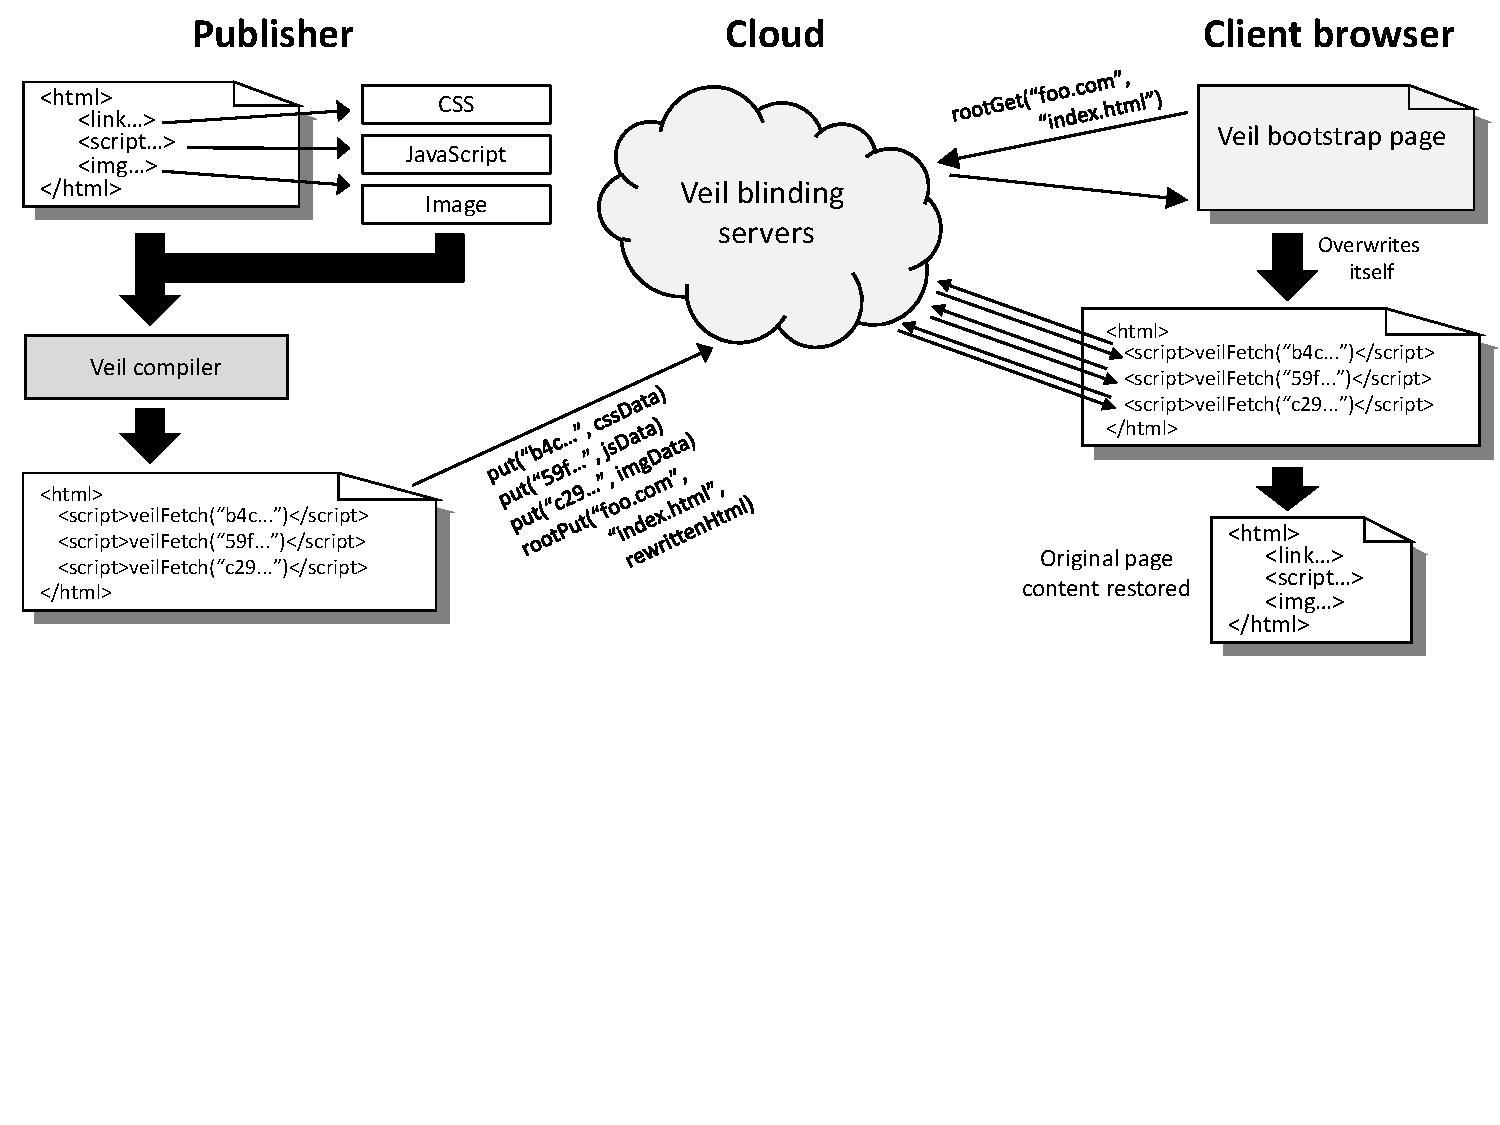
\includegraphics[width=\textwidth]{veil-figs/arch_small_cropped}
	\caption{The Veil architecture (cryptographic operations omitted for clarity).}
	\label{fig:arch}
\end{figure*}

As shown in Figure~\ref{fig:arch}, the Veil framework  %!!!jwm: Arg, the fig ref isn't resolving correctly.
consists of three components. The \emph{compiler}
transforms a normal web page into a new version
that implements static and dynamic privacy protections.
Web developers upload the compiler's output to
\emph{blinding servers}. These servers act as
intermediaries between content publishers and
content users, encrypting content. To load the Veil
page, a user first loads a small \emph{bootstrap page}.
The bootstrap asks for a per-user key and the
URL of the Veil page to load; the bootstrap then
downloads the appropriate objects from the blinding
servers and dynamically overwrites itself with
the privacy-preserving content in the target page.

In the remainder of this section, we describe Veil's
architecture in more detail. Our initial discussion
involves a simple, static web page that consists of
an HTML file, a CSS file, a JavaScript file, and an
image. We iteratively refine Veil's design to protect
against various kinds of privacy leakage. Then, we
describe how Veil handles more complex pages that
dynamically fetch and generate new content.


\subsubsection{The Veil Compiler and veilFetch()}
\label{sec:compiler}

The compiler processes the HTML in our example page (Figure~\ref{fig:arch}),
and finds references to three external objects (i.e.,
the CSS file, the JavaScript file, and the image).
The compiler computes a hash value for each object,
and then replaces the associated HTML tags with
dynamic JavaScript loaders for the objects. For
example, if the original image tag looked like this:
\begin{verbatim}
<img src="http://foo.com/img.jpg"/>
\end{verbatim}
the compiler would replace that tag with the following:
\begin{verbatim}
<script>veilFetch("b6a0d...");</script>
\end{verbatim}
where the argument to \texttt{veilFetch()} is the hash
name of the image. At page load time, when
\texttt{veilFetch()} runs, it uses an \texttt{XMLHttpRequest}
request to download the appropriate object from the
blinding service. In our example, the URL in the
\texttt{XMLHttpRequest} might be \texttt{http://veil.io/b6a0d...}.

Such a URL resides in the domain of the blinding
servers, not the domain of the original content
publisher. Furthermore, the URL identifies the underlying
object by hash, so the URL itself does not leak
information about the original publisher or the data
contained within the object. So, even though the
execution of \texttt{veilFetch()} may pollute
name-based interfaces like the DNS cache, a post-session
attacker which inspects those registries
cannot learn anything about the content that was fetched.
However, a network-observing attacker who sees a
\texttt{veilFetch()} URL can simply ask the blinding
server for the associated content, and then directly
inspect the data that the user accessed during the
private session!

To defend against such an attack, Veil associates
each user with a symmetric key $k_{user}$ (we describe
how this key is generated and stored in
Section~\ref{sec:bootstrap}). Veil also associates the
blinding service with a public/private keypair. When
\texttt{veilFetch(hashName)} executes, it does not
ask the blinding service for \texttt{hashName}---instead,
it asks for \texttt{<hashName>}$_{k_{user}}$. In the
HTTP header for the request, \texttt{veilFetch()} includes
$<k_{user}>_{PubKeyBServ}$, i.e., the user's symmetric
key encrypted by the blinding service's public key.
When the blinding service receives the request,
it uses its private key to decrypt $<k_{user}>_{PubKeyBServ}$.
Then, it uses $<k_{user}>$ to extract the hash
name of the requested object. The blinding service
locates the object, encrypts it with $k_{user}$,
and then sends the HTTP response back to the
client. Figure~\ref{fig:fetchProtocol} depicts
the full protocol.\footnote{%The protocol shown in
	%Figure~\ref{fig:fetchProtocol} requires a public
	%key operation for each request. However,
	A stateful blinding service can cache decrypted
	user keys and eliminate the public key operation
	from all but the user's first request.} In practice,
the blinding service's public/private
keypair can be the service's TLS keypair, as used
by HTTPS connections to the service. Thus, the
encryption of $k_{user}$ can be encrypted by the
standard TLS mechanisms used by an HTTPS connection.

Once \texttt{veilFetch()} receives the response,
it decrypts the data and then dynamically
reconstructs the appropriate object, replacing
the script tag that contained \texttt{veilFetch()}
with the reconstructed object. The compiler
represents each serialized object using JSON~\cite{json};
Figure~\ref{fig:imgJson} shows an example
of a serialized image. To reinflate
the image, \texttt{veilFetch()} extracts
metadata like the image's width and height,
and dynamically injects an image tag into
the page which has the appropriate attributes.
Then, \texttt{veilFetch()} extracts the
Base64-encoded image data from the JSON,
and sets the \texttt{src} attribute
of the image tag to a data URL~\cite{dataUrl}
which directly embeds the Base64 image
data. This causes the browser to load the
image. \texttt{veilFetch()} uses similar
techniques to reinflate other content types.

\begin{figure}
	\centering
	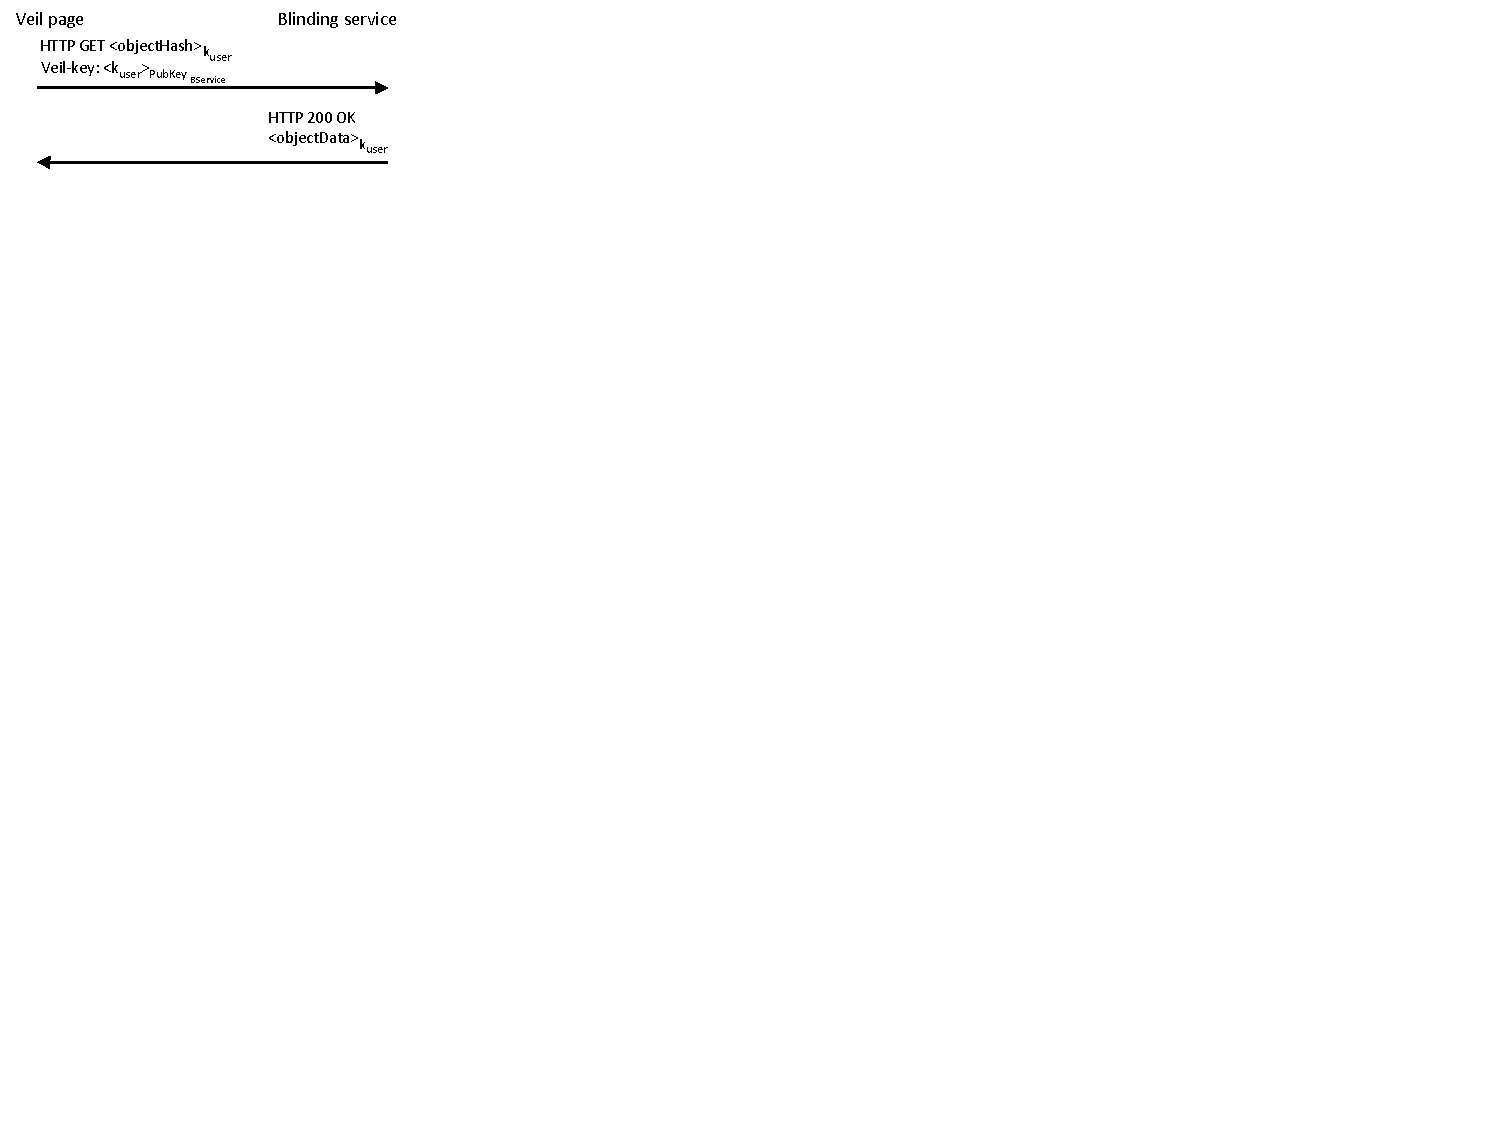
\includegraphics{veil-figs/fetchProtocol_cropped}
	\caption{The \texttt{veilFetch()} protocol.}
	\label{fig:fetchProtocol}
\end{figure}

\begin{center}
\begin{figure}
		\begin{BVerbatim}
		    {"img_type": "jpeg",
		    "dataURI": "ab52f...",
		    "tag_attrs": {"width": "20px",
		    "height": "50px"}}
		\end{BVerbatim}	
	\caption{A serialized \texttt{<img>} tag.}
	\label{fig:imgJson}
\end{figure}
\end{center}

This client-server protocol has several nice
properties. First, it solves the replay
problem---if an attacker wants to replay
old fetches, or guess visited URLs (as in a
CSS-based history attack~\cite{cssHistoryAttack,cssHistoryAttack2}),
the attacker will not be able to decrypt the
responses unless she has the user's key. Also,
since the blinding service returns encrypted
content, that encrypted content is what would
reside in the browser cache. Thus, Veil pages
can now persist data in the browser cache
such that only the user can decrypt and inspect
that content. Of course, a page does not have
to use the browser cache---when a publisher
uploads an object to the blinding service,
the publisher indicates the caching headers that the
service should return to clients.

In addition to uploading data objects like
images to the blinding service, the compiler
also uploads ``root'' objects. Root objects
are simply top-level HTML files like \texttt{foo.com/index.html}.
Root objects are signed with the publisher's
private key, and are stored in a separate
namespace from data objects using a 2-tuple
key that consists of the publisher name
(\texttt{foo.com}) and the HTML name
(\texttt{index.html}). Unlike data objects,
which are named by hash (and thus self-verifying),
root objects change over time as the associated
HTML evolves. Thus, root objects are
signed by the publisher to guarantee
authenticity and allow the blinding service
to reject fraudulent updates.


\subsubsection{The Blinding Service}
\label{sec:bservs}

In the previous section, we described the
high-level operation of the blinding service.
It exports a key/value interface to content
publishers, and an HTTP interface to browsers.
The HTTP code path does content encryption
as described above. As described in
Section~\ref{sec:mutation}, the blinding
service also performs \emph{content mutation}
to protect RAM artifacts that spill to disk;
mutation does not provide cryptographically
strong protections, but it does significantly
raise the difficulty of post-session forensics.
%We discuss specific mutation techniques in
%Section~\ref{sec:mutation}); for now, we note
%that mutation is a complement to heap walking
%(\S\ref{sec:heapWalk}), a separate technique
%which decreases the likelihood that RAM
%artifacts page out in the first place.
The blinding servers also implement the DOM
hiding protocol (\S\ref{sec:domHiding}), which
Veil sites can use to prevent exposing \emph{any}
site-specific HTML, CSS, or JavaScript to client
browsers.

%Content encryption allows Veil pages to
%securely persist state in the browser cache.
%However, this encryption cannot protect an
%application's in-memory data structures if those
%structures are reflected to disk, e.g., during
%paging, or when the system goes into hibernation
%mode and the OS takes a RAM snapshot. We assume
%that an attacker gains access to the user's machine
%after the private session has terminated, but
%operating systems frequently do not zero-out
%swap files and hibernation files. This allows
%forensic tools to find evidence of prior browsing
%sessions, \emph{even if those sessions used
%a native browser privacy mode}~\cite{aggarwal10,magnetForensicsChrome,ohana13}. 

%To make it more difficult for attackers to
%analyze memory artifacts, the blinding service
%\emph{mutates} the content that it returns to
%clients. Mutation generates objects that are
%structurally different from (but semantically
%%equivalent to) the canonical versions that
%were uploaded by the publisher. Content mutation
%ensures that, on different clients, each
%in-memory representation of an object is
%different. This prevents replay fingerprinting
%attacks in which the adversary loads a candidate
%private page on his own browser, extracts RAM
%artifacts, and then compares those artifacts
%to those that reside in the user's page file
%or hibernation file. As we describe below,
%mutation also makes it difficult for attackers
%to perform a first-principles analysis on memory
%images.

The blinding service can be implemented
in multiple ways, e.g., as a peer-to-peer
distributed hash table~\cite{pastry,chord},
a centralized service that is run by a
trusted authority like the EFF,
or even a single cloud VM that is paid for and
operated by a single privacy-conscious user. In
practice, we expect a blinding service to be run
by an altruistic organization like the EFF, or by
altruistic individuals (as in Tor~\cite{tor}),
or by a large set of privacy-preserving
sites who will collaboratively pay for the cloud
VMs that run the blinding servers. Throughout the
dissertation, we refer to a single blinding service
\texttt{veil.io} for convenience.
However, independent entities can simultaneously
run independent blinding services.

Veil's publisher-side protocol is compatible
with accounting, since the blinding service knows
which publisher uploaded each object, and how many
times that object has been downloaded by clients.
Thus, it is simple for a cloud-based blinding service
to implement proportional VM billing, or cost-per-download
billing. In contrast, an altruistic blinding service
(e.g., implemented atop a peer-to-peer DHT~\cite{pastry,chord})
could host anonymous object submissions for free.
%To minimize the client-perceived fetch latencies
%for blinded objects, the blinding servers should
%be widely distributed, similar to CDN nodes.

\subsubsection{The Same-origin Policy}
\label{sec:sop}

A single web page can aggregate content from a
variety of different origins. As currently
described, Veil maps all of these objects to
a single origin: at compile time, Veil downloads
the objects from their respective domains, and
at page load time, Veil serves all of the
objects from \texttt{https://veil.io}.

The browser uses the same-origin policy~\cite{sop}
to constrain the interactions between content
from different origins. Mapping all content to
a single origin would effectively disable
same-origin security checks. Thus, Veil's static
rewriter injects the \texttt{sandbox} attribute~\cite{iframeSandbox}
into all \texttt{<iframe>} tags. Using this
attribute, the rewriter forces the browser
to give each frame a unique origin with respect
to the same-origin policy. This means that,
even though all frames are served from the
\texttt{veil.io} domain, they cannot tamper
with each other's JavaScript state. In our current
implementation of the compiler, developers are
responsible for ensuring that dynamically-generated
frames are also tagged with the \texttt{sandbox}
attribute; however, using DOM virtualization~\cite{treehouse,mugshot},
the compiler could inject DOM interpositioning
code that automatically injects \texttt{sandbox}
attributes into dynamically-generated frames.

DOM storage~\cite{domStorage} exposes the
local disk to JavaScript code using a key/value
interface. DOM storage is partitioned by origin,
i.e., a frame can only access the DOM storage of
its own domain. By assigning an ephemeral, unique
origin to each frame, Veil seemingly prevents
an origin from reliably persisting data across
multiple user sessions of a Veil page. To solve
this problem, Veil uses indirection. When a
frame wants to access DOM storage, it first
creates a child frame which has the special URL
\texttt{https://veil.io/domStorage}. The child
frame provides Veil-mediated access to DOM storage,
accepting read and write requests from the parent
frame via \texttt{postMessage()}. Veil associates
a private storage area with a site's public key,
and engages in a challenge/response protocol
with a frame's content provider before agreeing
to handle the frame's IO requests; the challenge/response
traffic goes through the blinding servers (\S\ref{sec:dynamic}).
The Veil frame that manages DOM storage employs
the user's key to encrypt and
integrity-protect data before writing it,
ensuring that post-session attackers cannot
extract useful information from DOM storage
disk artifacts.

Since Veil assigns random, ephemeral origins
to frames, cookies do not work in the standard
way. To simulate persistent cookies, an origin
must read or write values in DOM storage. Sending
a cookie to a server also requires explicit
action. For example, a Veil page which contains
personalized content might use an initial piece
of non-personalized JavaScript to find the local
cookie and then generate a request for dynamic
content (\S\ref{sec:dynamic}).

\subsubsection{The Bootstrap Page}
\label{sec:bootstrap}
Before the user can visit any Veil sites, she
must perform a one-time initialization step
with the Veil bootstrap page (e.g., \texttt{https://veil.io}).
The bootstrap page generates a private symmetric key for
the user and places it in local DOM storage,
protecting it with a user-chosen password. Veil
protects the in-memory versions of the password and
symmetric key with heap walking (\S\ref{sec:heapWalk})
to prevent these cleartext secrets from paging to disk.

Later, the user determines the URL (e.g., \texttt{foo.com/index.html})
of a Veil site to load. The user should discover
this URL via an already-known Veil page like a
directory site, or via out-of-band mechanisms like a
traditional web search on a different machine than the
one needing protection against post-session attackers; looking
for Veil sites using a traditional search engine
on the target machine would pollute client-side state
with greppable content. Once the user possesses the
desired URL, she returns to the bootstrap page. The
bootstrap prompts the user for her password, extracts
her key from local storage, and decrypts it with the
password. The bootstrap then prompts the user for
the URL of the Veil page to visit. The bootstrap
fetches the root object for the page. Then, the
bootstrap overwrites itself with the HTML in the
root object. Remember that this HTML is the output
of the Veil compiler; thus, as the browser loads
the HTML, the page will use \texttt{veilFetch()}
to dynamically fetch and reinflate encrypted objects.

Once the bootstrap page overwrites itself, the user
will see the target page. However, no navigation will
have occurred, i.e., the browser's address bar will
still say \texttt{https://veil.io}. Thus,
the browser's history of visited pages will
never include the URL of a particular Veil page,
only the URL of the generic Veil bootstrap. The
compiler rewrites links within a page so that, if
the user clicks a link, the page will fetch the
relevant content via a blinded URL, and then deserialize
and evaluate that content as described above.

\subsubsection{Protecting RAM Artifacts}
\label{sec:heapWalk}

As a Veil page creates new JavaScript objects,
the browser transparently allocates physical
memory pages on behalf of the site. Later,
the OS may swap those pages to disk if memory
pressure is high and those pages are infrequently
used. JavaScript is a high-level, garbage-collected
language that does not expose raw memory addresses.
Thus, browsers do not define JavaScript interfaces
for pinning memory, and Veil has no explicit way
to prevent the OS from swapping sensitive data
to disk.

By frequently accessing sensitive JavaScript
objects, Veil \emph{can} ensure that the
underlying memory pages are less likely to be
selected by the OS's LRU replacement algorithm.
Veil's JavaScript runtime defines a \texttt{markAsSensitive(obj)}
method; using this method, an application indicates
that Veil should try to prevent \texttt{obj}
from paging to disk. Internally, Veil maintains
a list of all objects passed to \texttt{markAsSensitive()}.
A periodic timer walks this list, accessing every
property of each object using JavaScript reflection
interfaces. Optionally, \texttt{markAsSensitive()} can
recurse on each object property, and touch every
value in the object tree rooted by \texttt{obj}.
Such recursive traversals make it easier for
developers to mark large sets of objects at
once. JavaScript defines a special \texttt{window}
object that is an alias for the global namespace, so
if an application marks \texttt{window} as
recursively sensitive, Veil will periodically
traverse the entire heap graph that is reachable
from global variables. Using standard techniques
from garbage collection algorithms, Veil can
detect cycles in the graph and avoid infinite
loops.

\texttt{markAsSensitive()} maintains references
to all of the sensitive objects that it has ever
visited. This prevents the browser from garbage
collecting the memory and possibly reusing it
without applying secure deallocation~\cite{chow05}.
At page unload time, Veil walks the sensitive list
a final time, deleting all object properties.
Since JavaScript does not expose raw memory,
Veil cannot \texttt{memset()} the objects to
zero, but deleting the properties does make
it more difficult for a post-session attacker
to reconstruct object graphs.

Sensitive data can reside in the JavaScript
heap, but it can also reside in the memory
that belongs to the renderer. The renderer is
the browser component that parses HTML,
calculates the screen layout, and repaints
the visual display. For example, if a page
contains an HTML tag like \texttt{<b>Secret</b>},
the cleartext string \texttt{Secret} may
page out from the renderer's memory. As another
example, a rendered page's image content
may be sensitive.

The renderer is a C++ component that is
separate from the JavaScript engine;
JavaScript code has no way to directly
access renderer state. However, JavaScript
can indirectly touch renderer memory
through preexisting renderer interfaces.
For example, if the application creates
an empty, invisible \texttt{<img>} tag,
and injects the tag into the page's HTML,
the browser invalidates the page's layout.
If the application then reads the size
of the image tag's parent, the browser is
forced to recalculate the layout of the
parent tag. Recalculating the layout
touches renderer memory that is associated
with the parent tag (and possibly other
tags). Thus, Veil can walk the renderer
memory by periodically injecting invisible
tags throughout the HTML tree (forcing
a relayout) and then removing those
tags, restoring the original state of
the application.

The browser's network stack contains memory
buffers with potentially sensitive content
from the page. However, Veil only transmits
encrypted data over the network, so network
buffers reveal nothing to an attacker if
they page out to disk and are subsequently
recovered. Importantly, Veil performs
heap walking on the user's password and
symmetric key. This prevents those secrets
from paging out and allowing an attacker
to decrypt swapped out network buffers.

\subsubsection{Mutation Techniques}
\label{sec:mutation}
Veil's main protection mechanism for RAM
artifacts is heap walking, and we show in
Section~\ref{sec:privLeaks} that heap walking
is an effective defense during expected rates
of swapping. However, Veil provides a second
line of defense via content mutation. Mutation
ensures that, each time a client loads a page,
the page will return different HTML, CSS, and
JavaScript, even if the baseline version of the
page has not changed. Mutation makes grep-based
attacks more difficult, since the attacker
cannot simply navigate to a non-Veil version
of a page, extract identifying strings from the
page, and then grep local system state for those
strings. Content mutation is performed by the
blinding servers (\S\ref{sec:bservs}); below,
we briefly sketch some mutation techniques
that the blinding servers can employ.

Note that blinding servers can mutate content
in the background, \textit{before} the associated
pages are requested by a client. For example,
blinding servers can store a pool of mutated
versions for a single object, such that, when
a client fetches HTML that refers to the
object, the blinding server can late-bind
the mutated version that the page references.
Using this approach, mutation costs need not
be synchronous overheads that are paid when
a client requests a page. In addition, 
when a user requests a Veil page,
the blinding servers update the corresponding 
hashes for the mutated objects in the root object
before sending it to the user
to preserve the self-verification property of 
Veil objects described in Section~\ref{sec:compiler}. \\

\noindent
{\bf JavaScript:} To mutate JavaScript files, the
blinding service uses techniques that are adapted
from metamorphic viruses~\cite{hunting06}. Metamorphic
viruses attempt to elude malware scanners by
ensuring that each instantiation of the virus has
syntactically different code that preserves the
behavior of the base implementation. For example,
functions can be defined in different places, and
implemented using different sequences of assembler
instructions that result in the same output.

Our prototype blinding service mutates JavaScript code
using straightforward analogues of the transformations
described above. JavaScript code also has
a powerful advantage that assembly code
lacks---the \texttt{eval()} statement provides a
JavaScript program with the ability to emit new
mutated code at runtime. Such ``\texttt{eval()}-folding''
is difficult to analyze~\cite{zozzle}, particularly
if the attacker can only recover a partial set of
RAM artifacts for a page.\footnote{Some .NET viruses
	already leverage access to the runtime's reflection
	interface to dynamically emit code~\cite{szor05}.}

However, note that if a faulty blinding server forgets to mutate invocations
of \texttt{veilFetch(hashName)}, then unscrambled object
hash names may be paged out to disk in JavaScript source code! If an attacker
recovered such artifacts, he could directly replay the
object fetches that were made by the private session.
Thus, JavaScript mutation is a core responsibility for
the blinding service.\\

\noindent
{\bf HTML and CSS:} The grammars for HTML and CSS are
extremely complex and expressive. Thus, there are many
ways to represent a canonical piece of HTML or
CSS~\cite{webAppObfuscation}. For example, HTML allows %!!!Make sure I'm getting the details of this right.
a character to be encoded as a raw binary symbol in a
character encoding like \texttt{UTF-8} or \texttt{Unicode-16}.
HTML also allows characters to be expressed as escape
sequences known as HTML entities. An HTML entity consists
of the token ``\&\#'' followed by the Unicode code point
for a character and then a semicolon. For instance, the
HTML entity for ``a'' is ``\&\#97;''. The HTML
specification allows an HTML entity to have leading
zeroes which the browser ignores; the specification
also allows for code points to be expressed in
hexadecimal. Thus, to defeat simple exact-match
greps of HTML artifacts, the blinding service
can randomly replace native characters with random
HTML entity equivalents.

There are a variety of more sophisticated techniques
to obfuscate HTML and CSS. For a fuller exploration
of these topics, we defer the reader to other
work~\cite{webAppObfuscation}. Our blinding service
prototype uses random HTML entity mutation. It also
obscures the HTML structure of the page using
randomly inserted tags which do not affect the
user-perceived visual layout of the page.\\

\noindent
{\bf Images:} The blinding service can automatically
mutate images in several ways. For example, the
blinding service can select one of several formats
for a returned image (e.g., JPEG, PNG, GIF, etc.).
Each instantiation of the image can have a different
resolution, as well as different filters that are
applied to different parts of the visual spectrum.
Web developers can also use application-specific
knowledge to generate more aggressive mutations,
such as splitting a single base image into two
semi-transparent images that are stacked atop each
other by client-side JavaScript. %!!!Can you actually do this? :-)
As explained in our threat model (\S\ref{sec:threatModel}),
Veil does not protect against leaks of the raw
display bitmap that resides in GPU memory; thus,
the mutation techniques from above are sufficient
to thwart grep-based forensics on memory artifacts from
the DOM tree. For a more thorough discussion
of image mutation techniques that thwart
classification algorithms, we defer to literature
from the computer vision community~\cite{biggio11}.\\

% Orphan text that was removed from the intro.
% 
% To implement blinded references, Veil introduces a new
% set of \emph{blinding servers}. These servers sit between
% between users and application developers. Developers
% upload hash-named content to blinding servers, and users
% load a target page using Veil's bootstrap page, which
% gathers blinded objects via HTTP and uses them to
% dynamically reconstruct the target page. Blinding servers
% assist with mutating and encrypting content, but their
% clients can verify the integrity of blinded content
% using cryptography.
%
% From the perspective of a web browser, blinding servers
% export the standard HTTP interface and look like normal web
% servers. However, the blinding service can be implemented
% in multiple ways, e.g., as a distributed hash
% table~\cite{pastry,chord} or a centralized service run by
% a trusted authority. In practice, we expect that large
% groups of privacy-preserving sites will collaboratively
% pay for cloud VMs that run the blinding service
% (\S\ref{sec:bservs}). Blinding servers are compatible
% with per-publisher accounting mechanisms, so Veil can
% track how much traffic is associated with each Veil
% site and implement proportional VM billing.


% !!!Do we want to mention this?
% Metamorphic content and Veil strings also allow
% us to thwart forensics which looks at browser memory
% consumption to fingerprint pages~\cite{memento}.

\subsubsection{Dynamic Content}
\label{sec:dynamic}

At first glance, Veil's compile-time binding of
URLs to objects seems to prevent a publisher
from dynamically generating personalized user
content. However, Veil can support dynamic
content generation by using the blinding
service as a proxy that sits between the
end-user and the publisher. More specifically,
a Veil page can issue an HTTP request with
a \texttt{msg-type} of ``forward''. The body
of the request contains two things: user information
like a site-specific Veil cookie (\S\ref{sec:sop}),
and a publisher name (e.g., \texttt{foo.com}).
The page gives the request a random hash name,
since the page will not cache the response.
When the blinding service receives the request,
it forwards the message to the publisher's
dynamic content server. The publisher generates
the dynamic content from the provided user
information, and then sends the content to the
blinding service, who forwards it to the client
as the HTTP response to the client's ``forward''
request. The client and the publisher can encrypt
the user information and the personalized content
if the blinding service is not trusted with
user-specific data; in this scenario, the content provider's web server
is responsible for mutating objects before returning
them to the client. Regardless, the content provider
must compile dynamically-generated content (\S\ref{sec:compiler}
and \S\ref{sec:porting}).

Another option is to start with the same forwarding
protocol as above, but instead of having
the publisher compile and mutate the content, the 
publisher just sends the unmodified user-specific
content back to the blinding servers. Then, the blinding
servers compile and mutate the content before
returning it to the user. 

The question is which of the two options is better. 
More specifically, should the blinding servers
or the publishers perform compilation and mutation?
Ideally, the end host
would manipulate the dynamic content as it might
contain sensitive user information, which can be 
encrypted on host and thus hidden from the blinding servers.
However, the downside is that all end hosts have to 
adopt Veil. Having the proxy perform the manipulation
solves this problem, but this scenario would
require the proxy to handle a heavier computation workload.
The networking community
has examined these tradeoffs in a similar context, 
so we refer the reader to that specific research for a more in-depth
discussion~\cite{flywheel,polaris}.
The performance overhead is minimal because only the dynamic
portions of the site have to be compiled during the page load, 
and more detailed numbers are in Section~\ref{sec:macrobench}.

\subsubsection{DOM Hiding}
\label{sec:domHiding}

Heap walking reduces the likelihood that in-memory browser
state will swap to disk. Content mutation ensures that, if
state does swap out, then the state will not contain greppable
artifacts from a canonical version of the associated page.
However, some Veil sites will be uncomfortable with sending
\emph{any} site-specific HTML, CSS, or JavaScript to a client,
even if that content is mutated. For example, a site might
be concerned that a determined sysadmin can inspect swapped-out
fragments of mutated HTML, and try to reverse-engineer the
mutation by hand.

To support these kinds of sites, Veil provides a mode of
operation called DOM hiding. In DOM hiding mode, the user's
browser essentially acts as a thin client, with the full
version of the page loaded on a remote server that belongs
to the content provider. The user's browser employs a generic,
page-agnostic JavaScript library to forward GUI events to
the content provider through the blinding service; the content
provider's machine applies each GUI event to the server-side
page, and then returns an image that represents the new state
of the page.

The advantage of DOM hiding is that site-specific HTML, CSS,
and JavaScript is never pushed to the user's browser. The
disadvantage is that each GUI interaction now suffers from
a synchronous wide-area latency. For some Veil sites,
this trade-off will be acceptable. We characterize the
additional interactive latency in Section~\ref{sec:dhEval}.

\begin{figure}
	\centering
	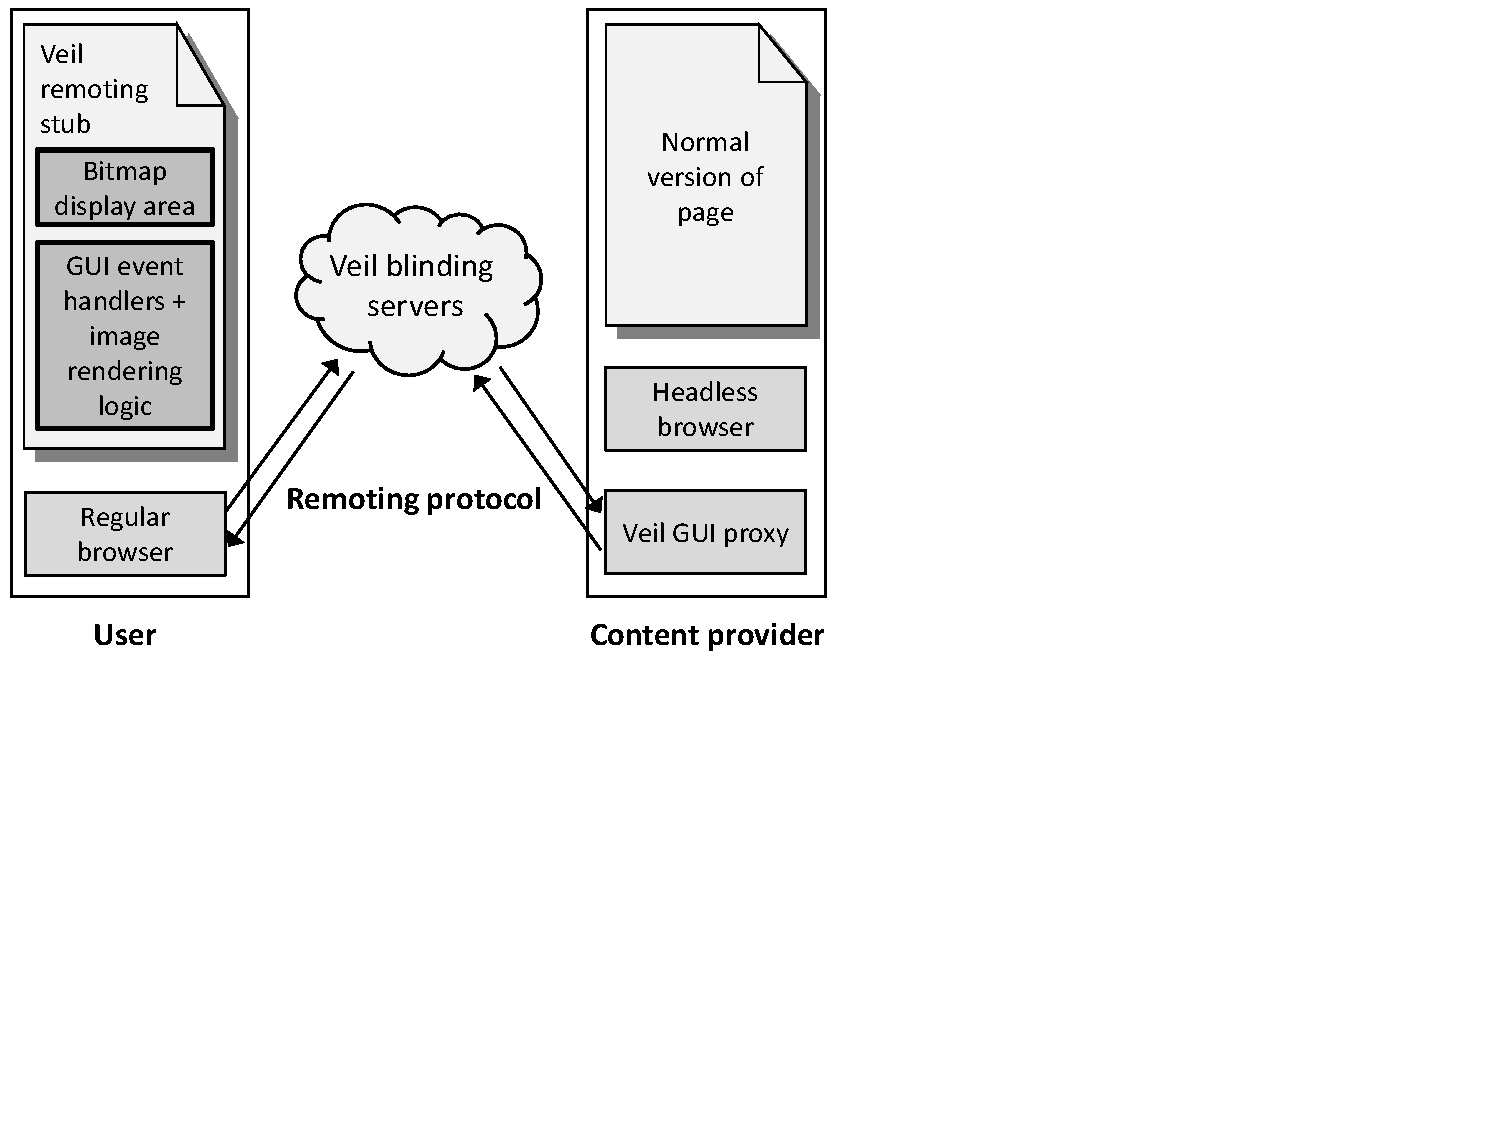
\includegraphics[width=\textwidth]{veil-figs/domHiding.pdf}
	\caption[Overview of DOM hiding mode]{With DOM hiding, the client-side remoting stub sends
		GUI events to the content provider, and receives bitmaps
		representing new page states. The page's raw HTML, CSS,
		and JavaScript are never exposed to the client.}
	\label{fig:domHiding}
\end{figure}

Figure~\ref{fig:domHiding} provides more details about how Veil
implements DOM hiding. The Veil bootstrap page receives the
URL to load from the user, as described in Section~\ref{sec:bootstrap}.
The bootstrap page then issues an initial HTTP request through
the blinding servers to the content provider.
The content provider returns a page-agnostic remoting stub;
this stub merely implements the client-side of the remote
GUI architecture. As the content provider returns the stub
to the user, the provider also launches a headless browser\footnote{A
	headless browser is one that does not have a GUI. However, a
	headless browser \emph{does} maintain the rest of the browser
	state; for example, DOM state can be queried using normal DOM
	methods, and modified through the generation of synthetic DOM
	events like mouse clicks.} like PhantomJS~\cite{phantomJS} to load
the normal (i.e., non-rewritten) version of the page. The
content provider associates the headless browser with a Veil
GUI proxy. The proxy uses native functionality in the headless
browser to take an initial screenshot of the page. The GUI
proxy then sends the initial screenshot via the blinding servers
to the user's remoting stub. The stub renders the image, and
uses page-agnostic JavaScript event handlers to detect
GUI interactions like mouse clicks and keyboard presses. 
The stub forwards those events to the GUI
proxy. The proxy replays those events in the headless
browser, and ships the resulting screen images back to the
client. Note that a page which uses DOM hiding will not
use encrypted client-side browser caching (\S\ref{sec:compiler})
or DOM storage (\S\ref{sec:sop})---there
will be no page-specific client-side state to store.

\subsubsection{Discussion}
\label{sec:discussion}

Veil tries to eliminate cleartext client-side
evidence of browsing activity. However, Veil does
not prevent the server-side of a web page from
tracking user information. Thus, Veil is compatible
with preexisting workflows for ad generation and
accounting (although advertising infrastructure
must be modified to use blinded URLs and
``forward'' messages).

% jwm: Hmm, on second read, this paragraph doesn't
%      seem very enlightening . . .
%
% Like all programs that perform cryptography, a Veil
% page is forced to store sensitive keys in cleartext
% form at certain points during execution. For example,
% the Veil page must load the cleartext user password into
% memory before it can decrypt the user's symmetric key;
% later, the page must use that cleartext symmetric key
% to decrypt objects that are returned by the blinding
% service. If an attacker can recover such material from
% a RAM artifact, it makes it easier to analyze other
% data that may have leaked from the private session
% (although content mutation will still present the
% attacker with challenges). The necessity for cleartext
% cryptographic keys is problematic, but it seems
% intrinsic to any program that performs cryptography.

If a Veil page wants to use the browser cache, Veil
employs encryption to prevent attackers from inspecting
or modifying cache objects. However, an attacker may
be able to fingerprint the site by observing the size
and number of its cached objects. Sun et al.~\cite{sun02} provide a
survey of techniques which prevent such fingerprinting attacks; 
their discussion is in the context of
protecting HTTPS sessions, but their defensive
techniques are equally applicable to Veil. The strongest
defense is to reduce the number of objects in a page.
Veil's compiler can easily do this by inlining objects
into HTML~\cite{silo}; for example, the compiler can
directly embed CSS content that the original HTML
incorporated via a link to an external file. The blinding
service can also inject noise into the distribution of object
sizes and counts. For example, when the service returns
objects to clients, it can pad data sizes to fixed offsets,
e.g., 2KB boundaries or power-of-2 boundaries. Alternatively,
the blinding service can map object sizes for page $X$ to
the distribution for object sizes in a different page
$Y$~\cite{wright09}. All of these defensive approaches
hurt performance in some way---inlining and merging
reduce object cacheability, and padding increases the
amount of data which must be encrypted and transmitted
over the network. Note that publishers must explicitly
enable client-side caching, so paranoid sites can simply
disable this feature.

%A private web service can inadvertently leak information
%about its user base via server-side timing channels
%~\cite{serverTimingAttacks}. For example, suppose that
%a service's login page requires a user to enter an
%email address. Further suppose that, on the web server,
%processing a login with a valid email address takes
%a different amount of time than processing a login
%that uses an invalid address. If an attacker knows a
%user's email address, he can reveal whether the user
%has visited the private site by navigating to the site
%himself, performing two login attempts (one with the
%user's real email address, and another with a fake
%email address), and observing whether the server-side
%timing is the same. Veil does not specifically address
%this attack, but Veil is compatible with solutions
%like the \texttt{mod\_timepad} Apache module~\cite{serverTimingAttacks}.

\subsection{Porting Legacy Applications}
\label{sec:porting}

In this section, we describe how Veil helps developers
to port legacy web pages to the Veil framework. In
particular, we provide case studies which demonstrate
how Veil's compiler and runtime library can identify
unblinded fetches and, in some cases, automatically
transform those fetches into blinded ones.\\

\noindent
{\bf Raw XMLHttpRequests:} Veil's compiler traverses
a statically defined HTML tree, converting raw URLs
into Veil hash pointers. However, a page's JavaScript
code can use \texttt{XMLHttpRequests} to dynamically
fetch new content. Veil's static HTML compiler does
not interpose on such fetches, so they will generate
unblinded transfers that pollute the client's DNS cache
and browser cache.

In debugging mode, Veil's client library shims the
JavaScript runtime~\cite{mugshot} and interposes on
the \texttt{XMLHttpRequest} interface. This allows
Veil to inspect the URLs in \texttt{XMLHttpRequests}
before the associated HTTP fetches are sent over the
network. Veil drops unblinded requests and writes the
associated URLs to a log. A web developer can then
examine this log and determine how to port the URLs.

For static content, one porting solution is to leverage
Veil's \textit{AJAX maps}. Once the debugging client
library has identified a page's raw \texttt{XMLHttpRequest}
URLs, the library sends those URLs to Veil's HTML
compiler. The compiler automatically fetches the associated
objects and uploads them to the object servers. Additionally,
when the compiler rewrites the HTML, it injects
JavaScript code at the beginning of the HTML which maps
the raw \texttt{XMLHttpRequest} URLs to the hash names
of the associated objects. Later, when the page is
executed by real users, Veil's shimmed \texttt{XMLHttpRequests}
use the AJAX map to convert raw URLs to blinded references.
Veil will drop requests that are not mentioned in
the translation map. This approach is complete from
the security perspective, since all unblinded \texttt{XMLHttpRequests}
will be dropped. However, for this approach to please users
(who do not want \textit{any} requests to drop),
Veil developers should use testing tools with good
coverage~\cite{monkeytest,clickmonkey,sahi} to ensure
that all of a page's \texttt{XMLHttpRequest} URLs are
mapped.

AJAX maps are unnecessary for native Veil pages
which always generate blinded \texttt{XMLHttpRequests}.
However, URL validation via \texttt{XMLHttpRequest}
shimming is useful when developers must deal with
complex legacy libraries.\\

\noindent
{\bf Dynamic tag generation:} A legacy page can generate
unblinded fetches by dynamically creating new DOM nodes
that contain raw URLs in \texttt{src} attributes. For
example, using \texttt{document.createElement()}, a page
can inject a new \texttt{<img>} tag into its HTML\@. A
page can also write to the \texttt{innerHTML} property
of a preexisting DOM node, creating a new HTML subtree
that is attached to the preexisting node. Neither type of
tag creation will be captured by \texttt{XMLHttpRequest}
shimming.

\texttt{XMLHttpRequest} shimming is a specific example
of a more general technique called DOM virtualization.
If desired, the entire DOM interface can be
virtualized~\cite{psj,treehouse,jigsaw}, allowing Veil to interpose
on all mechanisms for dynamic tag creation. However,
full DOM virtualization adds non-trivial performance
overhead---the native DOM implementation is provided by
the browser in fast C++ code, but a virtualized DOM is
implemented by the application in comparatively slow JavaScript
code. Furthermore, the full DOM interface is much more
complex than the narrow \texttt{XMLHttpRequest} interface. 

Our current implementation of Veil supports
\texttt{XMLHttpRequest} shimming, but not full DOM
virtualization. We leave the integration of Veil with
a full virtualization system~\cite{treehouseGit} as
future work.\\

\noindent
{\bf Unblinded links in CSS:} CSS files can directly
reference image objects using the \texttt{url()}
statement, e.g., \texttt{body\{background: url(`x.jpg')\}}.
After the Veil compiler processes HTML files, it
examines the associated CSS files and replaces raw
image links with inline data URLs. Thus, when the
Veil page loads a post-processed CSS file, the image
data will be contained within the CSS itself, and will
not require network fetches.\\

\noindent
{\bf Angular.js:} Angular~\cite{angular} is a popular
JavaScript framework that provides model-view-controller
semantics for web applications. Angular uses a
declarative model to express data bindings. For
example, the \texttt{\{\{\}\}} operator is used to embed
live views of the controller into HTML\@. The HTML
snippet \texttt{<img src=\{\{controller.x\}\}/>} instructs
Angular to dynamically update the content of the
\texttt{<img>} whenever the JavaScript value
\texttt{controller.x} changes. Many other popular
frameworks define a similar templating mechanism~\cite{backbone,kendo,ember}.

The \texttt{\{\{\}\}} operator is not part of the official
HTML grammar. To implement \texttt{\{\{\}\}} and other
kinds of data binding, Angular uses a dynamic DOM
node compiler. This compiler is a JavaScript file
that runs at the end of the page load, when the initial DOM
tree has been assembled. The compiler locates special
Angular directives like \texttt{\{\{\}\}}, and replaces
them with new JavaScript code and DOM nodes
that implement the data binding protocol.

Angular allows URLs to contain embedded \texttt{\{\{\}\}}
expressions. Since these URLs are not resolved until
runtime, Veil's static compiler cannot directly
replace those URLs with blinded ones. However, Veil
can rewrite Angular directives in a way that passes
control to Veil code whenever a data binding changes.
In the previous \texttt{<img>} example, Veil rewrites
the tag as follows:

\begin{verbatim}
<img src="0" alt={{controller.x}}/>
\end{verbatim}
The \texttt{src} attribute of the image is set to
a network path which is known to be nonexistent
(but whose URL does not leak private information).
When the page tries to load the image, the load
failure will invoke a custom \texttt{onerror}
handler that Veil has attached to the \texttt{window}
object. That handler will read the value of the
\texttt{alt} attribute, which will contain the
dynamic value of \texttt{controller.x}. Veil
will then issue a blinded fetch for the associated
image. In parallel, Veil also sets an Angular
\texttt{\$watch()} statement to detect future
changes in \texttt{\{\{controller.x\}\}}; when a
change occurs, Veil reads the new value, and then
blindly fetches and updates the image as before.
This basic approach is compatible with the template
semantics of other popular JavaScript
frameworks~\cite{backbone,kendo,ember}.

If dynamic Angular URLs can be drawn from an arbitrarily
large set, Veil uses the ``forward'' message type
from Section~\ref{sec:discussion} to bind the
raw URL to a blinded one. If the URL is drawn
from a finite set, the compiler can upload the
associated objects to the blinding service,
and then inject the page with a blinding
map that translates resolved Angular URLs
to the associated hash names. The blinding
service mutates that table in the same way
that it mutates the hash names passed to
\texttt{veilFetch()}.

\subsection{Implementation}
\label{sec:impl}

Our Veil prototype consists of a compiler,
a blinding server, a GUI proxy, a bootstrap page,
and a client-side JavaScript library that
implements \texttt{veilFetch{}()}
%, the \texttt{v\_str} object,
and other parts of the Veil runtime.

We implemented the compiler and the blinding
server in Python. The compiler uses
BeautifulSoup~\cite{beautifulSoup} to
parse and mutate HTML; the compiler also
uses the Esprima/Escodegen tool chain~\cite{esprima,escodegen}
to transform JavaScript code into ASTs, and
to transform the mutated ASTs back into
JavaScript. To implement cryptography, we use the
PyCrypto library~\cite{pyCrypto}
in the blinding server, and the native
Chrome WebCrypto API~\cite{webCrypto} 
in the Veil JavaScript library. We 
use OpenCV~\cite{opencv} to perform
image mutation on the blinding server.

To implement DOM hiding, we used Chrome 
running in headless mode as the browser
used by the content provider's GUI proxy.
The GUI proxy was written in Python, and
used Selenium~\cite{selenium} to take
screenshots and generate synthetic GUI
events within the headless browser.

\subsection{Evaluation}
\label{sec:eval}

In this section, we evaluate Veil's raw
performance, and its ability to safeguard
user privacy. Using forensic tools and
manual analysis, we find that blinded
references and encrypted objects are
sufficient to prevent information leakage
through the browser cache and name-based
interfaces like the DNS cache. We show
that Veil's heap walking techniques are
effective at preventing secrets from paging
out unless system-wide memory pressure is
very high. We also demonstrate that the performance
of our Veil's prototype is acceptable, with
page load slowdowns of 1.2x--3.25x.

\begin{figure*}
	\centering
	\begin{tabular}{lr}
		\toprule
		\bf Operation & \bf Speed \\
		\midrule
		Generate an AES key and encrypt it with RSA public key (2048 bit)  & 0.75 ms \\
		% Throughtput for verifying 2048 bit RSA PKCS 1 signature on index file & 215 MB/s \\
		Encrypt 64 character hash (blinded reference) & 0.16 ms \\
		Throughput for decryption using AES-CTR & 520 MB/s \\
		Throughput for verifying SHA256 hash of file & 220 MB/s \\
		\bottomrule
	\end{tabular}
	\caption{Overhead for client-side JavaScript cryptography using the WebCrypto API~\cite{webCrypto}.}
	\label{fig:cryptoCost}
\end{figure*}

All performance tests ran on a machine with
a 2 GHz Intel Core i7 CPU with 8GB of RAM.
Unless otherwise specified, those tests ran in
the Chrome browser, and we ran each experiment
100 times and measured the average. We configured
Veil to use 2048-bit RSA and 128-bit AES in CTR
mode. The phrase ``standard Veil mode''
corresponds to non-DOM hiding mode.

\subsubsection{Performance Microbenchmarks}
\label{sec:microbench}

Veil uses cryptography to implement blind references
and protect the data that it places in client-side storage.
Figure~\ref{fig:cryptoCost} depicts the costs %!!!jwm: For some reason, doing a ~\ref{fig:cryptoCost} doesn't work!
for those operations. Before a user can load a Veil
page, she must generate an AES key and encrypt it
with the blinding service's RSA key. This one time
cost is 0.75 ms. The remaining three rows in Figure~\ref{fig:cryptoCost}
depict cryptographic %!!!jwm: For some reason, doing a ~\ref{fig:cryptoCost} doesn't work!
overheads that Veil incurs during a page load.
\begin{itemize}
	%    \item After the bootstrap page downloads a
	%          top-level HTML file, the bootstrapper
	%          must verify that the file is signed by
	%          the publisher. This operation proceeds
	%          at 215 MB/s; so, for an 100 KB HTML file,
	%          Veil would require 0.5 ms to validate
	%          the signature.
	\item For \texttt{veilFetch()} to generate a
	blinded reference, it must encrypt a
	hash value with the user's AES key. This
	operation took 0.16 ms.
	\item When \texttt{veilFetch()} receives a
	response, it must decrypt that response
	with the AES key. That operation proceeds
	at 520 MB/s. For example, decrypting a
	300 KB image would require 0.6 ms.
	\item \texttt{veilFetch()} also validates the
	hash of the downloaded object. This
	proceeds at 220 MB/s, requiring 1.3 ms
	for a 300 KB image.
\end{itemize}
Figure~\ref{fig:cryptoCostServer} depicts the
cryptography overheads on the server-side of
the protocol. End-to-end, fetching a 300 KB
object incurs roughly 10 ms of cryptographic
overhead. 

\begin{figure}
	\centering
	\begin{tabular}{lr}
		\toprule
		\bf Operation & \bf Speed \\
		\midrule
		Decrypt AES key (2048 bit RSA)  & \phantom{0}3.1 ms \\
		Decrypt 64 char hash (blinded reference) & 0.04 ms \\
		Throughput for encryption using AES-CTR & 62 MB/s \\
		\bottomrule
	\end{tabular}
	\caption{Overhead for server-side operations using PyCrypto~\cite{pyCrypto}.}
	\label{fig:cryptoCostServer}
\end{figure}

\subsubsection{Performance Macrobenchmarks: Standard Veil Mode}
\label{sec:macrobench}

To measure the increase in page load
time that Veil imposes, we ported six sites
to the Veil framework.  \textbf{Washington Post}
is the biggest site that we ported, and contains
large amounts of text, images, and JavaScript
files. \textbf{Imgur} is a popular image-sharing
site; compared to the other test sites, it has
many images but less text. \textbf{Woot!} is an
e-commerce site that has a large amount of text
and images, but comparatively few scripts.
\textbf{Piechopper} is a highly dynamic site that
uses Angular (\S\ref{sec:porting}). Piechopper is
script-and-text heavy, but has few images.
\textbf{University} represents a university's
website. This site is the smallest
one that we tested, although it uses CSS with raw
URLs that Veil must blind (\S\ref{sec:porting}).
\textbf{Google} represents the results page for
the search term ``javascript.''  Most of that page's
JavaScript and CSS objects are inlined into
the HTML, meaning that they do not require
network fetches. 

To port a preexisting site to Veil, we had the
compiler download the top-level HTML file and
extract the URLs which referenced external objects like
images. The compiler downloaded those objects from
the relevant servers. After calculating hashes
for those objects (and converting raw URLs into
blinded ones), the compiler uploaded the objects
to the blinding server. Since preexisting sites
were not designed with Veil in mind, they
occasionally fetched content dynamically, e.g.,
via unblinded \texttt{<img>} tags generated by
JavaScript at runtime. For sites like this, we
observed which objects were dynamically fetched,
and then manually handed them to the compiler
for processing; we also manually rewrote the
object fetch code to refer to the compiler-generated
object names. Native Veil pages would invoke
the Veil runtime library to dynamically fetch
such content, avoiding the need for manual
rewriting. \\

\begin{figure}
	\centering
	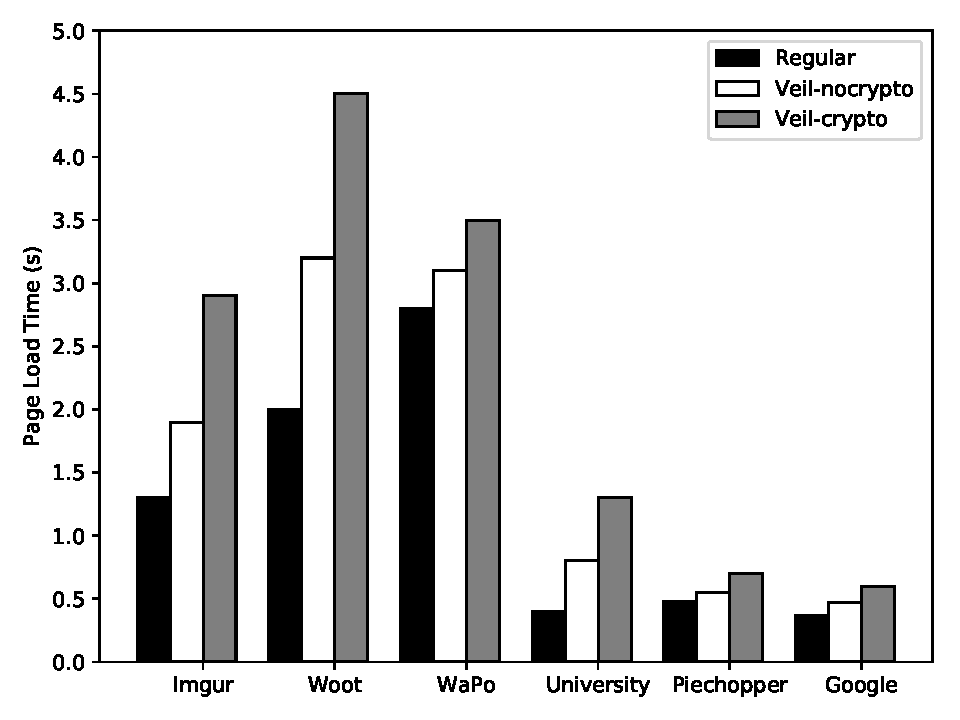
\includegraphics[width=\textwidth]{veil-figs/perf_graph.pdf}
	\caption{Page load times for each website: regular; with Veil (but no cryptography); with Veil (and using cryptography).}
	\label{fig:loadTime}
\end{figure}

\noindent
\textbf{Page load time:}
Figure~\ref{fig:loadTime} depicts the load times
for three versions of each site: the regular version
of the site, a Veil port that does not perform
cryptography, and a Veil port with cryptography
enabled. The regular versions of a page were loaded
from a localhost webserver, whereas the Veil pages
were loaded from a localhost blinding server. This setup
isolated the overhead of cryptography and content
mutation.

As shown in Figure~\ref{fig:loadTime}, page loads using Veil with
no cryptography were 1.25x--2x slower. This is mostly
due to extra computational overhead on the client.
For example, parsing overheads increased because,
as we quantify below, mutated objects were larger than
the baseline objects; for images, the browser also
had to Base64-decode the bitmaps before displaying
them.
%jwm: The below is no longer true, since we've
%     made the jump to asynchronous WebCrypto.
%Also note that \texttt{veilFetch()} downloads
%content synchronously, and that script tags
%halt the parsing process; since Veil replaces
%all image and CSS tags with script tags, this
%limits the browser's ability to continue parsing
%while previously visited tags are loading their
%content.
Veil with cryptography added another slowdown factor
of 1.1x--1.63x, with higher penalties for pages
with many objects (regardless of their type). The
end-to-end slowdown for the full Veil system
was 1.25x--3.25x. Note that these slowdowns were for
browsers with cold caches; 
Veil's overhead would
decrease with caching, since server-side
cryptography could be avoided. Also note that
the University site was a challenging case for
Veil, because the site was small in absolute size,
but has many small images. Thus,
Veil's per-blinded-reference cryptographic
overheads (see Figures~\ref{fig:cryptoCost} and~\ref{fig:cryptoCostServer}) %!!!jwm: See above re: broken fig command.
were paid more frequently. A Veil-optimized
version of the site would use image spriting~\cite{spriting}
to combine multiple small images into a single,
larger one.\\

\noindent
\textbf{Dynamic content overhead:}
As described in Section~\ref{sec:dynamic},
dynamic content has some overhead because it
has to be compiled during the page load.
Fortunately, the compilation cost for a single dynamic object
is typically small. For example, compiling a
100 KB image requires Base64-encoding it and
generating a few metadata fields, taking roughly
75 ms. Content providers or blinding servers 
can compile multiple dynamic objects in parallel. \\

\begin{figure}
	\centering
	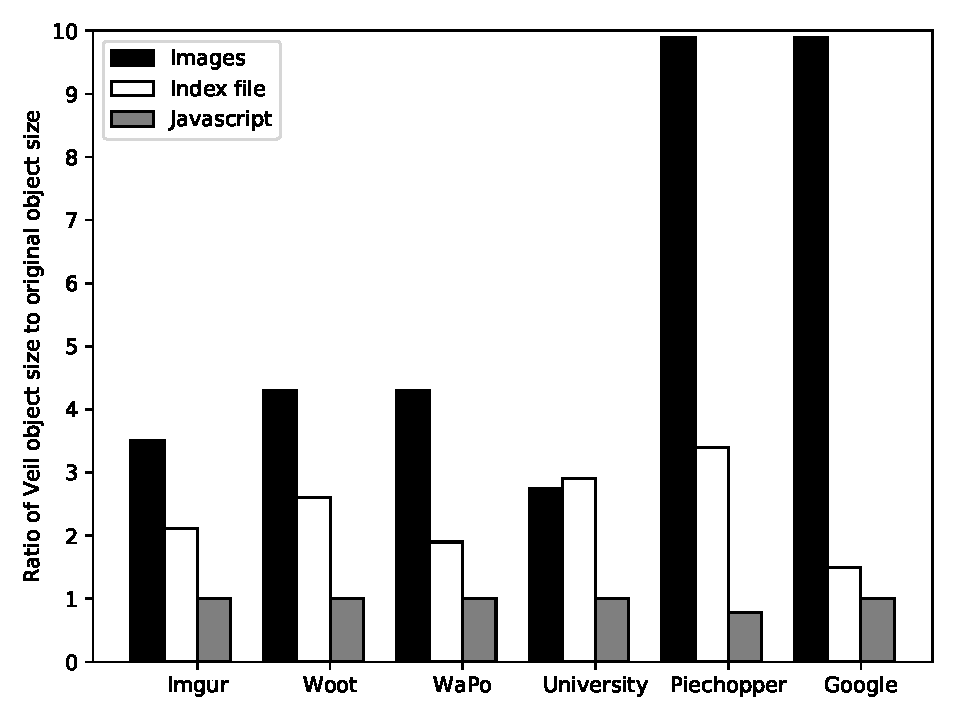
\includegraphics[width=\textwidth]{veil-figs/size_graph.pdf}
	\caption{Size increases for Veil's mutated objects.}
	\label{fig:mutateSize}
\end{figure}

\noindent
\textbf{Object growth:}
Figure~\ref{fig:mutateSize} shows how object sizes grew
after post-processing by Veil. Images experienced
two sources of size expansion: mutation and Base64
encoding. Base64 encoding resulted in a 1.33x size
increase. Our Veil prototype implements mutation via
the addition of Gaussian noise, with the resulting
size increases dependent on the image format. PNG
is lossless, so the addition of noise generated
a 10x size increase. In contrast, JPG is a lossy
format, so noise injection resulted in less than
a 2x size increase. The Piechopper and Google pages
contained many PNGs, and thus suffered from worse
image expansion than the other test pages.

As shown in Figure~\ref{fig:mutateSize}, mutated
JavaScript files typically remained the same size,
or became somewhat smaller---mutation adds source
code, but Veil passes the mutated code through
a minifier which removes extraneous whitespace
and rewrites variable names to be shorter. HTML
suffered from larger size increases, because
mutation tricks like random HTML entity encoding
strictly increase the number of characters in the
HTML. \\

\begin{figure}
	\centering
	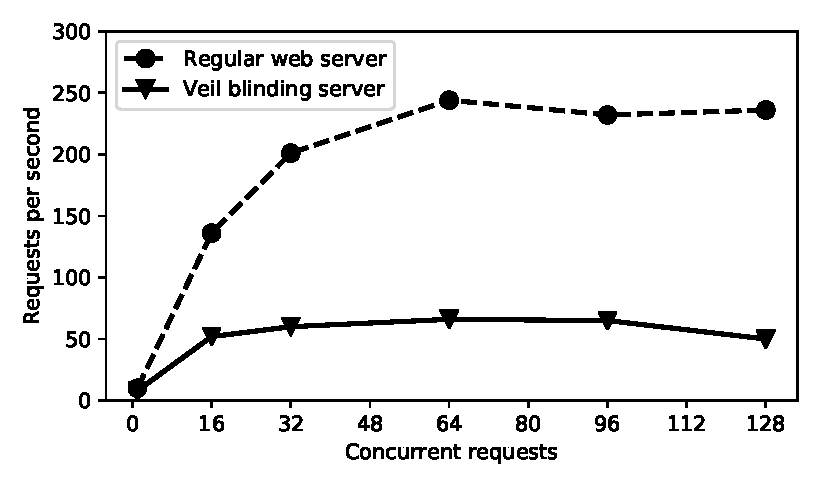
\includegraphics[width=\textwidth]{veil-figs/scalability_mit.pdf}
	\caption{Scalability comparison between a blinding server
		and a regular web server.}
	\label{fig:scalability}
\end{figure}

\noindent
\textbf{Server-side scalability:}
Figure~\ref{fig:scalability} shows the HTTP-level
request throughput of a Veil blinding server,
compared to the baseline performance of a blinding
server that performed none of Veil's added functionality
(and thus acted as a normal web server).
% The client and the servers were on the same machine, but
% client/server traffic used an emulated link
% with 25 ms latency and 500 Mbit/s of download
% bandwidth, to roughly simulate the public-facing
% network connection available to a blinding server
% run on an EC2 \texttt{c4.large} VM~\cite{!!!}. %  https://cloudspectator.com/wp-content/uploads/report/iaas_generational_aws_c3_c4.compressed.pdf
% Network emulation was performed using PF and dummynet.
HTTP requests were generated using \texttt{ab}, the Apache
benchmarking tool~\cite{ab}.

As shown in Figure~\ref{fig:scalability}, Veil
reduces web server throughput by roughly 70\%
due to the additional cryptographic operations
that Veil must perform. By quantifying 
Veil's scalability penalty for a fixed client load
compared to a regular web
server, blinding server hosts 
can know the additional servers needed 
to handle a specific load on a Veil page.
Remember that when
Veil operates in regular (i.e., non-DOM hiding
mode), Veil blinding servers mutate content in
the background, out of the critical path for an
HTTP response; thus, the slowdowns in Figure~\ref{fig:scalability}
are solely caused by synchronous cryptographic
operations. \\

\subsubsection{Preventing Information Leakage}
\label{sec:privLeaks}


{\bf Name-based interfaces:} To determine
how well Veil protects user privacy, we created
a baseline VM image which ran Lubuntu 13.10 and
had two different browsers (Firefox and Chrome). In
the baseline image, the browsers were installed, but they had
not been used to visit any web pages. We then ran
a series of experiments in which we loaded the
baseline image, opened a browser, and then visited
a single site. We took a snapshot of the browser's
memory image using \texttt{gcore}, and we also
examined disk state such as the browser
cache and the log entries for DNS resolution
requests. We did this for the regular and
Veil-enabled versions of each page described in
Section~\ref{sec:macrobench}.

In all tests, the Veil pages were configured to
store data in the browser cache, and in all tests,
the cache only contained encrypted data at the
end of the private session. Greps through the
memory snapshots and DNS records did not reveal
cleartext URLs or hostnames. Unsurprisingly,
the regular versions of the web pages left
unencrypted data in the browser cache, and
various cleartext URLs in name-based data
stores. To cross-validate these results, we
repeated these experiments on Windows, and used
the Mandiant Redline forensics tool~\cite{mandiant}
to search for post-session artifacts in persistent
storage. Redline confirmed that the only
cleartext URL in the browser history was the
URL for the Veil bootstrap page, and that all
other URLs were blinded.
%jwm: Maybe restore for camera-ready? Or not.
% Note that visiting a Veil page does not add
% a new entry to the browser's ``visited pages''
% history, because the bootstrap page overwrites
% itself without changing the URL in the address bar.
\\

\begin{figure}
	\centering
	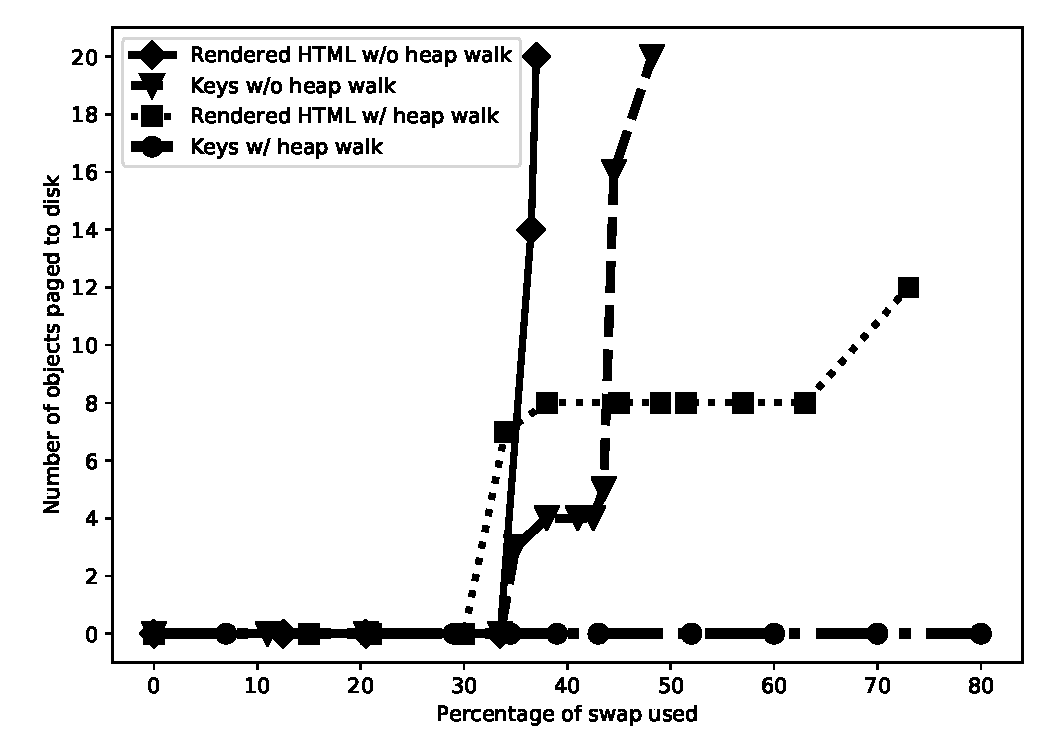
\includegraphics[width=\textwidth]{veil-figs/heapwalk_graph.pdf}
	\caption{The effectiveness of heap walking to prevent secrets from paging out.}
	\label{fig:heapWalking}
\end{figure}

\noindent
{\bf Protecting RAM artifacts:} To determine
whether heap walking can prevent secrets from
paging out, we wrote a C program which gradually
increases its memory pressure. The program allocates
memory without deallocating any, and periodically,
it reads the first byte in every allocated page
to ensure that the OS considers the page to be hot.
We ran the program inside of a QEMU VM with 1 GB
of swap space and 1 GB of RAM. We also ran a browser
inside of the VM. The browser had 20 open tabs.
Each tab had a Uint8Array representing a tab-specific
AES key, and a tab-specific set of strings in its
HTML. The control experiments did not do heap walking.
The test experiments used Veil's heap walking code
to touch the AES key and the renderer state.

The VM used the \texttt{pwritev} system call to
write memory pages to the swap file. To determine
whether secrets paged out as memory pressure
increased, we used strace to log the \texttt{pwritev}
calls. Since each tab contained a set of 
unique byte patterns, we could grep through our
\texttt{pwritev} logs to determine whether secret
RAM artifacts hit the swap file. We ran experiments
for increasing levels of memory pressure until the
VM became unresponsive, at roughly 75\% in-use
swap space.

Figure~\ref{fig:heapWalking} shows the results.
The x-axis varies the memory pressure, and the
y-axis depicts the number of tabs which suffered
data leakage, as determined by greps through the
\texttt{pwritev} log. Heap walking successfully
kept all of the secret keys from paging out, up
to the maximum 75\% of in-use swap space. Without
heap walking, keys begin to page out at 35\%
swap utilization; by 50\%, all keys had swapped
out. Note that the data points do not perfectly
align on the x-axis due to nondeterminism in
when the VM decides to swap data out.

Heap walking was less effective for renderer
memory pages. Those pages swapped out earlier
and immediately in the control case, around
35\% swap utilization. With Veil, renderer state
also began to leak at 35\% utilization, but
Veil still managed to safeguard 12 out of 20 tabs
up to 63\% swap utilization.

% Taking a memory snapshot using VMWare Workstation:
%  \begin{smitemize}
%    \item Load the VM, run a browser, interact with it,
%          then suspend it.
%    \item Use the \texttt{vmss2core} tool to create a
%          core dump. For example: \begin{verbatim}"C:\Program Files (x86)\VMware\VMware Player"\vmss2core Lubuntu-e49257cd.vmss Lubuntu-e49257cd.vmem\end{verbatim}
%    \item The core will be in a file named \texttt{vmss.core0}.
%  \end{smitemize}

% Generating a core dump for a Linux process:
%  \begin{smitemize}
%    \item Get the pid of the process.
%    \item sudo gcore -o XXX.core pid
%    \item strings -e l -a -t x XXX.core | grep YYY
%  \end{smitemize}

\subsubsection{DOM Hiding}
\label{sec:dhEval}

When Veil runs in DOM hiding mode, the client-side page
contains no site-specific, greppable content. Thus,
Veil does not need to perform heap walking (although
Veil does use blinding servers to eliminate information
leakage through name-based system interfaces). We loaded
our test pages in DOM hiding mode, and confirmed the absence
of site-specific content by grepping through VM images as
we did in Section~\ref{sec:privLeaks}. 

\begin{figure}
	\centering
	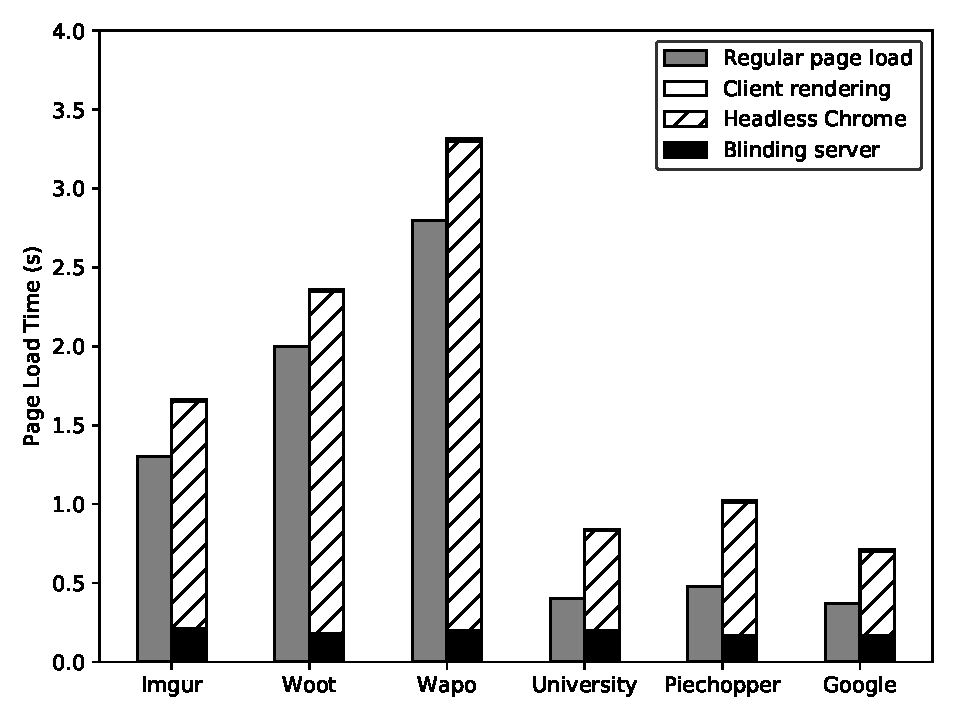
\includegraphics[width=\textwidth]{veil-figs/domhiding_loadtime.pdf}
	\caption{DOM hiding's impact on page load times.}
	\label{fig:dhPageLoad}
\end{figure}

\begin{figure}
	\centering
	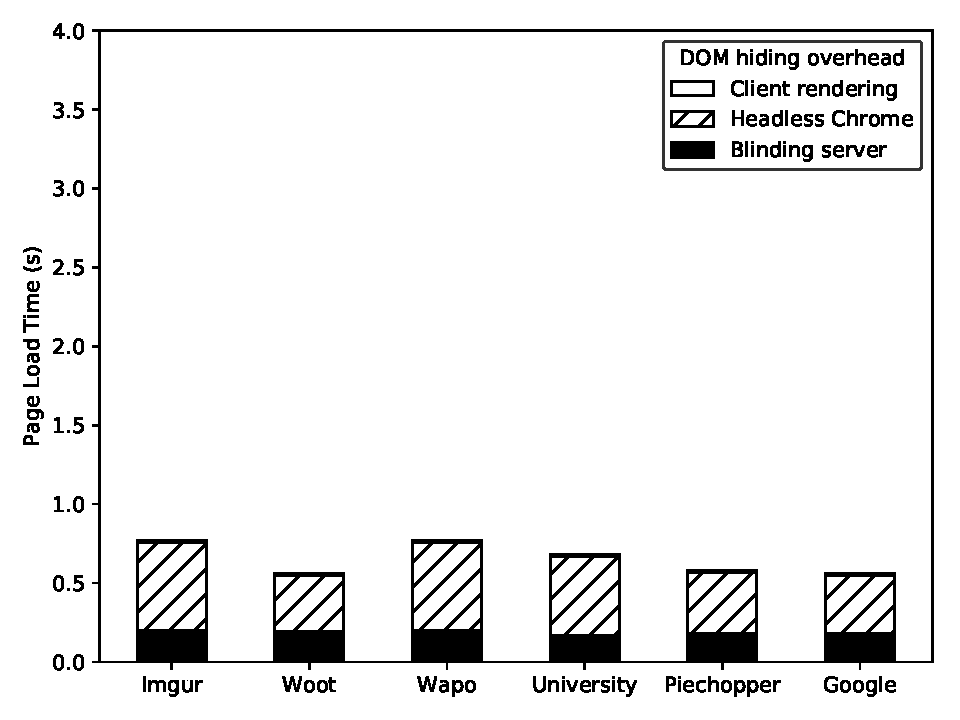
\includegraphics[width=\textwidth]{veil-figs/domhiding_click.pdf}
	\caption{The time that a DOM-hiding page needs to respond to a
		mouse click event.}
	\label{fig:dhClick}
\end{figure}

Figure~\ref{fig:dhPageLoad} evaluates the impact of DOM
hiding on a page's initial load. The client, the blinding
server, and the content server ran on the same machine, to
focus on computational overheads. Figure~\ref{fig:dhPageLoad}
demonstrates that DOM hiding imposed moderate overheads,
with page load times increasing by 1.2x--2.1x.
When Veil runs in DOM hiding mode, image mutation
has to be performed synchronously, for each screenshot
that is returned to a client; screenshotting requires
150ms--180ms, whereas image mutation requires
170ms--200ms.

Figure~\ref{fig:dhClick} shows the time that a DOM-hiding
page needed to respond to a mouse click. Responding to
such a GUI event required the browser to forward the
event to the content provider, and then receive and
display the new screenshot. Once again, the bulk of the
end-to-end time was consumed by the screenshot capture
and the image mutation at the content provider. 

Privacy-sensitive users and web sites are often willing
to trade some performance for better security. For
example, fetching an HTTP object through Tor results in
HTTP-level RTTs of more than a second~\cite{torStats}.
Thus, we believe that the performance of Veil's 
DOM hiding mode is adequate for many sites. However,
Veil's performance may be too slow for sites that
are highly interactive, or require content servers to
frequently and proactively push new images (e.g.,
due to animations in a page). Our next version of
the Veil GUI proxy will grab screenshots directly
from the content server's framebuffer~\cite{framebuffer}
instead of via the comparatively-slow rendering API
that browsers expose~\cite{cvt}; this implementation
change will greatly reduce screenshotting overhead.

\subsubsection{Network Latency}
\label{sec:lat}

\begin{figure}
	\centering
	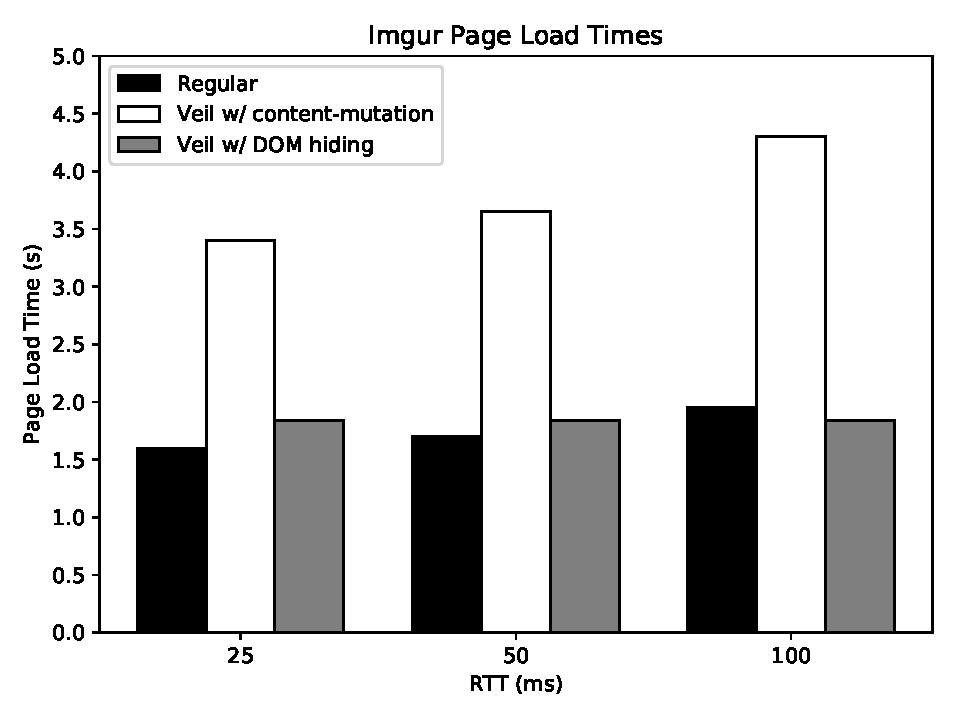
\includegraphics[width=\textwidth]{veil-figs/network_em.pdf}
	\caption[The impact of emulated network latency on page load
	times.]{The impact of emulated network latency on page load
		times. In all cases, the download bandwidth cap
		was 30 Mbps, and the upload bandwidth cap was 10
		Mbps, emulating a broadband connection. Bandwidth
		was not varied because page load times are largely
		governed by network latency, not bandwidth~\cite{gentleaggression}.}
	\label{fig:net_em}
\end{figure}

Figure~\ref{fig:net_em} uses Chrome's built-in network
emulation framework~\cite{chromeThrottle} to compare load times
for three versions of the Imgur page: a normal version;
a Veil version which used content mutation, heap
walking, and encrypted storage; and a Veil version
which used DOM hiding. The DOM hiding variant was largely
insensitive to increased network latency, since loading
a page only required two HTTP-level round trips (one to
fetch the bootstrap page, and another to fetch the initial
screenshot). The other variant of Veil was more sensitive
to network latency. The reason is that, in this version of
the page, the bootstrap code had to fetch multiple objects,
all of which were served from the same blinding server origin
(\texttt{https://veil.io}). Browsers cap the number
of simultaneous connections that a client can make to
a single origin, so the Veil page could not leverage
domain sharding~\cite{domainSharding} to circumvent the
cap. This limitation is not fundamental to Veil's design,
since content providers can shard across multiple blinding
server domains (e.g., \texttt{https://a.veil.io}
and \texttt{https://b.veil.io}). However (and
importantly), if a content provider wishes to use
sharding, the provider must be careful to avoid bias
in the mapping of objects to domains---otherwise,
per-site fingerprints may arise in a page's access
patterns to various domains. Thus, for some content
providers, domain sharding may not be worth the potential
loss in security.

Domain sharding is also relevant to Content Security
Policies (CSPs)~\cite{csp}. A CSP allows a page to restrict the
origins which can provide specific types of content.
For example, a CSP might state that a page can only
load JavaScript from \texttt{https://a.com}, and CSS
from \texttt{https://b.com}. A CSP is expressed as a
server-provided HTTP response header; the CSP is enforced
by the browser. CSPs are useful for preventing cross-site
scripting attacks, but require a page to be able to
explicitly shard content across domains. As discussed
in the last paragraph, Veil can enable sharding at
the cost of reduced security.

\subsection{Related Work}
\label{sec:related}

%{\bf Interactions with the Cloud}\\
%Mylar~\cite{mylar} is a platform for building
%secure web applications atop untrusted servers.
%Mylar only stores encrypted user data on servers,
%and decrypts that data using client-side JavaScript.
%Mylar defines primitives for searching over
%encrypted data and validating the JavaScript code
%that a potentially malicious server returns
%to the browser. Veil focuses on client-side
%privacy issues, but a Veil application could
%be layered atop Mylar to provide server-side
%protections as well.

%\
%{\bf Systems Support for Data Privacy:}
To minimize information leakage via RAM artifacts,
applications can use best practices like pinning
sensitive memory pages, and avoiding excessive
copying of secret data~\cite{harrison07}.
Operating systems and language runtimes can also
scrub deallocated memory as quickly as
possible~\cite{chow05}. Web browsers do not expose
low-level OS interfaces to JavaScript code, so
privacy-preserving sites cannot directly access
raw memory for the purposes of secure deallocation
or pinning. Determining the best way to expose
raw memory to JavaScript is an open research problem,
given the baroque nature of the same-origin policy,
and the fact that the browser itself may contend
with JavaScript code for exclusive access to a
memory page (e.g., to implement garbage collection
or tab discarding~\cite{tabDiscarding}).

An OS can protect RAM artifacts by encrypting
the swap space or the entire file system~\cite{blaze93,provos00,cryptfs}.
Veil's content mutation and DOM hiding allow Veil
to protect RAM artifacts even when a browser does not
run atop an encrypted storage layer. Content mutation
obviously does not provide a cryptographically strong
defense, but DOM hiding allows a Veil site to avoid
sending any site-specific, greppable content to a
client browser.

CleanOS~\cite{cleanOS} is a smartphone OS that
protects sensitive data when mobile devices
are lost or stolen. CleanOS defines sensitive
data objects (SDOs) as Java objects
and files that contain private user data.
CleanOS observes which SDOs are not actively
being used by an application, and encrypts
them; the key is then sent to the cloud, deleted
from the smartphone, and only retrieved when
the SDOs become active again. SDOs could
potentially be used as a building block for
private browsing. However, SDOs are insufficient
for implementing blinded references unless
the SDO abstraction is spread beyond the managed
runtime to the entire OS.

Lacuna~\cite{lacuna} implements private sessions
by running applications inside of VMs. Those VMs
execute atop the Lacuna hypervisor and a modified
Linux host kernel. The hypervisor and the host
kernel collectively implement ``ephemeral'' IO
channels. These encrypted channels allow VMs to
communicate with hardware or small pieces of
trusted code, but only the endpoints can access
raw data---user-mode host processes and the majority
of the host kernel can only see encrypted data.
Lacuna also encrypts swap memory. Upon VM
termination, Lacuna zeros the VM's RAM space and
discards the ephemeral session keys.
PrivExec~\cite{privExec} is similar to Lacuna,
but is implemented as an OS service instead of
a hypervisor.
%
% PrivExec~\cite{privExec} is an OS service that supplies
% privacy-seeking applications with automatically encrypted
% channels to persistent storage. Similar to Lacuna, PrivExec
% associates private processes with ephemeral keys that are
% used to transparently encrypt writes to the file system
% and page file. PrivExec also monitors IPCs to ensure that
% private session data is not leaked to non-private processes.
% Like Lacuna, PrivExec destroys ephemeral keys when applications
% terminate.
%
Lacuna and PrivExec provide stronger forensic
deniability than Veil. However, these systems
force layperson end-users to install and configure
a special runtime; furthermore, private applications
cannot persist data across sessions because keys are
ephemeral.

UCognito~\cite{ucognito} exposes a sandboxed file system
to a private browsing session. The sandboxed file system
resides atop the normal one, absorbing writes made during
private browsing. When the browsing session terminates,
UCognito discards the writes. Like PrivExec and Lacuna,
UCognito requires a modified client-side software stack.
UCognito also does not protect against information leakage
via the non-sandboxed parts of the host OS. For example,
unmodified RAM artifacts may page to the native swap file;
DNS requests are exposed to the host's name resolution
subsystem.

Amazon Silk~\cite{amazon-silk} is a browser used on Amazon
Kindles and uses a technique called remote dependency 
resolution (also known as split browsing)~\cite{rc2, parcel}. 
When the Silk client issues an HTTP request for a web page,
the request actually goes to an Amazon-maintained 
proxy that runs in the cloud. The proxy then uses a headless
browser to load the requested page. Since the proxy lives
in the core of the Internet, the proxy can fetch objects
over low-latency network paths. As the proxy fetches these
objects, they are streamed back to the user. This technique
allows Silk to avoid high last-mile latencies afflicting the path
between the client and Internet core. However, the client-side Silk browser
still loads regular DOM objects, like HTML, Javascript, CSS, etc.,
thus not implementing DOM hiding that exists in Veil. It also
does not protect RAM artifacts or provide content mutation.

Collaborative browsing frameworks~\cite{lowet09,jigsawCollab}
allow multiple users with different browsers to
simultaneously interact with a shared view of a web
page. Like these frameworks, Veil's DOM hiding mode
has to synchronize the GUI inputs and rendering activity
that belong to a canonical version of a page. However,
Veil only needs to support one remote viewer. More
importantly, Veil's DOM hiding mode only exposes the
client browser to generic JavaScript event handlers, as
well as a bitmap display; in contrast, prior collaborative
browsing frameworks replicate a site-specific, canonical
DOM tree on each client browser. Prior frameworks also
do not use blinding servers to hide information from
client-side, name-centric interfaces like the DNS
cache.

Silo~\cite{silo} and the framework of Jiang et
al~\cite{jiang14} use client-side bootstrap
pages which dynamically overwrite themselves
with new content. Silo uses this technique to
layer a delta-encoding protocol atop HTTP;
Jiang's system uses dynamic assembly as a crude
copy-protection mechanism, so that users who
right click and ``Save as'' a page will only
store the initial bootstrap HTML and not the
dynamically assembled content. By itself,
dynamic assembly cannot provide strong privacy
guarantees. For example, blinded URLs are needed
to prevent information leakage through the DNS
cache and the browser cache.

\subsection{Conclusions}
Veil is the first web framework that allows
developers to implement private-session semantics
for their pages. Using the Veil compiler,
developers rewrite pages so that all page content
is hosted by blinding servers. The blinding servers
provide name indirection, preventing sensitive
information from leaking to client-side, name-based
system interfaces. The blinding servers mutate
content, making object fingerprinting more
difficult; rewritten pages also automatically
encrypt client-side persistent storage, and
actively walk the heap to reduce the likelihood
that in-memory RAM artifacts will swap to disk in
cleartext form. In the extreme, Veil transforms
a page into a thin client which does not include
any page-specific, greppable RAM artifacts. Veil
automates much of the effort that is needed to
port a page to Veil, making it easier for
web developers to improve the privacy protections of
their applications.
\section{Splinter: Practical, Private Web Application Queries}
\label{chap:splinter}

\subsection{Motivation}

Web applications are collecting increasing amounts
of data, and this data contains information useful
to both users and businesses. For example,
users can access crowdsourced information,
such as the most up-to-date
traffic data to determine the fastest route.
Similarly, businesses can use this data to better
understand user behavior and better market products. 
Many of these applications currently allow users
to query these datasets, but an increasing number
are allowing businesses and researchers to query
this data. However, the problem is that 
these queries can reveal sensitive information,
such as user behavior, identifiable personal information, 
and business strategy~\cite{narayanan2010myths, narayanan2008robust}.

%Many online services let users query large datasets:
%some examples include restaurant sites, stock quotes,
%medical information, and patents. In these services, 
%any user can query the data, and the datasets themselves
%do not contain sensitive user data. 
%However, web services can infer a great deal of identifiable and sensitive
%user information from these queries, such as her 
%political affiliation, sexual orientation, income,
%medical conditions, behavior, etc.~\cite{narayanan2010myths, narayanan2008robust}.
%Web services can use this information maliciously and put users at risk to practices such as
%discriminatory pricing~\cite{amazon-disc-pricing, price-disc2, hannak2014measuring}.
%For example, online stores have charged users different prices based on location~\cite{price-disc}, and
%travel sites have also increased prices for certain frequently searched flights~\cite{travel-pricing}.
%Even when the services are honest, server compromise and subpoenas can leak the sensitive user
%information collected by these services~\cite{ravichandran2009capturing, yelp-compromise, twitter-compromise}.

This dissertation presents Splinter, a practical system that allows servers
to properly respond to user queries without learning the sensitive information 
present in the queries.
In Splinter, the user divides each query into shares and sends them to different
\emph{providers}, which are services hosting a copy of the dataset (Figure~\ref{fig:overview}).
As long as any one of the providers is honest and does not
collude with the others, the providers cannot discover sensitive
information in the query.
However, given responses from all the providers, the user
can compute the answer to her query.

\begin{figure}
	\centering
	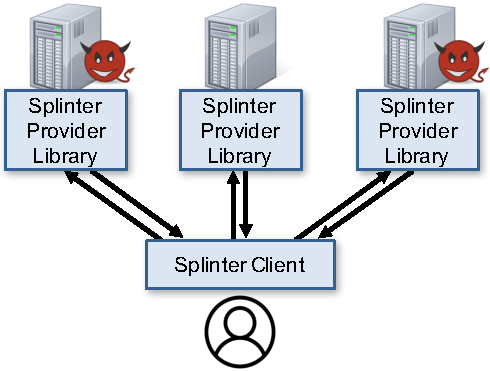
\includegraphics[width=\textwidth]{splinter-figs/overview.pdf}
	\caption[Overview of Splinter architecture.]{
		Splinter architecture. 
		The Splinter client splits each user query into shares and sends them to multiple
		providers. It then combines their results to obtain
		the final answer.
		The user's query remains private as long as any one provider is honest.
	}
	\label{fig:overview}
\end{figure}

Previous private query systems have generally not achieved practical performance
because they use expensive cryptographic primitives and protocols.
For example, systems based on other cryptographic techniques such
as Private Information Retrieval (PIR)~\cite{goldberg,chor1997private,pir-search} 
require many round trips and high bandwidth for complex queries, while systems based on garbled
circuits~\cite{wu2016,lan2016embark,ben2008fairplaymp} have a high computational cost.
These approaches are especially costly for mobile clients on high-latency networks.

Instead, Splinter is the first system to use and extend a recent cryptographic primitive called
Function Secret Sharing (FSS)~\cite{fss, gilboa2014distributed} for private queries.
FSS allows the client to split certain functions into shares that keep parameters of the
function hidden unless all the providers collude.
With judicious use of FSS, many queries can be answered in only a single network round trip
with low CPU and bandwidth costs.

Splinter makes two contributions over previous work on FSS.
First, prior work has only demonstrated efficient FSS protocols for point and interval functions with additive aggregates such as SUMs~\cite{fss}.
We present protocols that support a more complex set of non-additive aggregates such as MAX/MIN and TOPK at low computational and communication cost.
Together, these protocols let Splinter support a subset of SQL that can capture many popular online applications.

Second, we develop an optimized implementation of FSS for modern hardware that leverages AES-NI~\cite{aes-ni} instructions and multicore CPUs.
For example, using the one-way compression functions that utilize modern AES instruction sets, our implementation is 2.5$\times$ faster per core than a na\"ive implementation of FSS.
Together, these optimizations let Splinter query datasets with millions of records at sub-second latency on a single server.

We evaluate Splinter by implementing 
three applications over it: a restaurant review site similar to Yelp, 
airline ticket search, and map routing.
For all of our applications, Splinter can execute queries in less than 1.6 seconds, at a cost of less than 0.05 cents in server resources on Amazon EC2.
%Splinter's low cost means that providers could profitably run a Splinter-based service
%similar to OpenStreetMap routing~\cite{osm}, an open-source maps service, while only charging users a few dollars per month.

%Finally, Splinter does have some limitations.
%First, FSS, like PIR, requires scanning the whole input dataset on
%every query, to prevent providers from figuring out which records have
%been accessed.
%Second, Splinter does not support some SQL features, such as private join conditions.
%Despite these limitations, we show that Splinter is practical on large
%real-world datasets, such as maps, and can support many of today's online applications.
%Because human-created datasets are unlikely to grow faster than
%hardware capabilities in the future, we believe Splinter's techniques will only
%become more practical over time.

%FSS improves over PIR 
%because it allows matching \textit{multiple} records efficiently in one scan
%while practical PIR schemes can only match a single record in one scan. 
%Therefore, to the best of our knowledge,
%Splinter is the first system to practically preserve the privacy 
%of queries on large public datasets.

%In summary, our contributions are:
%\begin{itemize}
%	\item{Splinter, a private query system that achieves significantly lower CPU and communication costs than previous systems.}
%	\item{New protocols that extend FSS to complex queries with non-additive aggregates, e.g., TOPK and MAX.}
%	\item{An optimized FSS implementation for modern CPUs.}
%	\item{An evaluation of Splinter on realistic applications.}
%\end{itemize}

\subsection{Splinter Architecture}
\label{sec:goals}

Splinter aims to protect sensitive information in users' queries
from providers. This section provides an overview of Splinter's architecture,
security goals, and threat model.

\subsubsection{Splinter Overview}
\label{sec:model}
There are two main principals in Splinter: the \emph{user} and the \emph{providers}.
Each provider hosts a copy of the data. Providers can 
retrieve this data from a public repository or mirror site.
Similarly, data owners, like Yelp and Google Maps, can license
data to be hosted on these providers. In both scenarios,
the providers store the data in cleartext. 

Users issue queries to the provider.
For a given user query, all the providers have to run it on the same
view of the data. Maintaining data consistency
from mirror sites is beyond the scope of this dissertation, but
standard techniques can be used~\cite{tewari2002wcdp,chi2008novel}.
%For example, OpenStreetMap~\cite{osm} publishes publicly available 
%map, point-of-interest, and traffic data. 

As shown in Figure~\ref{fig:overview}, 
to issue a query in Splinter, a user
splits her query into \textit{shares}, using the Splinter client,
and submits each share to a different provider.
The user can select any providers of her choice that host the dataset.
The providers use their shares to execute the user's query 
over the cleartext data, using the Splinter provider library. 
As long as one provider is \textit{honest}
(does not collude with others), the user's sensitive information in the original query
remains private. When the user receives the corresponding responses from the providers,
she combines them to obtain the final answer to her original query. 
%In Section~\ref{sec:queries},
%we will describe in more detail how the user creates these function shares and how
%the provider uses them to execute the user's query.

\subsubsection{Use Cases}
\label{sec:splinter_cases}
Although Splinter can handle complex queries, it is not
meant as a private query system for all SQL-like databases.
Splinter's use cases are similar to those of PIR. More specifically,
the queries contain sensitive user information and need to be 
protected, but the database itself does not contain
sensitive user information. For example, users might not
want to reveal where they are traveling to Google when searching
for directions. Similarly, data analysts might want to hide
their query parameters because they might leak trade
secrets for their algorithms.

Splinter works well for applications with large databases
and regular updates because downloading the whole
database and receiving updates would be more expensive in terms
of bandwidth than querying the Splinter service. Services,
like flight prices, map navigation, stock prices, 
and domain name availability searches, are good fits for Splinter.
In Section~\ref{sec:communication}, we discuss and 
quantify the "break even" point for our case studies.

Even if it is more efficient for the user to download the whole
database and updates, Splinter can still be useful.
Many applications might enforce rate limiting or query restrictions
to prevent users from accessing the whole database
because the data might contain proprietary information.
For example, Yelp might allow limited querying
for data scientists through an API but not give complete access to their dataset. 

\subsubsection{Security Goals}
\label{sec:query_model}
The goal of Splinter is to hide sensitive parameters in
a user's query.
Specifically, Splinter lets users run \emph{parametrized queries}, 
where both the parameters and query results are hidden from providers.
For example, consider the following query, which finds the 10 cheapest flights between a source and destination:
\begin{verbatim}
SELECT TOP 10 flightid FROM flights
WHERE source = ? AND dest = ? 
ORDER BY price
\end{verbatim}
Splinter hides the information represented by the questions marks, i.e.,
the source and destination in this example.
The column names being selected and filtered are not hidden.
Finally, Splinter also hides the query's results---otherwise,
these might be used to infer the source and destination. 
Splinter supports a subset of the SQL language, which we describe in Section~\ref{sec:querymodel}.
Note that the data is in cleartext, and Splinter's goal is not to protect the data on 
the server side. However, the data owners or providers might have 
mechanisms in place to limit user access to this data.

The easiest way to achieve this property would be for users to download the whole database
and run the queries locally. However, as described in Section~\ref{sec:splinter_cases}
downloading so much data might not be feasible. 
%However, this requires substantial bandwidth and computation for the user.
%Moreover, many datasets change constantly, e.g., to include traffic information or new product reviews.
%It would be impractical for the user to continuously download these updates.
%Therefore, our performance objective is to minimize computation and communication costs.
%For a database of $n$ records, Splinter only requires $O(n \log n)$ computation at the
%providers and $O(\log n)$ communication (Section~\ref{sec:complex}).

\subsubsection{Threat Model}
Splinter keeps the parameters in the user's query hidden
as long as at least one of the user-chosen providers does not collude with others. 
Splinter also assumes these providers are \textit{honest but curious}: a provider can observe the interactions between
itself and the client, but 
Splinter does not protect against providers returning incorrect results or maliciously modifying the dataset.

We assume the data is in cleartext and that the user communicates with each provider through a secure channel (e.g., using SSL),
and that the user's Splinter client is uncompromised. 
%Protecting attacks on a user's machine are outside of the scope of Splinter.
Our cryptographic assumptions are standard.
We only assume the existence of one-way functions.
%In our implementation for multiple providers, the security of Paillier encryption~\cite{paillier} is also assumed.


\subsection{Function Secret Sharing}
\label{sec:queries}
In this section, we give an overview of Function Secret Sharing (FSS),
the main primitive used in Splinter, and show how to use it in simple queries.
Sections~\ref{sec:querymodel} and~\ref{sec:complex} then describe Splinter's full
query model and our new techniques for more complex queries.

\subsubsection{Overview of Function Secret Sharing}
\label{sec:fss_overview}
Function Secret Sharing~\cite{fss} lets a client divide
a function $f$ into \textit{function shares} 
$f_1,f_2,\dots,f_k$ so that multiple parties
can help evaluate $f$ without learning certain of its parameters.
These shares have the following properties:

\begin{itemize}
	\item{They are close in size to a description of $f$.}
	\item{They can be evaluated quickly (similar in time to $f$).}
	\item{They sum to the original function $f$.
		That is, for any input $x$, $\sum\limits_{i=1}^k f_i(x) = f(x)$. We 
		assume that all computations are done over $\mathbb{Z}_{2^m}$, 
		where $m$ is the number of bits in the output range. }
	\item{Given any $k-1$ shares $f_i$, an adversary cannot recover the parameters 
		of $f$.}
\end{itemize} 

Although it is possible to perform
FSS for arbitrary functions~\cite{dodis2016spooky}, 
practical FSS protocols only exist for \emph{point} and \emph{interval} functions.
These take the following forms:
\begin{itemize}
	\item Point functions $f_a$ are defined as $f_a(x)=1$ if $x=a$ or 0 otherwise.
	\item Interval functions are defined as $f_{a,b}(x)=1$ if $a \le x \le b$ or 0 otherwise.
\end{itemize}

In both cases, FSS keeps the parameters $a$ and $b$ private: an adversary can tell that
it was given a share of a point or interval function, but cannot find $a$ and $b$.
In Splinter, we use the FSS scheme of Boyle et al.~\cite{fss}.
Under this scheme, the shares $f_i$ for both functions require $O(\lambda n)$ bits to
describe and $O(\lambda n)$ bit operations to evaluate for a security parameter $\lambda$ (the size
of cryptographic keys), and $n$ is the number of bits in the input domain.
%This contrasts to $O(n)$ bits and operations to describe and evaluate the original
%functions.

\subsubsection{Using FSS for Database Queries}
\label{sec:fss_queries}

We can use the additive nature of FSS shares to run private queries over
an entire table in addition to a single data record.
We illustrate here with two examples.

\begin{figure}
	\centering
	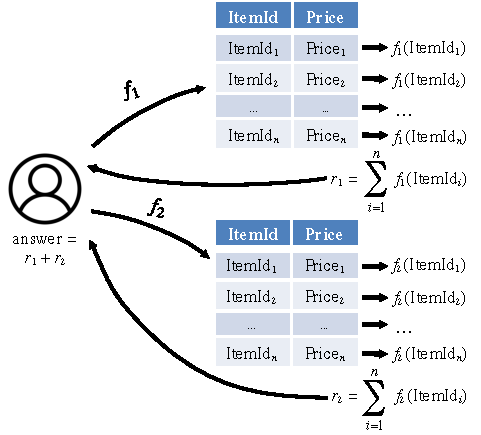
\includegraphics[width=\textwidth]{splinter-figs/fss.pdf}
	\caption{Overview of how FSS can be applied to database records
		on two providers to perform a COUNT query.}
	\label{fig:fss_overview}
\end{figure}


\paragraph{Example: COUNT query.}
Suppose that the user wants to run the following query on
a table served by Splinter:
\begin{verbatim}
SELECT COUNT(*) FROM items WHERE ItemId = ?
\end{verbatim}

Here, `\texttt{?}' denotes a parameter that the user would like to keep
private; for example, suppose the user is searching for \texttt{ItemId = 5},
but does not want to reveal this value.

To run this query, the Splinter client defines a point function $f(x)=1$ if $x=5$
or 0 otherwise.
It then divides this function into function shares $f_1,\dots,f_n$ and
distributes them to the providers, as shown in Figure~\ref{fig:fss_overview}.
For simplicity, suppose that there are two providers, who receive shares
$f_1$ and $f_2$.
Because these shares are additive, we know that $f_1(x)+f_2(x)=f(x)$
for every input $x$.
Thus, each provider $p$ can compute $f_p(\mathrm{ItemId})$ for every ItemId in the
database table, and send back $r_p = \sum_{i=1}^n f_p(\mathrm{ItemId}_i)$
to the client.
The client then computes $r_1 + r_2$, which is equal
to $\sum_{i=1}^n f(\mathrm{ItemId}_i)$, that is, the count of all matching
records in the table.

\begin{figure}
	\centering
		\begin{tabular}{cccc}
			\toprule
			\bf ItemId & \bf Price & $f_1$(ItemId) & $f_2$(ItemId) \\
			\midrule
			5 & 8 & 10 & -9 \\
			1 & 8 & 3 & -3 \\
			5 & 9 & 10 & -9 \\
			\bottomrule
		\end{tabular}
	\caption[Function Secret Sharing example outputs.]{Simple example table with outputs for the FSS function shares $f_1$, $f_2$ applied to the ItemId column. 
		The function
		is a point function that returns 1 if the input is 5, and 0 otherwise.
		All outputs are integers modulo $2^m$ for some $m$.
	}
	\label{fig:fssExample2}
\end{figure}

To make this more concrete, Figure~\ref{fig:fssExample2} shows an example
table and some sample outputs of the function shares, $f_1$ and $f_2$,
applied to the ItemId column. 
There are a few important observations. First, to each provider,
the outputs of their function share seem random. Consequently, the provider does not learn
the original function $f$ and the parameter ``5''. Second, 
because $f$ evaluates 
to 1 on inputs of 5, $f_1(\mathrm{ItemId}) + f_2(\mathrm{ItemId}) = 1$ for rows 1 and 3. 
Similarly, $f_1(\mathrm{ItemId}) + f_2(\mathrm{ItemId})=0$ for row 2.
Therefore, when summed across the providers, each row
contributes 1 (if it matches) or 0 (if it does not match) to the 
final result. 
Finally, each provider aggregates the outputs of their shares by summing them. 
In the example, one provider returns 23 to the client, and
the other returns -21.
The sum of these is the correct query output, 2.

This additivity of FSS enables Splinter
to have \textit{low communication costs} for aggregate queries, by aggregating
data locally on each provider.
%Adding values locally in the provider 
%does not leak any information because each value appears random to the provider.

\paragraph{Example: SUM query.}
Suppose that instead of a COUNT, we wanted to run the following SUM query:
\begin{verbatim}
SELECT SUM(Price) FROM items WHERE ItemId=?
\end{verbatim}

This query can be executed privately with a small extension to the COUNT scheme.
As in COUNT, we define a point function $f$ for our secret predicate, e.g.,
$f(x)=1$ if $x=5$ and 0 otherwise.
We divide this function into shares $f_1$ and $f_2$.
However, instead of computing
$r_p = \sum_{i=1}^n f_p(\mathrm{ItemId}_i)$,
each provider $p$ computes
$$r_p = \sum_{i=1}^n f_p(\mathrm{ItemId}_i) \cdot \mathrm{Price}_i$$

As before, $r_1 + r_2$ is the correct answer of the query,
that is, $\sum_{i=1}^n f(\mathrm{ItemId}_i) \cdot \mathrm{Price}_i$.
We add in each row's price, $\mathrm{Price}_i$, 0 times if the ItemId is equal to 5,
and 1 time if it does not equal 5.

\subsection{Splinter Query Model}
\label{sec:querymodel}

Beyond the simple SUM and COUNT queries in the previous section, 
we have developed
protocols to execute a large class of queries using FSS, including
non-additive aggregates such as MAX and MIN, and queries that return multiple
individual records instead of an aggregate.
For all these queries, our protocols are efficient in both
computation and communication.
On a database of $n$ records, all queries can be executed in $O(n \log n)$ time
and $O(\log n)$ communication rounds, and most only require 1 or 2 communication rounds
(Figure~\ref{fig:complexity} on page~\pageref{fig:complexity}).

\begin{figure}
	%\small
	\centering
	\fbox{
		\begin{minipage}{0.7\textwidth}
			\begin{description}
				\item[\normalfont Query format:] \hspace{1mm} \\
				SELECT \emph{aggregate}$_1$, \emph{aggregate}$_2$, $\dots$ \\
				FROM \emph{table}\\
				WHERE \emph{condition}\\
				$[$GROUP BY \emph{expr}$_1$, \emph{expr}$_2$, $\dots]$
				
				\item[\normalfont \it aggregate:] \mbox{}\\[-1.5\baselineskip]
				\begin{itemize}
					\item COUNT | SUM | AVG | STDEV (\emph{expr})
					\item MAX | MIN (\emph{expr})
					\item TOPK (\emph{expr}, $k$, \emph{sort\_expr})
					\item HISTOGRAM (\emph{expr}, \emph{bins})
				\end{itemize}
				
				\item[\normalfont \it condition:] \mbox{}\\[-1.5\baselineskip]
				\begin{itemize}
					\item \emph{expr} = \emph{secret}
					\item \emph{secret}$_1$ $\le$ \emph{expr} $\le$ \emph{secret}$_2$
					\item AND of `=' conditions and up to one interval
					\item OR of multiple disjoint conditions\\
					(e.g., \texttt{country="UK" OR country="USA"})
				\end{itemize}
				
				\item[\normalfont \it expr:] any public function of the fields in a table
				row\\(e.g., \texttt{ItemId + 1} or \texttt{Price * Tax})
				
			\end{description}
		\end{minipage}
	}
	
	\caption[Splinter query format.]{Splinter query format.
		The TOPK aggregate returns the top $k$ values of \emph{expr} for matching rows
		in the query, sorting them by \emph{sort\_expr}.
		In conditions, the parameters labeled \emph{secret} are hidden from the
		providers.
	}
	\label{fig:suppq}
\end{figure}

Figure~\ref{fig:suppq} describes Splinter's supported queries using SQL syntax.
Most operators are self-explanatory.
The only exception is TOPK, which is used to return up to $k$ individual records
matching a predicate, sorting them by some expression \emph{sort\_expr}.
This operator can be used to implement \texttt{SELECT...LIMIT} queries, but
we show it as a single ``aggregate'' to simplify our exposition.
To keep the number of matching records hidden from providers, the
protocol always pads its result to exactly $k$ records.

%Note also that all queries return a bounded amount of data---there is no way to
%select arbitrarily many rows.
%This is expected given our security model: if we allowed variable-length
%results, the providers might learn something about the query from the number
%of rows sent back.

Although Splinter does not support all of SQL, we found it expressive enough to
support many real-world query services over public data.
We examined various websites, including Yelp, Hotels.com, and Kayak, and found
we can support most of their search features as shown in Section~\ref{sec:case_studies}.

Finally, Splinter only ``natively'' supports fixed-width integer data
types. However, such integers can also be used to encode strings and
fixed-precision floating point numbers (e.g., SQL DECIMALs).
We use them to represent other types of data in our sample applications.

\subsection{Executing Splinter Queries}
\label{sec:complex}

Given a query in Splinter's query format (Figure~\ref{fig:suppq}), the system executes
it using the following steps:

\begin{enumerate}
	\item The Splinter client builds function shares for the condition in the query,
	as we shall describe in Section~\ref{sec:complex-conditions}.
	\item The client sends the query with all the secret parameters removed to
	each provider, along with that provider's share of the condition function.
	\item If the query has a GROUP BY, each provider divides its data into
	groups using the grouping expressions; otherwise, it treats the whole table
	as one group.
	\item \label{agg-step}
	For each group and each aggregate in the query, the provider runs an
	evaluation protocol that depends on the aggregate function and on
	properties of the condition. We describe these protocols in
	Section~\ref{sec:complex-aggregates}.
	Some of the protocols require
	further communication with the client, in which case the provider
	batches its communication for all grouping keys together.
\end{enumerate}

The main challenge in developing Splinter is designing efficient execution protocols
for Splinter's complex conditions and aggregates (Step~\ref{agg-step}).
Our contribution is multiple protocols that can execute non-additive
aggregates with low computation and communication costs.

One key insight that pervades our design is that \emph{the best strategy to
	compute each aggregate depends on properties of the condition function}.
For example, if we know that the condition can only match one value of
the expression it takes as input, we can simply compute the aggregate's result
for \emph{all} distinct values of the expression in the data, and then use a point
function to return just one of these results to the client.
On the other hand, if the condition can match multiple values, we need a
different strategy that can combine results across the matching values.
To reason about these properties, we define three \emph{condition classes}
that we then use in aggregate evaluation.

\subsubsection{Condition Types and Classes}
\label{sec:complex-conditions}

For any condition $c$, the Splinter client defines a function $f_c$
that evaluates to 1 on rows where $c$ is true and 0 otherwise, and divides
$f_c$ into shares for each provider.
Given a condition $c$, let $E_c = (e_1, \dots, e_t)$ be the list of
expressions referenced in $c$ (the \emph{expr} parameters in its clauses).
Because the best strategy for evaluating aggregates depends on $c$, we
divide conditions into three classes:
\begin{itemize}
	\item \emph{Single-value conditions.} These are conditions that can only be
	true on one combination of the values of $(e_1, \dots, e_t)$.
	For example, conditions consisting of an AND of `='
	clauses are single-value.
	\item \emph{Interval conditions.} These are conditions where the input
	expressions $e_1,\dots,e_t$ can be ordered such that $c$ is true on an
	interval of the range of values $e_1||e_2||\dots||e_t$ (where $||$ denotes
	string concatenation).
	\item \emph{Disjoint conditions,} i.e., all other conditions.
\end{itemize}

The condition types described in our query model (Figure~\ref{fig:suppq})
can all be converted into sharable functions, and categorized into these classes,
as follows:

\paragraph{Equality-only conditions.}
Conditions of the form
$\mathit{e}_1=\mathit{secret}_1$ AND $\dots$ AND
$\mathit{e}_t=\mathit{secret}_t$
can be executed as a single point function on the binary string
$\mathit{e}_1||\dots||\mathit{e}_t$.
This is simply a point function that can be shared using existing
FSS schemes~\cite{fss}.
These conditions are also single-value.

\paragraph{Interval and equality.}
Conditions of the form
$\mathit{e}_1=\mathit{secret}_1$ AND $\dots$ AND
$\mathit{e}_{t-1}=\mathit{secret}_{t-1}$ AND
$\mathit{secret}_{t} \le \mathit{e}_{t} \le \mathit{secret}_{t+1}$
can be executed as a single interval function on the binary string
$\mathit{e}_1||\dots||\mathit{e}_t$.
This is again supported by existing FSS schemes~\cite{fss}, and is
an interval condition.

\paragraph{Disjoint OR.}
Suppose that $c_1,\dots,c_t$ are \emph{disjoint} conditions that can be
represented using functions $f_{c_1}, \dots, f_{c_t}$.
Then $c = c_1$ OR$\dots$OR $c_t$ is captured by
$f_c = f_{c_1} + \dots + f_{c_t}$.
We share this function across providers by simply giving them shares of
the underlying functions $f_{c_i}$.
In the general case, however, $c$ is a disjoint condition where we
cannot say much about which inputs give 0 or 1.

%\footnote{
%Note also that adding the $f_i$s does not work for overlapping OR
%clauses. However, disjoint clauses are still
%useful for many real-world queries, e.g., searching for restaurants that are
%either Chinese or Indian.
%\}

\subsubsection{Aggregate Evaluation}
\label{sec:complex-aggregates}

%Our aggregate evaluation protocols depend on both the aggregate function and the
%condition class in the query.

\subsubsubsection{Sum-Based Aggregates}
To evaluate SUM, COUNT, AVG, STDEV and HISTOGRAM, Splinter
sums one or more values for each row regardless of the condition
function class.
For SUM and COUNT, each provider sums the expression being aggregated or a 1 for each
row and multiplies it by $f_i(\mathrm{row})$, its share of the condition
function, as in Section~\ref{sec:fss_queries}.
Computing AVG($x$) for an expression $x$, requires finding SUM($x$) and COUNT($x$),
while computing STDEV($x$) requires finding these values and SUM($x^2$).
Finally, computing a HISTOGRAM into bin boundaries provided by the user simply
requires tracking one count per bin, and adding each row's result to the
count for its bin. Note that the binning expression is not
private---only information about which rows pass the query's condition function.

\subsubsubsection{MAX and MIN}
\label{sec:min-max}
Suppose we are given a query to find MAX($e_0$) WHERE $c(e_1,\dots,e_t)$,
for expressions $e_0,\dots,e_t$.
The best evaluation strategy depends on the class of the condition $c$.

\paragraph{Single-value conditions.} If $c$ is only true for one combination
of the values $e_1,\dots,e_t$, each provider starts by evaluating the query
\begin{Verbatim}[commandchars=\\\{\},codes={\catcode`$=3\catcode`_=8}]
SELECT MAX($e_0$) FROM data GROUP BY $e_1,\dots,e_t$
\end{Verbatim}
This query gives an \emph{intermediate table} with the tuples $(e_1,\dots,e_t)$
as keys and $\mathrm{MAX}(e_0)$ as values.
Next, each provider computes $\sum \mathrm{MAX}(e_0) \cdot f_i(e_1,\dots,e_t)$
across the rows of the intermediate table, where $f_i$ is its share of the
condition function.
This sum will add a 0 for each non-matching row and $\mathrm{MAX}(e_0)$ for the
matching row, thus returning the right value.
Note that if the original table had $n$ rows, the intermediate table can be built
in $O(n)$ time and space using a hash table.

\paragraph{Interval conditions.}
Suppose that $c$ is true if and only if $e_1||\dots||e_t$ is in an interval $[a,b]$,
where $a$ and $b$ are secret parameters.
As in the single-value case, the providers can build a data structure that helps
them evaluate the query without knowing $a$ and $b$.
%The protocol runs as follows:

In this case, each provider builds an array $A$ of entries $(k,v)$, where the keys are all
values of $e_1||\dots||e_t$ in lexicographic order, and the values are $\mathrm{MAX}(e_0)$
for each key.
It then computes $\mathrm{MAX}(A[i..j])$ for all \emph{power-of-2 aligned} intervals
of the array $A$ (Figure~\ref{fig:complex-max-tree}).
This data structure is similar to a Fenwick tree~\cite{fenwick-trees}.

%For example, if $A$ has 6 elements, the provider will compute MAXes on
%$A[0..1]$, $A[2..3]$, $A[4..5]$ and $A[0..3]$.

\begin{figure}
	\centering
	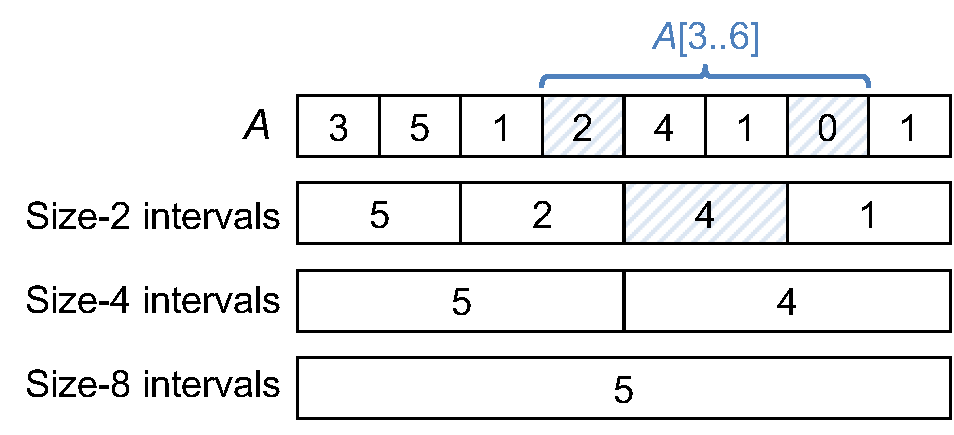
\includegraphics[width=\textwidth]{splinter-figs/complex_max_tree.pdf}
	\caption[Data structure for querying MAX on intervals.]{Data structure for querying MAX on intervals.
		We find the MAX on each power-of-2 aligned interval in the array,
		of which there are $O(n)$ total.
		Then, any interval query requires retrieving $O(\log n)$ of these
		values. For example, to find $MAX(A[3..6])$, we need two
		size-1 intervals and one size-2.
	}
	\label{fig:complex-max-tree}
\end{figure}

Query evaluation then proceeds in two rounds.
First, Splinter counts how many keys in $A$ are less than $a$ and how many are less than
$b$: the client sends the providers shares of the interval functions
$k \in [0,a-1]$ and $k \in [0,b-1]$, and the providers apply these to all keys $k$
and return their results.
This lets the client find indices $i$ and $j$ in $A$
such that all the keys $k \in [a,b]$ are in $A[i..j]$.

Second, the client sends each provider shares of new point functions that select
up to two intervals of size 1, up to two intervals of size 2, etc out of the
power-of-2 sized intervals that the providers computed MAXes on, so as to cover
exactly $A[i..j]$.
Note that any integer interval can be covered using at most 2 intervals of each power of 2.
The providers evaluate these functions to return the MAXes for the selected intervals,
and the client combines these $O(\log n)$ MAXes to find the overall MAX on $A[i..j]$.\footnote{
	To hide which sizes of intervals were actually required, the client should always request 2 intervals
	of each size and ignore unneeded ones.
}

For a table of size $n$, this protocol requires $O(n \log n)$ time at each provider
(to sort the data to build $A$, and then to answer $O(\log n)$ point function queries).
It also only requires two communication rounds, and $O(\log n)$ communication bandwidth.
The same protocol can be used for other associative aggregates, such as products.

\paragraph{Disjoint conditions.}
If we must find MAX($e_0$) WHERE $c(e_1,\dots,e_t)$ but know nothing about $c$,
Splinter builds an array $A$ of all rows in the dataset sorted by $e_0$.
Finding MAX($e_0$) WHERE $c$ is then equivalent to finding the largest index $i$
in $A$ such that $c(A[i])$ is true.
To do this, Splinter uses binary search.
The client repeatedly sends private queries of the form
\begin{Verbatim}[commandchars=\\\{\},codes={\catcode`$=3\catcode`_=8}]
SELECT COUNT(*) FROM $A$
WHERE $c(e_1,\dots,e_t)$ AND $\mathit{index}\in[\mathit{secret}_1,\mathit{secret}_2],$
\end{Verbatim}
where \textit{index} represents the index of each row in $A$ and the interval for it is kept
private. 
%(We shall discuss how to do this.)
By searching for secret intervals in decreasing power-of-2 sizes, the client can find the
largest index $i$ such that $c(A[i])$ is true.
For example, if we had an array $A$ of size 8 with largest matching element at $i=5$,
the client would probe $A[0..3]$, $A[4..7]$, $A[4..5]$, $A[6..7]$ and finally $A[4]$ to
find that 5 is the largest matching index.

Normally, ANDing the new condition $\mathit{index}\in[\mathit{secret}_1,\mathit{secret}_2]$
with $c$ would cause problems, because the resulting conditions might no longer be in
Splinter's supported condition format (ANDs with at most one interval and ORs of
disjoint clauses).
Fortunately, because the intervals in our condition are always power-of-2 aligned,
it can also be written as an equality on the first $k$ bits of \emph{index}.
For example, supposing that \emph{index} is a 3-bit value, the condition
$\mathit{index} \in [4,5]$ can be written as $\mathit{index}_{0,1} =$ ``10'', where
$\mathit{index}_{0,1}$ is the first two bits of \emph{index}.
This lets us AND the condition into all clauses of $c$.

Once the client has found the largest matching index $i$, it runs one
more query with a point function to select the row with $index = i$.
The whole protocol requires $O(\log n)$ communication rounds
and $O(n \log n)$ computation and works well if $c$ has many conditions. 

However, if $c$ has a small number of OR clauses, an optimization is to run
one query for each clause in parallel. The user then resolves
the responses locally to find the answer to the original query.
Although doing this optimization requires more bandwidth because the returned
result size is larger, it avoids the $O(\log n)$ communication rounds and 
the $O(n\log n)$ computation.

\subsubsubsection{TOPK}
\label{sec:topk}
Our protocols for evaluating TOPK are similar to those for MAX and MIN.
Suppose we are given a query to find TOPK($e$, $k$, $e_\mathrm{sort}$) WHERE $c(e_1,\dots,e_t)$.
The evaluation strategy depends on the class of the condition $c$.

\paragraph{Single-value conditions.} If $c$ is only true for one combination
of $e_1,\dots,e_t$, each provider starts by evaluating
\begin{Verbatim}[commandchars=\\\{\},codes={\catcode`$=3\catcode`_=8}]
SELECT TOPK($e,$ $k,$ $e_\mathrm{sort}$) FROM data
GROUP BY $e_1,\dots,e_t$
\end{Verbatim}
This gives an intermediate table with the tuples $(e_1,\dots,e_t)$
as keys and TOPK$(\cdot)$ for each group as values, from which we can select
the single row matching $c$ as in MAX.

\paragraph{Interval conditions.}
Here, the providers build the same auxiliary array $A$ as
in MAX, storing the TOPK for each key instead.
They then compute the TOPKs for power-of-2 aligned intervals in this array.
The client finds the interval $A[i..j]$ it needs to query, extracts the top $k$ values
for power-of-2 intervals covering it, and finds the overall top $k$.
As in MAX, this protocol requires 2 rounds and $O(\log n)$ communication bandwidth.

\paragraph{Disjoint conditions.}
Finding TOPK for disjoint conditions is different from MAX because we need to return
multiple records instead of just the largest record in the table that matches $c$.
This protocol proceeds as follows:
\begin{enumerate}
	\item The providers sort the whole table by $e_\mathrm{sort}$ to create an auxiliary array $A$.
	\item The client uses binary search to find indices $i$ and $j$ in $A$ such that the top $k$
	items matching $c$ are in $A[i..j]$. This is done the same way as in MAX, but searching for
	the largest indices where the count of later items matching $c$ is 0 and $k$.
	\item The client uses a sampling technique (Section~\ref{sec:sampling}) to extract
	the $k$ records from $A[i..j]$ that match $c$. Intuitively, although we do not know which rows
	these are, we build a result table of $>k$ values initialized to 0, and add the FSS share
	for each row of the data to one row in the result
	table, chosen by a hash. This scheme extracts all matching
	records with high probability.
\end{enumerate}
This protocol needs $O(\log n)$ communication rounds
and $O(n \log n)$ computation if there are many clauses, but like the protocol for MAX,
if the number of clauses in $c$ is small,
the user can issue parallel queries for each clause to reduce the communication rounds
and computation.

\subsubsection{Extracting Disjoint Records with FSS}
\label{sec:sampling}

Here, we describe our sampling-based technique for returning multiple records using FSS, used in TOPK queries with disjoint conditions (Section~\ref{sec:topk}).
Given a table $T$ of records and a condition $c$ that matches up to $k$ records, we wish to return those records to the client with high probability without revealing $c$.

To solve this problem, the providers each create a result table $R$ of size $l > k$, containing (value, count) columns all initialized to 0.
They then iterate through the records and choose a result row to update for each record based on a hash function $h$ of its index $i$.
For each record $r$, each provider adds $1 \cdot f_c(r)$ to $R[h(i)]$.count
and $r \cdot f_c(r)$ to $R[h(i)]$.value, where $f_c$ is its share of the condition $c$.
The client then adds up the $R$ tables from all the providers to build up a single table,
which contains a value and count for all indices that a record matching $c$ hashed into.

Given this information, the client can tell how many records hashed into each
index: entries with count=1 have only one record, which can be read from the entry's value.
Unfortunately, entries with higher counts hold multiple records that were added together in
the value field.
To recover these entries, the client can run the same process multiple times in parallel with
different hash functions $h$.

In general, for any given value of $r$ and $k$, the probability of a given record colliding with another under each hash function is a constant (e.g., it is less than $1/3$ for $r=3k$).
Repeating this process with more hash functions causes the probability to fall exponentially.
Thus, for any $k$, we can return all the distinct results with high probability using only $O(\log k)$
hash functions and hence only $O(\log k)$ extra communication bandwidth.

\subsubsection{Complexity}

\begin{figure}
	\centering
		\begin{tabular}{ccccc}
			\toprule
			\bf Aggregate & \bf Condition & \bf Time & \bf Rounds & \bf Bandwidth \\
			\midrule
			Sum-based & any & $O(n)$ & $1$ & $O(1)$ \\
			\midrule
			MAX/MIN & 1-value & $O(n)$ & $1$ & $O(1)$ \\
			MAX/MIN & interval & $O(n \log n)$ & $2$ & $O(\log n)$ \\
			MAX/MIN & disjoint & $O(n \log n)$ & $O(\log n)$ & $O(\log n)$ \\
			\midrule
			TOPK & 1-value & $O(n)$ & $1$ & $O(1)$ \\
			TOPK & interval & $O(n \log n)$ & $2$ & $O(\log n)$ \\
			TOPK & disjoint & $O(n \log n)$ & $O(\log n)$ & $O(\log n)$ \\
			\bottomrule
		\end{tabular}
	\caption[Complexity of Splinter's query evaluation protocols.]{Complexity of Splinter's query evaluation protocols for a database of size $n$.
		For bandwidth, we report the multiplier over the query's normal result size.
	}
	\label{fig:complexity}
\end{figure}

Figure~\ref{fig:complexity} summarizes the complexity of Splinter's query evaluation protocols
based on the aggregates and condition classes used.
We note that in all cases, the computation time is $O(n \log n)$ and the communication costs
are much smaller than the size of the database.
This makes Splinter practical even for databases with millions of records, which covers
many common web application datasets, as shown in Section~\ref{sec:evaluation}.
Finally, the main operations used to evaluate Splinter queries at providers, namely sorting
and sums, are highly parallelizable, letting Splinter take advantage of parallel hardware.

\subsection{Optimized FSS Implementation}
\label{sec:fastfss}

Apart from introducing new protocols to evaluate complex queries using FSS,
Splinter includes an FSS implementation optimized for modern hardware.
In this section, we describe our implementation and also discuss
how to select the best multi-party FSS scheme for a given query.

The two-party FSS protocol~\cite{fss} is efficient
because of its use of one-way functions.
A common class of one-way functions is 
pseudorandom generators (PRGs)~\cite{levin1987one}, 
and in practice, 
AES is the most commonly used PRG because of hardware accelerations,
i.e. the AES-NI~\cite{aes-ni} instruction. 
Generally, using AES as a PRG is straightforward (use
AES in counter mode). However, the use of PRGs 
in FSS is not only atypical, but it also represents a large portion
of the computation cost in the protocol. The FSS protocol 
requires many instantiations 
of a PRG with different initial seed 
values, especially in the two-party 
protocol~\cite{fss}. Initializing multiple PRGs with
different seed values is very 
computationally expensive because AES cipher
initialization is \textit{much slower} than performing
an AES evaluation on an input. Therefore, 
the challenge in Splinter is to find an efficient PRG
for FSS.

Our solution is to use \textit{one-way compression functions}.
One way compression functions are commonly used as a primitive
in hash functions, like SHA, and are built using a block
cipher like AES. In particular, Splinter uses the Matyas-Meyer-Oseas one-way 
compression function~\cite{matyas1985} because
this function utilizes a \textit{fixed key} cipher. As a result, 
the Splinter protocol initializes the cipher only once per query.

More precisely, the Matyas-Meyer-Oseas one-way compression
function is defined as:
\begin{equation*}
F(x) = E_k(x) \oplus x
\end{equation*}
where $x$ is the input, i.e. PRG seed value, and $E$ is a block cipher with a fixed key $k$.

The output of a one-way compression function 
is a fixed number of bits, but we can
use multiple one-way compression functions with
different keys and concatenate the outputs to obtain more bits.
Security is preserved because a function that
is a concatenation of one-way functions is still a one-way function.

With this one-way compression function, Splinter initializes the cipher, $E_k$,
at the beginning of the query and reuses it
for the rest of the query, avoiding
expensive AES initialization operations in the FSS protocol. 
For each record, the Splinter protocol 
needs to perform only $n$ XORs and $n$ AES
evaluations using the AES-NI instruction, where
$n$ is the input domain size of the record. 
In Section~\ref{sec:micro}, we show that Splinter's use of one-way compression functions
results in a 
$2.5\times$ speedup over using AES directly as a PRG.

\subsection{Implementation}
\label{sec:implementation}

We implemented Splinter in C++, using OpenSSL 1.0.2e~\cite{openssl} 
and the AES-NI hardware instructions
for AES encryption. We used 
GMP~\cite{gmp} for large integers and OpenMP~\cite{openmp} for multithreading.
Our optimized FSS library is about 2000 lines of code, and the applications on top of it are about 2000 lines of code. There is around 
1500 lines of test code to issue the queries. 
%For comparison, 
%we also implement the multi-party
%FSS scheme in~\cite{corrigan-gibbs:riposte} using 2048 bit Paillier encryption ~\cite{paillier}.
Our FSS library implementation can be found at \url{https://github.com/frankw2/libfss}.

\subsection{Evaluation}
\label{sec:evaluation}

\begin{figure*}
	\centering
	\scalebox{0.68}{
		\begin{tabular}{llllp{1cm}p{2cm}p{2cm}p{1.5cm}}
			%\multicolumn{8}{c}{Summary of results for Splinter} \\
			\toprule
			\bf Dataset & \bf Query Desc. & \bf FSS Scheme & \bf Input Bits & \bf Round Trips & \bf Query Size & \bf Response Size & \bf Response Time \\
			\midrule
			\multirow{2}{*}{Restaurant} & \multirow{2}{*}{\parbox{4cm}{COUNT of Thai restaurants (Q1)}} & Two-party & \multirow{2}{*}{11}  & \multirow{2}{*}{1} & \textasciitilde 2.75 KB & \textasciitilde 0.03 KB & 57 ms \\
			& & Multi-party & & & \textasciitilde 10 KB & \textasciitilde 18 KB & 52 ms \\
			\midrule
			\multirow{2}{*}{Restaurant} & \multirow{2}{*}{\parbox{4cm}{Top 10 Mexican restaurants near user (Q2)}} & Two-party & \multirow{2}{*}{22}  & \multirow{2}{*}{1} & \textasciitilde 16.5 KB & \textasciitilde 7 KB & 150 ms \\
			& & Multi-party & & & \textasciitilde 1.9 MB & \textasciitilde 0.21 KB & 542 ms \\
			\midrule
			\multirow{2}{*}{Restaurant} & \multirow{2}{*}{\parbox{4cm}{Best rated restaurant in category subset (Q3)}} & Two-party & \multirow{2}{*}{11}  & \multirow{2}{*}{11} & \textasciitilde 244 KB & \textasciitilde 0.7 KB & 1.3 s \\
			& & Multi-party & & & \textasciitilde 880 KB & \textasciitilde 396 KB & 1.6 s \\
			\midrule
			\multirow{2}{*}{Flights} & \multirow{2}{*}{\parbox{4cm}{AVG monthly price for a certain flight route (Q1)}} & Two-party & \multirow{2}{*}{17} & \multirow{2}{*}{1} & \textasciitilde 8.5 KB & \textasciitilde 0.06 KB & 1.0 s \\
			& & Multi-party & & & \textasciitilde 160 KB & \textasciitilde 300 KB & 1.2 s \\
			\midrule
			\multirow{2}{*}{Flights} & \multirow{2}{*}{\parbox{4cm}{Top 10 cheapest flights for a route (Q2)}} & Two-party & \multirow{2}{*}{13} & \multirow{2}{*}{1} & \textasciitilde 3.25 KB & \textasciitilde 0.3 KB & 30 ms \\
			& & Multi-party & & & \textasciitilde 20 KB & \textasciitilde 0.13 KB & 39 ms \\
			\midrule
			\multirow{2}{*}{Maps} & \multirow{2}{*}{\parbox{4cm}{Routing query on NYC map}} & Two-party & Grid: 14 & \multirow{2}{*}{2} & \textasciitilde 12.5 KB & \textasciitilde 31 KB & 1.2 s \\
			& & Multi-party & Transit Node: 22 & & \textasciitilde 720 KB & \textasciitilde 1.1 KB & 1.0 s \\
			\bottomrule
		\end{tabular}
	}
	\caption[Performance results for Splinter case studies.]{Performance of various queries in our case study applications on Splinter. 
		Response times include 14 ms network latency per network round trip. All subqueries are issued in parallel
		unless they depend on a previous subquery. Query and response sizes are measured per provider. For the multi-party FSS scheme, we run 3 parties.
		Input bits represent the number of bits in the input domain for FSS, i.e., the maximum size of a column value.}
	\label{fig:big-results}
\end{figure*}

We built and evaluated clones of three applications 
on Splinter: restaurant reviews, flight data, and map routing, using real datasets.
We also compare Splinter to previous private systems, and estimate hosting costs.
Our providers ran on 64-core Amazon EC2 \texttt{x1} servers with Intel Xeon E5-2666 Haswell processors and 1.9 TB 
of RAM. The client was a 2 GHz Intel Core i7 machine with 8 GB of RAM.
Our client's network latency to the providers was 14 ms.

Overall, our experiments show the following: 
\begin{itemize}
	\item{Splinter can support realistic applications including the search features of Yelp and flight search sites, and data structures
		required for map routing.}
	\item{Splinter achieves end-to-end latencies below 1.6 seconds for queries in these applications on realistic data.}
	\item{Splinter's protocols have fewer round trips, lower bandwidth, and lower server-side computation costs than prior systems.}
\end{itemize}


\subsubsection{Case Studies}
\label{sec:case_studies}

\begin{figure}
	\centering
		\begin{tabular}{cccc}
			\toprule
			\bf Dataset & \bf \# of rows & \bf Size (MB) & \bf Cardinality \\
			\midrule
			Yelp~\cite{yelp-data} & 225,000 & 23 & 900 categories \\
			\midrule
			Flights~\cite{enigma} & 6,100,000 & 225 & 5000 flights \\
			\midrule
			\multirow{2}{*}{NYC Map~\cite{dimacs}} & 260,000 nodes & \multirow{2}{*}{300} & \multirow{2}{*}{1333 transit nodes}\\
			& 733,000 edges & \\
			\bottomrule
		\end{tabular}
	\caption[Datasets used in the evaluation.]{Datasets used in the evaluation. The cardinality of queried columns affects the input bit size in our FSS queries.}
	\label{fig:datasets}
\end{figure}

Here, we discuss the three application clones
we built on Splinter. Figure~\ref{fig:big-results}
summarizes our results, and Figure~\ref{fig:datasets}
describes the sizes and characteristics of our three datasets.
Finally, we also reviewed the search features available in real websites
to study how many Splinter supports.

\paragraph{Restaurant review site:}
We implement a restaurant review site using the Yelp academic dataset~\cite{yelp-data}.
The original dataset contains information for local businesses in 10 cities, 
but we duplicate the dataset 4 times so that it would approximately represent
local businesses in 40 cities.
We use the following columns in the data
to perform many of the queries expressible on Yelp:
name, stars, review count, category, neighborhood and location.
%s, hex-1mi, hex-2mi, hex-5mi.
%A business might be classified into multiple categories, so there are multiple rows
%for each business (one for each category). 

For location-based queries, 
e.g., restaurants within 5 miles of a user's current location, 
multiple interval conditions on the longitude 
and latitude would typically be used. 
To run these queries faster, we quantize the locations of each restaurant into
overlapping hexagons of different radii (e.g., 1, 2 and 5 miles), following
the scheme from~\cite{narayanan2011location}.
We precompute which hexagons each restaurant is in and expose these as
additional columns in the data (e.g., \texttt{hex1mi} and \texttt{hex2mi}).
This allows the location queries to use `=' predicates instead of intervals.

%\begin{figure}
%  \centering
%     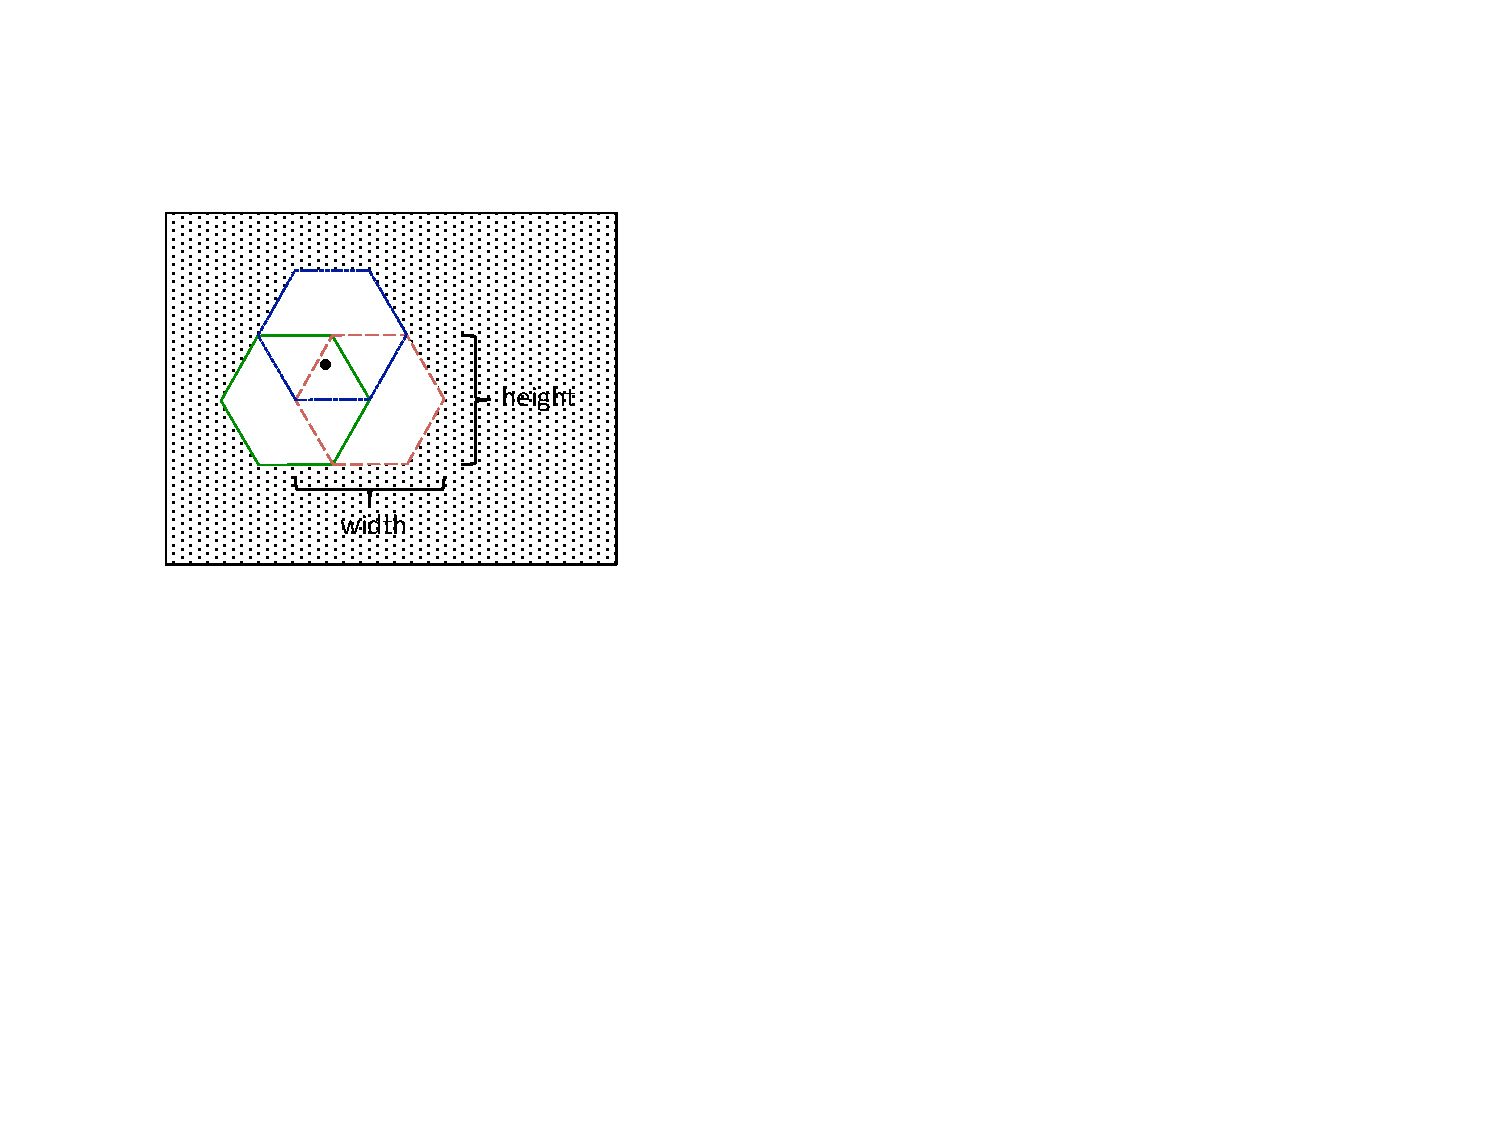
\includegraphics[width=0.2\textwidth]{figs/single_hex.pdf}
%     \caption{Representing a point and radius as three hexagons. The width and height correspond to the radius.}
%  \label{fig:grid}
%\end{figure}

%\begin{figure}
%  \centering
%     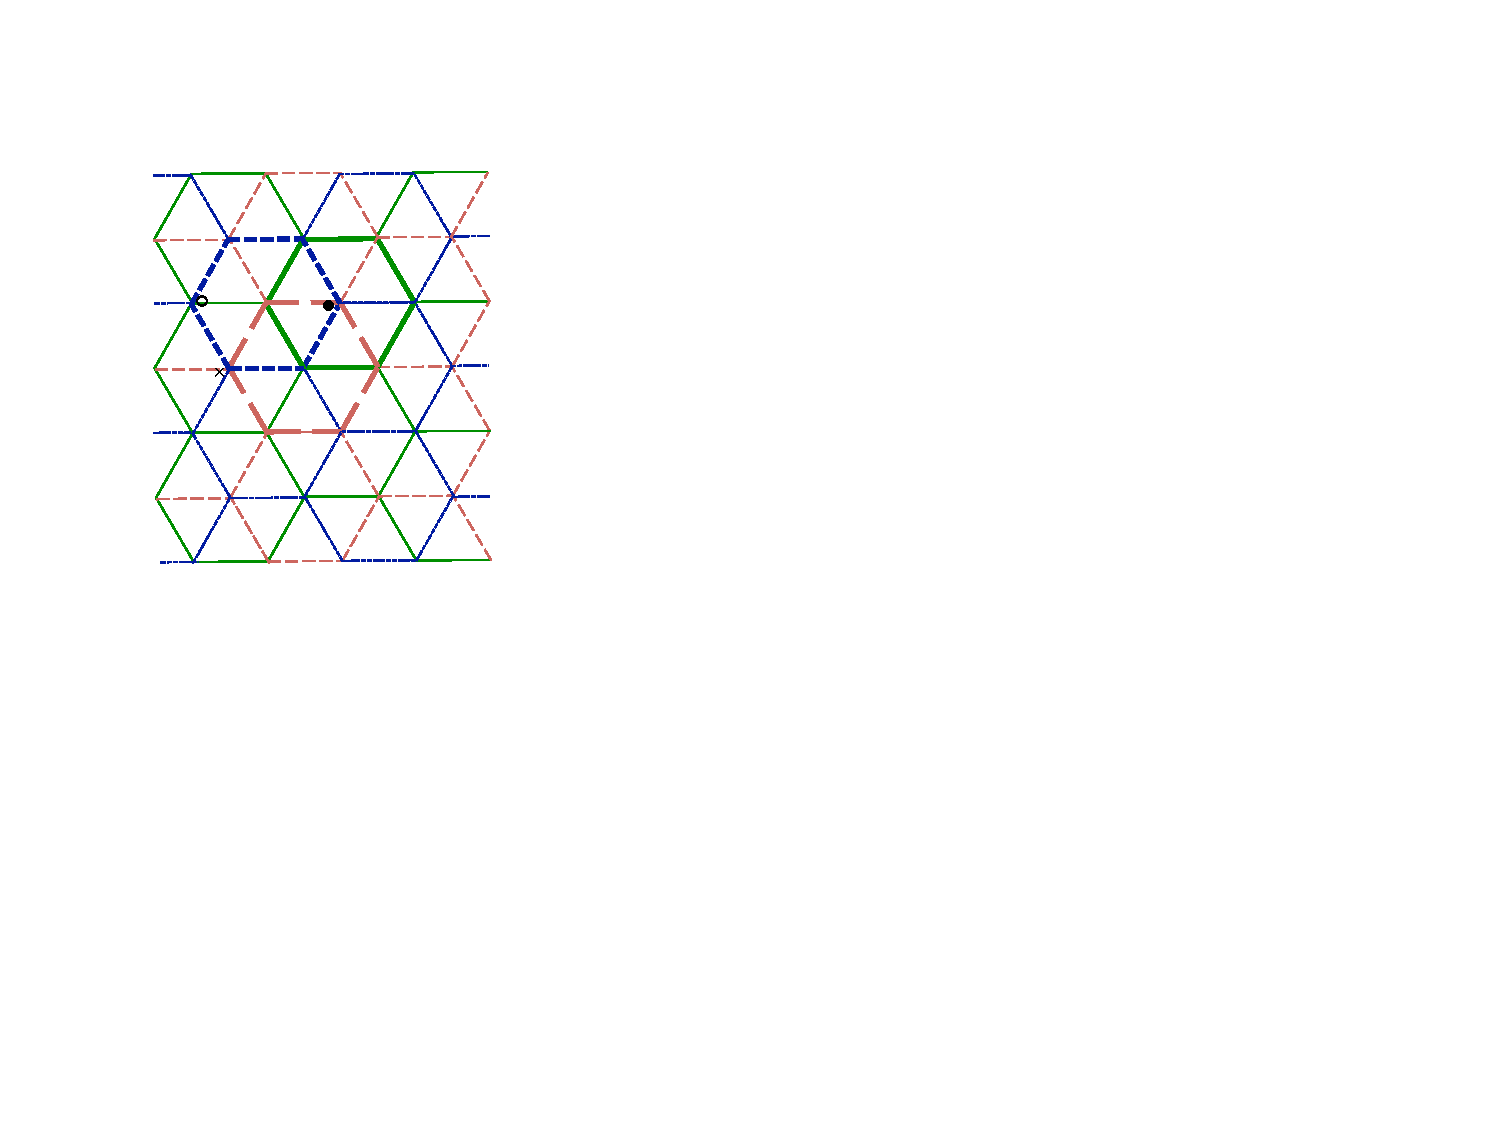
\includegraphics[width=0.25\textwidth]{figs/multiple_hex.pdf}
%     \caption{Overlay of map with multiple hexagons.}
%  \label{fig:grid2}
%\end{figure}

For this dataset, we present results for the following three queries:
\begin{verbatim}
Q1: SELECT COUNT(*) WHERE category="Thai"

Q2: SELECT TOP 10 restaurant
WHERE category="Mexican" AND
(hex2mi=1 OR hex2mi=2 OR hex2mi=3)
ORDER BY stars

Q3: SELECT restaurant, MAX(stars) 
WHERE category="Mexican" OR
category="Chinese" OR category="Indian"
OR category="Greek" OR category="Thai"
OR category="Japanese"
GROUP BY category
\end{verbatim}

Q1 is a count on the number of Thai restaurants.
%In our dataset, we map the category string to an integer id.
%The input domain is 11 bits for this query because there are 900 categories.
Q2 returns the top 10 Mexican restaurants within
a 2 mile radius of a user-specified location by querying three hexagons.
We assume that the provider caches the intermediate table for the 
Top 10 query as described in Section~\ref{sec:topk} because it is a common query.
%The query size is large because the user has to query for restaurants 
%that match one of the three location hexagons.
%The input domain is 22 bits for this query (11 bits for the category and 11 bits for 
%the hexagon id).
Finally, Q3 returns the best rated restaurant from
a subset of categories.
This requires more communication than other queries because 
it performs a MAX with many disjoint conditions, 
as described in Section~\ref{sec:min-max}. Although most queries will probably
not have this many disjoint conditions, we test this query to show
that Splinter's protocol for this case is also practical.

Note that for Q2 and Q3, the communication costs will be higher compared
to Q1 because in Q2 and Q3, 
we are returning ASCII-encoded strings of the restaurant names rather
than just an integer in Q1.

%Although the intermediate table is smaller, the FSS scheme has to process more bits.
%Finally, in this query, the slower multi-party FSS with Paillier 
%and caching previous FSS evaluations during the query are not useful
%because the intermediate table has distinct values for the predicate
%describing the category and location.

\paragraph{Flight search:}
We implement a flight search service similar to Kayak~\cite{kayak}, using 
a public flight dataset~\cite{enigma}. The columns
are flight number, origin, destination, month, delay, and price. To find a flight,
we search by origin-destination pairs. 
We present results for two queries:

\begin{verbatim}
Q1: SELECT AVG(price) WHERE month=3 
AND origin=1 AND dest=2

Q2: SELECT TOP 10 flight_no
WHERE origin=1 and dest=2 ORDER BY price
\end{verbatim}

Q1 shows the average price for a flight during a certain month.
%If we 
%issue this query for every month, we can obtain a histogram of average prices for the year.
%In this query, the input domain is 17 bits (13 bits
%for flight number and 4 bits for the month).
Q2 returns the top 10 cheapest flights for a given source and destination, which 
we encode as integers.
Since this is a common query, the results in Figure~\ref{fig:big-results} 
assume a cached Top 10 intermediate table. 
%This query
%has an input domain of 13 bits.

\paragraph{Map routing:}
We implement a private map routing service, using real traffic map data from~\cite{dimacs} for New York City.
However, implementing map routing in Splinter is difficult because the providers can
perform only a restricted set of operations. The challenge is to find a shortest path 
algorithm compatible with Splinter. Fortunately,
%Storing all possible shortest paths requires 
%substantial amounts of storage. For example, 
%storing all shortest paths for New York City requires $2^{36}$ rows! 
%The user could download the map and find the shortest path locally, which
%is bandwidth heavy, and the user would also have to download updates constantly.
extensive work has been done to optimize map routing~\cite{bast2015route}.
One algorithm compatible with Splinter is transit node routing 
(TNR)~\cite{tnr, bast2007fast}, which has been
shown to work well in practice~\cite{bast2009ultrafast}. 
In TNR, the provider divides up a map into grids, 
which contain at least one transit node, i.e. a transit node 
that is part of a "fast" path. There is also a separate table
that has the shortest paths between all pairs of transit nodes, which 
represent a smaller subset of the map. To execute a shortest path query for a given
source and destination, the user can use FSS to download the paths
in her source and destination grid. She locally finds the shortest path to the source transit node
and destination transit node. Finally, she queries the provider for the shortest path
between the two transit nodes.

We used the source code from~\cite{tnr} and identified the 1333 transit nodes. We divided the map into 5000 grids,
and calculated the shortest path for all transit node pairs. The grid table has 5000 rows
representing the edges and nodes in a grid, and the transit node table has about 800,000
rows representing the number of shortest paths for all transit node pairs. 

Figure~\ref{fig:big-results} shows the total response time for a routing query
between a source and destination in NYC. Figure~\ref{fig:map-results} shows
the breakdown of time spent on querying the grid and transit node table.
One observation is that the multi-party version is slightly faster than the two party
version because it is faster at processing the grid query as shown in Figure~\ref{fig:map-results}.
The two-party version of FSS requires using GMP operations, which is slower than integer operations
used in the multi-party version, but the two-party version requires less bandwidth.

\begin{figure}
	\centering
		\begin{tabular}{cccc}
			\toprule
			\bf FSS scheme & \bf Grid & \bf Transit Node & \bf Total \\
			\midrule
			Two Party & 0.35 s  & 0.85 s & 1.2 s \\
			Multi-party & 0.15 s & 0.85 s & 1.0 s \\
			\bottomrule
		\end{tabular}
	\caption[Grid, transit node, and total query times for NYC map.]
	{Grid, transit node, and total query times for NYC map. 
		A user issues 2 grid queries and one transit node query. The two grid queries
		are issued together in one message, so there are a total of 2 network round trips.}
	\label{fig:map-results}
\end{figure}

\paragraph{Discussion:}
Splinter has response times of 50 ms to 1.6 seconds. Although these response times are
much higher compared to a system with FSS and Splinter, 
privacy-sensitive users are often willing
to trade some performance for better security. For
example, fetching a website on Tor 
takes a couple of seconds~\cite{torStats}.
Therefore, we believe that our performance is 
acceptable.

\subsubsection{Communication Costs}
\label{sec:communication}
Figure~\ref{fig:big-results} shows the total bandwidth of a query request and response
for the various case study queries. The sum of those
two values represents total bandwidth between the providers and user.

There are two main observations. First, both the query and response sizes are \textit{much smaller} than the size
of the database in most cases. 
Second, for non-aggregate queries, the multi-party protocol has 
a smaller response size compared to the two-party protocol but the query size is much larger
than the two-party protocol, leading to higher overall communication. 
For aggregate queries, the multi-party FSS scheme is only xor homomorphic, so
it outputs all the matches for a specific predicate/condition. The user has to perform
the aggregation locally, leading to a larger response size than the two-party protocol.
Overall, the multi-party protocols have higher total bandwidth compared to the two-party protocols
despite some differences in response size. However, FSS is a relatively new cryptographic
primitive, especially compared to PIR and garbled circuits, so we believe that
improvements in the FSS protocol could 
lower these communication costs in the future.

As stated in Section~\ref{sec:splinter_cases}, querying with 
Splinter and PIR systems should be more efficient than
downloading the whole database, assuming that such a download is possible
(no rate limiting or query restrictions). To better quantify
the "break even" point, i.e. where the communication costs is equal
to the database size, we look at our case study datasets.
For Restaurant Q1 and the 2-party version of Q2, 
it would take 1000-10,000 queries before reaching that point. 
Users probably query Yelp 1-2 times a day, so it would take at least a year
to reach the break even point. As a result, it might more sense to use
Splinter as updates might occur during that time period.
For Restaurant Q3 and multi-party Q2, it would take about 10-100 queries to reach
that point. In this case, it might make sense to download the whole database, 
but improvements to FSS could lower the costs of bandwidth in the future.
For flights, it would take about 550-100,000 queries, and for maps,
it would take 2500-25,000 queries. However, these two databases are larger
than Yelp and change more frequently, so it might not make sense
to download the database.

%\subsection{Impact of caching FSS outputs}
%\label{sec:eval_cache}
%In this section, we evaluate the impact of caching FSS outputs in the same query
%as described in Section~\ref{sec:caching}. One observation is that caching
%has no effect on certain queries, such as the Top-10 and the map routing queries, because
%for the commonly queried predicate column in the table, each record has a distinct value.
%It works well for queries where the predicate column has few distinct values relative to the 
%number of records, such as the restaurant COUNT and flights AVG query described above.
%
%\begin{figure}
%\centering
%\small
%\scalebox{0.85}{
%\begin{tabular}{ccccc}
%\toprule
%\bf Query & \bf FSS scheme & \bf No caching  & \bf Caching & \bf Speedup\\
%\midrule
%\multirow{2}{*}{Restaurant Q1} & Two-Party & 271 ms & 57 ms & 4.8x \\
% & Multi-party & 252 ms & 52 ms & 4.8x\\
%\multirow{2}{*}{Flight Q2} & Two-Party & 14.6 s & 1.5 s & 9.7x \\
%& Multi-party & 50.6 s & 1.6 s & 31.6x \\
%\bottomrule
%\end{tabular}
%}
%\caption{Speed up of queries as a result of caching FSS outputs in the same query.}
%\label{fig:caching-result}
%\end{figure}
%
%Figure~\ref{fig:caching-result} shows some examples of speed ups of queries as a result
%of caching FSS outputs in the same query. For the Yelp query, there were only about 900
%unique categories, so each provider only needed to perform about 900 FSS operations on the 
%database of 225,000 rows per query. 
%For the flight query on average price for a specific flight in a month, 
%there were only about 5000 unique
%source-destination pairs, so each provider only needed to perform about 5000 FSS operations
%per query for a database with 6.1 million rows.]

\subsubsection{Coverage of Supported Queries}
\label{sec:supported_queries}

%\begin{figure}[h]
%\centering
%\scalebox{0.78}{
%\begin{tabular}{c|C{3cm}|c}
%\toprule
%\bf Website & \bf Splinter Primitive & \bf \# of Search Features \\
%\midrule
%\multirow{3}{*}{Yelp} & Equality & 4 \\
%%\midrule
% & Range & 2 \\
%%\midrule
% & Sorting & 4 \\
%\midrule
%\multirow{4}{*}{Hotels.com} & Equality & 3 \\
%%\midrule
% & Range & 3 \\
%%\midrule
% & Sorting & 4 \\
% & Not supported & 1 \\
%\midrule
%\multirow{3}{*}{Kayak} & Equality & 4 \\
%%\midrule
% & Range & 4 \\
%%\midrule
% & Not supported & 1 \\ 
%\midrule
%Google Maps & Equality & 3 \\
%\bottomrule
%\end{tabular}
%}
%\caption{Example websites and the number of search features supported by Splinter for a given primitive.}
%\label{fig:websites}
%\end{figure}


\begin{figure}
	\centering
		\begin{tabular}{c|c|c}
			\toprule
			\bf Website & \bf Search Feature & \bf Splinter Primitive \\
			\midrule
			\multirow{3}{*}{Yelp} & Booking Method, Cities, Distance & Equality \\
			%\midrule
			& Price & Range \\
			%\midrule
			& Best Match, Top Rated, Most Reviews & Sorting \\
			& Free text search & --- \\
			\midrule
			\multirow{4}{*}{Hotels.com} & Destination, Room type, Amenities & Equality \\
			%\midrule
			& Check in/out, Price, Ratings & Range \\
			%\midrule
			& Stars, Distance, Ratings, Price & Sorting \\
			%\midrule
			& Name contains & --- \\
			\midrule
			\multirow{2}{*}{Kayak} & From/To, Cabin, Passengers, Stops & Equality \\
			%\midrule
			& Date, Flight time, Layover time, Price & Range \\
			%\midrule
			\midrule
			Google Maps & From/To, Transit type, Route options & Equality \\
			\bottomrule
		\end{tabular}
	\caption{Example website search features and their equivalent Splinter query class.}
	\label{fig:websites}
\end{figure}

We also manually characterized the applicability of Splinter to several widely used online services by studying how many of the search fields on these services' interfaces Splinter can support.
Figure~\ref{fig:websites} shows the results. 
Most services use equality and range predicates: for example, the
Hotels.com user interface includes checkboxes for selecting categories, neighborhoods, stars, etc, a range fields for price, and one free-text search field that Splinter does not support.
In general, all features except free-text search could be supported by Splinter.
For free-text search, simple keywords that map to a category (e.g., ``grocery store'') could also be supported.

\subsubsection{Comparison to Other Private Query Systems}
\label{sec:comparison}

\begin{figure}
	\centering
	\begin{tabular}{lcc}
		%\multicolumn{3}{c}{Round Trips (RTs) Required}\\
		\toprule
		\bf Splinter Query & \bf RTs in~\cite{goldberg} & \bf RTs in Splinter \\
		\midrule
		Restaurant Q1 & 6 & 1 \\
		\midrule
		Restaurant Q2 & 6 & 1 \\ 
		\midrule
		Restaurant Q3 & 6 & 11 \\
		\midrule
		Flights Q1 & 13 & 1 \\
		\midrule
		Flights Q2 & 8 & 1 \\
		\midrule
		Map Routing & 19 & 2 \\
		\bottomrule
	\end{tabular}
	\caption{Round trips required in Olumofin et al.~\cite{goldberg} and Splinter.\protect\footnotemark}
	\label{fig:rt-comparison}
\end{figure}

\begin{figure}
	\centering
	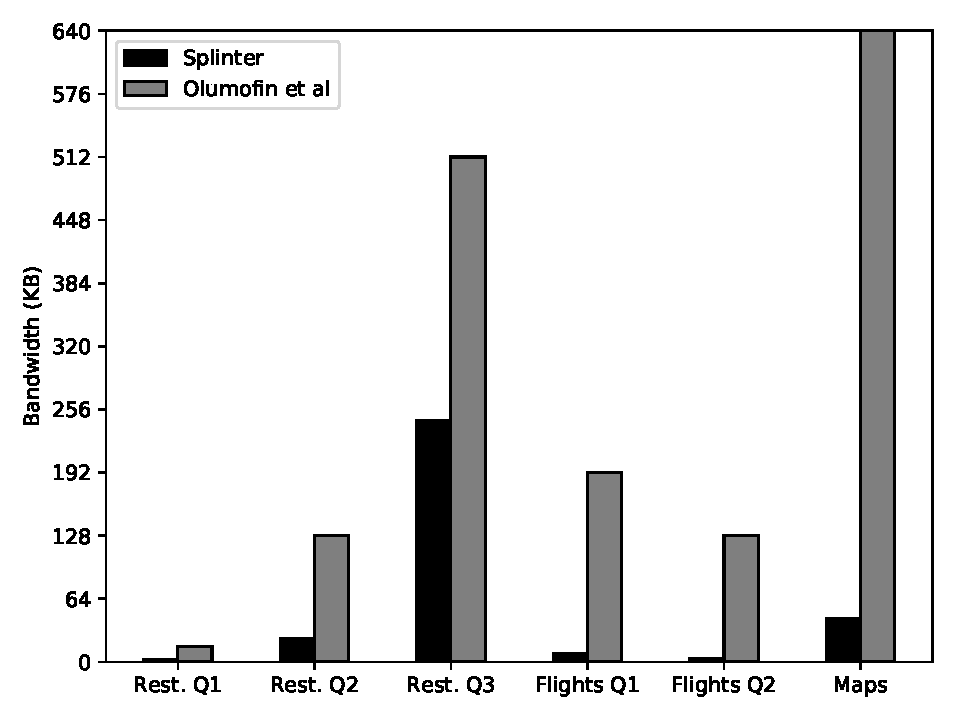
\includegraphics[width=\textwidth]{splinter-figs/bandwidth_comparison.pdf}
	\caption{Total bandwidth for Splinter and Olumofin et al.~\cite{goldberg}}
	\label{fig:bandwidth_comp}
\end{figure}

\footnotetext{
	The number of round trips in Restaurant Q3 is $O(\log n)$ in both Splinter and Olumofin et al., but the absolute number is higher in Splinter because we use a binary search whereas Olumofin et al.~use a 4-ary tree. Splinter could also use a 4-ary search to achieve the same number of round trips, but we have not yet implemented this.}

\begin{figure}
	\centering
	\begin{tabular}{lcc}
		%\multicolumn{3}{c}{Round Trips (RTs) Required}\\
		\toprule
		\bf Splinter Query & \bf Time in~\cite{goldberg} & \bf Time in Splinter \\
		\midrule
		Restaurant Q1 & 40 ms & 40 ms \\
		\midrule
		Restaurant Q2 & 135 ms & 130 ms \\ 
		\midrule
		Restaurant Q3 & 1.1 s & 1.1 s \\
		\midrule
		Flights Q1 & 10.9 s & 0.97 s \\
		\midrule
		Flights Q2 & 150 ms & 15 ms \\
		\midrule
		Map Routing & 10.6 s & 1.1 s \\
		\bottomrule
	\end{tabular}
	\caption{Server-side computation costs for Olumofin et al.~\cite{goldberg} and Splinter.}
	\label{fig:serverside-comparison}
\end{figure}

To the best of our knowledge, the most recent
private query system that can perform a similar class of queries
as Splinter is that of Olumofin et al.~\cite{goldberg},
which uses multi-party PIR. We simulate our case study queries 
on their system with similar parameters.
We compare only two-party Splinter with Olumofin et al.
because the system of Olumofin et al. assumes only two parties 
and does not describe how to handle more servers.
\footnote{From our understanding, it is possible for Olumofin et al. to support
	more than two parties, but server-side computation and bandwidth would increase
	substantially, eliminating effects of the optimizations described in their paper.}
In particular, we compare Olumofin et al. and Splinter on
the following three metrics: number of  
round trips, bandwidth, and server-side computation. 

Olumofin et al. creates
an $m$-ary ($m=4$) B+ index tree for the dataset and
uses PIR to search through
it to return various results. As a result, their queries
require $O(\log_m n)$ round trips, where $n$ is
the number of records. In Splinter, the number of rounds trips
does not depend on the size of the database for most queries.
As shown in Section~\ref{sec:min-max} and Section~\ref{sec:topk}, 
the exception is for MIN/MAX and TOPK queries with many disjoint
conditions where Splinter's
communication is similar; if there are a small number of disjoint
conditions, Splinter will be faster than previous systems 
because the user can issue parallel queries.

Figure~\ref{fig:rt-comparison} shows 
the round trips required in Olumofin et al.'s system and in Splinter
for the queries in our case studies. Splinter improves over~\cite{goldberg}
by up to an order of magnitude. Restaurant Q3
uses a disjoint MAX, so the number of round trips is similar.

Figure~\ref{fig:bandwidth_comp} shows the total bandwidth
required in Olumofin et al.'s system and in Splinter. Note that
Olumofin et al. does not have a direct way to support queries with
disjoint OR conditions used in Restaurant Q3, so we assumed that they issue a separate query
for each OR condition. Splinter has much lower overall communication
costs, especially for the queries on the larger flights and maps
databases. The main reason for this is that the bandwidth
in PIR depends on both the number of database records (specifically a square root factor) 
and record size whereas in FSS, the bandwidth depends just on the record size and is
independent of the number of records. Therefore, the disparity in bandwidth
will increase as the database size increases. This larger bandwidth
is problematic on mobile networks where data is more expensive.

Figure~\ref{fig:serverside-comparison} shows the server-side computation
costs for both systems. As expected, there is not much difference 
on the smaller restaurant database, but the difference is much larger
on the bigger databases. However, Olumofin et al. has higher round trips
for the smaller database, which increases the overall response times. For example,
in our experimental setup with 14 ms network latency, Olumofin et al. would 
incur an additional 70 ms delay versus Splinter for the restaurant queries. 
This delay increases as we move to mobile networks. If we replace
the client with a mobile device on a 4G network, the network latency
would be approximately 100 ms~\cite{mobile-delays}. Therefore,
the restaurant queries would incur an additional 500 ms delay in Olumofin et al.
compared to Splinter. For bigger databases, the number of round trips increases,
so the total amount of latency incurred will also increase. For instance,
for maps, the additional latency on Olumofin et al. would be about 1.7 seconds.

%We see a similar performance difference from the results
%in~\cite{goldberg}'s evaluation, which reports response times of
%of 2-18 seconds for queries with several million records, compared to
%50 ms to 1.6 seconds in Splinter.
%Moreover, the experiments in~\cite{goldberg} do not use a real network,
%despite having a large number 
%of round trips, so their response times would be even longer
%on high-latency networks.
Finally, the system in~\cite{goldberg} has weaker security guarantees:
it requires \textit{all} the providers to be honest, whereas Splinter
only requires that \textit{one} provider is honest. 

%For maps, a recent system by Wu et al.~\cite{wu2016} used
%garbled circuits for map routing. They achieve response times
%of 140-784 seconds for their maps with Los Angeles as their largest map,
%and require 8-16 MB of total bandwidth. Splinter has a response time of 1.2
%seconds on a larger map (NYC), which is $100\times$ lower, and with
%a total bandwidth of 45-725 KB, which is $10\times$ lower.

%\begin{figure}
%\centering
%\scalebox{0.9}{
%\begin{tabular}{lcc}
%\multicolumn{3}{c}{Bytes Transferred}\\
%\toprule
%\bf Splinter Query & \bf \cite{goldberg} & \bf Splinter \\
%\midrule
%Restaurant Q1 & 3-30 KB & 1 \\
%\midrule
%Restaurant Q2 &  & 1 \\ 
%\midrule
%Flights Q1 & 22 & 1 \\
%\midrule
%Flights Q2 & 12 & 1 \\
%\midrule
%Map Routing & 19 & 2 \\
%\bottomrule
%\end{tabular}
%}
%\caption{For the queries in our evaluation, we show the estimated difference in round trips between Olumofin et al.~\cite{goldberg} and Splinter.}
%\label{fig:comparison}
%\end{figure}


\subsubsection{FSS Microbenchmarks}
\label{sec:micro}
Cryptographic operations are the main
cost in Splinter.
We present microbenchmarks to show these costs of various
parts of the FSS protocol, 
tradeoffs between various FSS protocols,
and the throughput of FSS. The microbenchmarks
also show why the response times in Figure~\ref{fig:big-results} 
are different between the two-party and multi-party FSS cases.
All of these experiments are done on one core to show the 
per-core throughput of the FSS protocol.

\paragraph{Two-party FSS:}
For two-party FSS, generating a function share takes less than 1 ms.
The speed of FSS evaluation is proportional to the size of the input domain, i.e. number of bits per record. 
We can perform around 700,000 FSS evaluations per second on
24-bit records, i.e. process around 700,000
distinct 24-bit records, using one-way compression functions.
Figure~\ref{fig:micro2} shows the per-core throughput of our implementation
for different FSS schemes, i.e. number of unique database records that can be processed
per second. It also shows that using one-way compression functions
as described in Section~\ref{sec:fastfss}, we obtain a $2.5\times$ speedup over using 
AES as a PRG.

\begin{figure}
	\centering
	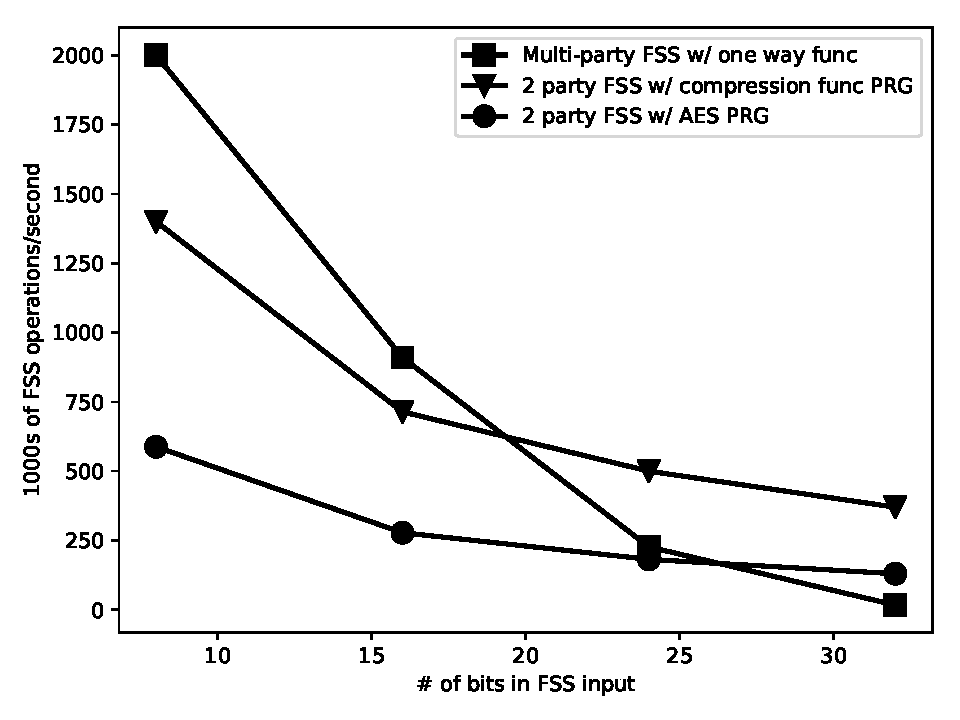
\includegraphics[width=\textwidth]{splinter-figs/micro.pdf}
	\caption[Per-core throughput of various FSS protocols.]{Per-core throughput of various FSS protocols. 
		The graph shows the number of FSS operations that can be performed, i.e. database records processed, per second for various input sizes, on one core.}
	\label{fig:micro2}
\end{figure}


\paragraph{Multi-party FSS:}
As shown in Figure~\ref{fig:micro2}, for the multi-party FSS 
scheme from~\cite{fss} that only uses one-way functions, 
the time to generate the function share and evaluate it is proportional
to $2^{n/2}$ where $n$ is the number of bits in the input domain. 
The size of the share scales with $2^{n/2}$
rather than just $n$ in the two-party case. 
An important observation is that using one-way compression 
functions instead of AES does not make a significant difference for multi-party 
FSS because the PRG is called less often compared to two-party FSS. 
For small input domains ($<$ 20 bits), 
the multi-party version of FSS is faster than the 2-party version, but 
a provider cannot aggregate locally for SUM and COUNT queries in the multi-party version.
%However, for smaller input domains, at the
%cost of additional bandwidth for increased function share size, she will receive faster execution and
%more security by being able to split her shares.

%\begin{figure}
%	\centering
%		\begin{tabular}{cC{2.7cm}C{3cm}}
%			\multicolumn{3}{c}{Time to generate function shares} \\
%			\toprule
%			\bf \# of bits & \bf Query Gen in Boyle et al~\cite{fss} & \bf Query Gen in Riposte~\cite{corrigan-gibbs:riposte}\\
%			\midrule
%			8 & $<$ 1 ms  & 0.06 s \\
%			16 & $<$ 1 ms & 1 s \\
%			24 & 44 ms & 16 s \\
%			32 & 166 ms & 265 s \\
%			\bottomrule
%		\end{tabular}
%	\caption{Query generation times for multi-party FSS schemes using one-way functions~\cite{fss} and
%		using Paillier~\cite{corrigan-gibbs:riposte}.}
%	\label{fig:mp_querygen}
%\end{figure}
%
%For the scheme from~\cite{corrigan-gibbs:riposte}, which uses Paillier encryption, generating
%a function share is slower compared to~\cite{fss} because 
%it requires many exponentiations over a large integer group and 
%depends on the number of record bits. Figure~\ref{fig:mp_querygen} 
%shows a summary of the query generation times
%for both schemes. However, the 
%evaluation of the function share is independent of the size of
%the input domain. The output of the function share in~\cite{corrigan-gibbs:riposte}
%returns a group element that is additive in a large integer group, but in
%order to have this property, the performance is lower compared to~\cite{fss}.
%We can perform 250 FSS evaluations a second, but this lower performance 
%is useful for SUM and COUNT operations on bandwidth-constrained clients.

\subsubsection{Hosting Costs}
\label{sec:pricing}
We estimate Splinter's server-side computation cost on Amazon EC2, 
where the cost of a CPU-second using Amazon Lambda is about 0.005 cents. 
The cost of storage and running a web server can be amortized over requests.
We found that most of our queries cost less than 0.005 cents. Map queries are a bit more costly,
about 0.05 cents to run a shortest path query for NYC, because the amount of 
computation required is higher. With the decreasing cost of cloud computing resources~\cite{decrease-aws},
we expect costs to become even lower over time. Although there are other costs associated with running a web service,
our results show that Splinter's server-side computation costs are very reasonable.
%Costs for Amazon AWS and other cloud services have been decreasing because
%of innovation and competition~\cite{aws-decreasing}, and further improvements to the FSS protocol
%could also reduce costs. Therefore, we expect our costs per query to decrease over time.


\subsection{Discussion and Limitations}
\label{spl-sec:discussion}

\paragraph{Economic feasibility:}
\label{sec:disc-economics}

Although it is hard to predict real-world deployment, we believe that Splinter's low cost makes it economically feasible for several types of applications.
Here are some possible methods for monetization.
For example, despite many current data owners, such as Yelp and Google Maps, generating revenue primarily by showing ads and mining user data,
they can license their data to Splinter providers and have these providers manage a Splinter deployment. The providers
can then charge a subscription fee, e.g. \$1 a month, for usage of the server.
Similarly, these providers can collectively issue a utility token that
can be used to pay for the queries.
Splinter's trust model, where only one provider needs to be honest, also makes 
it easy for new providers to join the market, increasing users' privacy.

This businesses seems reasonable as studies have shown that 
many consumers are willing to pay for services that protect their privacy~\cite{atlantic,atlantic2}. 
In fact, users might not use certain services because of privacy concerns~\cite{ravichandran2009capturing,riley2008tolls}.
Similarly, more users are using sites like DuckDuckGo and technologies like Tor 
because they are unwilling to have sites track their
query behavior, which shows a growing consumer market for privacy-preserving technologies. 
However, whether such a business model would work or be feasible 
in practice is beyond the scope of this dissertation.
%Well-known sites like OkCupid, Pandora, Youtube, and Slashdot allow users to 
%pay a monthly fee to remove ads that collect their information, showing there is
%already a demographic willing to pay for privacy. Moreover,

%As shown in Section~\ref{sec:pricing}, the cost of running queries on Splinter is low, with our most expensive query, map routing, costing less than 0.005 cents in AWS resources.
%At this cost, providers could offer Splinter-based map routing for a subscription fee of \$1 per month.
%Moreover, the availability of techniques like Splinter might make it easier to introduce 
%regulation about privacy in certain settings, similar to current privacy regulations in HIPAA~\cite{hipaa}
%and GDPR~\cite{gdpr}.

%Nonetheless, there are already successful open databases containing most of the data in these services, such as OpenStreetMap~\cite{osm}, and basic data on locations does not change rapidly once collected.
%There are already multiple Android and iOS applications that download subsets of OpenStreetMap data for  offline routing and update it periodically~\cite{osm-offline}.

%\subsection{Extensions to Splinter}
%\label{sec:disc-extensions}
%
%To support more workloads, Splinter's query model and evaluation algorithms can be extended in several ways.

%Finally, Splinter does have some limitations.
%First, FSS, like PIR, requires scanning the whole input dataset on
%every query, to prevent providers from figuring out which records have
%been accessed.
%Second, Splinter does not support some SQL features, such as private join conditions.
%Despite these limitations, we show that Splinter is practical on large
%real-world datasets, such as maps, and can support many of today's online applications.
%Because human-created datasets are unlikely to grow faster than
%hardware capabilities in the future, we believe Splinter's techniques will only
%become more practical over time.

\paragraph{Unsupported queries:}
As shown in Section~\ref{sec:querymodel}, Splinter supports only a subset of SQL.
Splinter does not support partial text matching or image matching, which are common in types of applications
that might use Splinter. Moreover, Splinter cannot support private joins, i.e. Splinter can only support joining with 
another table if the join condition is public, which encompasses a large majority of join operations. 
Despite these limitations, our study in Section~\ref{sec:supported_queries} 
shows Splinter can support many application search interfaces.

\paragraph{Number of providers:} 
One limitation of Splinter is that 
a Splinter-based service has 
to be deployed on at least two providers. 
However, previous practical PIR systems described in Section~\ref{spl-sec:related}
also require at least two providers. 

%Unlike those systems, 
%Splinter requires only \textit{one} honest provider whereas those systems
%require \textit{all} providers be honest. Moreover,
%current multi-party FSS schemes do not scale well past 
%three providers, but we believe that further research will improve its efficiency.

%\paragraph{Joins:}
%As shown in Section~\ref{sec:querymodel}, Splinter can support only joining with another table 
%if the join condition is public,
%i.e. the join condition cannot contain sensitive or private information. To do this, 
%providers can run the join before filtering the data using the private condition.
%We leave the development of private join conditions to future work.

\paragraph{Full table scans:}
FSS, like PIR, requires scanning the whole input dataset on every Splinter query,
to prevent providers from figuring out which records have been accessed. 
Despite this limitation, we have shown that Splinter is practical
on large real-world datasets, such as maps.

Splinter needs to scan the whole table only for conditions 
that contain sensitive parameters.
For example, consider the query:
\begin{verbatim}
SELECT flight from table WHERE src=SFO 
AND dst=LGA AND delay < 20
\end{verbatim}
If the user does not consider the delay of 20 in this query to be
private, Splinter could send it in the clear.
The providers can then create an intermediate
table with only flights where the delay $<$ 20 and apply the private
conditions only to records in this table.
In a similar manner, users querying geographic data may be willing to
reveal their location at the country or state level but would like to
keep their location inside the state or country private.

\paragraph{Maintaining consistent data views:}
Splinter requires that each provider executes a given user
query on the same copy of the data. 
Much research in distributed systems has focused on ensuring
databases consistency across multiple providers~\cite{spanner, ongaro:raft, tu:silo}.
Using the appropriate consistency techniques is dependent
on the application and an active area of research.
Applying those techniques in Splinter is beyond the scope
of this dissertation.


\subsection{Related Work}
\label{spl-sec:related}
Splinter is related to work in Private Information Retrieval (PIR),
garbled circuit systems, encrypted data systems, 
and Oblivious RAM (ORAM) systems. Splinter achieves higher performance than these systems 
through its mapping of database queries to the Function Secret Sharing (FSS) primitive.

\paragraph{PIR systems:}
Splinter is most closely related to systems that use Private
Information Retrieval (PIR)~\cite{chor1998private} to query a database privately.
In PIR, a user queries for the $i^\mathrm{th}$ record in the database, and the database
does not learn the queried index $i$ or the result.
Much work has been done on improving 
PIR protocols~\cite{ostrovsky2007survey, olumofin2011revisiting}. 
Work has also been done to extend PIR to return multiple records~\cite{groth2010multi},
but it is computationally expensive.
Our work is most closely related to the system in~\cite{goldberg}, which implements
a parametrized SQL-like query model similar to Splinter using PIR, but requires
more computation than Splinter.

Popcorn~\cite{popcorn} is a media delivery service that 
uses PIR to hide user consumption habits from the provider
and content distributor. However, Popcorn is optimized for
streaming media databases, like Netflix, which have a small number (about 8000)
of large records. 

The systems above have a weaker
security model: \textit{all} the providers need to be honest.
Splinter requires only \textit{one} honest provider and 
is more efficient because it 
extends Function Secret Sharing (FSS)~\cite{fss,gilboa2014distributed}, which 
enables executions of complex operations such as SUMs in one round trip
instead of only extracting one data record at a time.

\paragraph{Garbled circuits:}
Systems such as Embark~\cite{lan2016embark}, BlindBox~\cite{blindbox}, 
and private shortest path computation systems~\cite{wu2016}
use garbled circuits~\cite{Yao, goldwasser1997multi} to perform private computation
on a single untrusted server.
Even with improvements in practicality~\cite{bellare2013efficient}, these
techniques still have high computation and bandwidth costs for queries on
large datasets because a new garbled circuit has to be generated for each query.
(Reusable garbled circuits~\cite{goldwasser:sfe} are not yet practical.)
%For example, the recent map routing system by Wu et al.~\cite{wu2016} uses garbled circuits and 
%has $100\times$ higher response time and $10\times$ higher bandwidth cost
%than Splinter.

\paragraph{Encrypted data systems:}
Systems that compute on encrypted data, like 
CryptDB~\cite{popa:cryptdb}, Mylar~\cite{popa:mylar}, SPORC~\cite{feldman:sporc},
Depot~\cite{mahajan:depot}, and SUNDR~\cite{li:sundr}, all try to protect
private data against a server compromise, which is a different
problem than what Splinter tries to solve. CryptDB is most similar to Splinter 
because it allows for SQL-like queries over encrypted data. However, all
these systems protect against a single, potentially compromised server 
where the user is storing data privately, but they do not hide data access patterns. 
In contrast, Splinter hides data access patterns and a user's query parameters 
but is only designed to operate on a cleartext 
datasets that is hosted at multiple providers.


\paragraph{ORAM systems:}
Splinter is also related to systems that use Oblivious RAM~\cite{stefanov:path-oram, lorch2013shroud}. 
ORAM allows a user to read and write data on an untrusted server without
revealing her data access patterns to the server. However, ORAM cannot be easily applied
into the Splinter setting. One main requirement of ORAM is that the user
can only read data that she has written. 
In Splinter, the provider hosts a cleartext dataset, not created by any specific user, 
and many users need to access the same dataset.

\subsection{Conclusions}
\label{spl-sec:conclusion}
Splinter is a new private query system that protects sensitive parameters
in SQL-like queries while scaling to realistic applications. Splinter uses and extends a recent
cryptography primitive, Function Secret Sharing (FSS),
allowing it to achieve much better
performance compared to previous private query systems. We develop
protocols to execute complex queries
with low computation and bandwidth. As a proof of concept,
we have evaluated Splinter with three sample applications---a Yelp clone,
map routing, and flight search---and showed
that Splinter has low response times from 50 ms to 1.6 seconds with low
hosting costs.

\section{Conclusion and Future Work}
\label{chap:concl}

In this dissertation, we presented two systems, Veil and Splinter,
to minimize data leakage when a user accesses a web service. 
%Veil is the first system that allows developers to provide
%stronger private browsing semantics without browser-side
%support. Veil minimizes the amount of user data 
%that can be recovered on a shared computer after
%a user terminates her private browsing session.
%Splinter prevents sensitive information from user
%queries in a more practical manner by 
%leveraging a recent cryptographic primitive,
%function secret sharing (FSS). 
These systems have raised new interesting questions,
especially regarding the practicality of 
systems for secure multi-party computation and private queries.

Splinter leveraged
function secret sharing (FSS) to reduce the overhead associated with private queries compared to previous
work. However, open research problems still remain. For example, can private queries scale to billions
or trillions of records? Furthermore, can private queries support more expressive operators like JOINs or
NOT conditions? What are the limitations on the types of FSS can support practically?

Multi-party computation (MPC) allows participants to evaluate a common function without revealing
their respective inputs. As hospitals, governments, and corporations increasingly transition from
paper records to electronic ones, MPC-style computations represent a natural way to securely enable
cross-organization data sharing. MPC is a well-studied cryptographic solution to this problem, but its
impracticality has prevented widespread adoption. Are there ways to do MPC on more complex
computations, such as graph queries?

With the increased number of data and privacy breaches, users are becoming
more aware of the "cost" of using web services. Moreover, regulations like
GDPR are levying heavy penalties on organizations that do not build
secure mechanisms that protect user data. As a result, we will see
an increase both in users and web services that want to prevent data leakage.
We hope that the systems in this dissertation serve
as a good foundation for thinking about practical, secure mechanisms
that prevent this leakage.
%\input{relwk}
%\input{bkgrd}
%\input{chl}
%\begin{BVerbatim}[commandchars=\\\{\}]
\PY{c}{\PYZsh{} Called by Applier layer after applying log to disk.}
\PY{k}{def} \PY{n+nf}{disklog\PYZus{}truncate}\PY{p}{(}\PY{n}{txn}\PY{p}{)}\PY{p}{:}
    \PY{n}{header} \PY{o}{=} \PY{n}{disk\PYZus{}read}\PY{p}{(}\PY{n}{CommitBlock}\PY{p}{)}
    \PY{n}{header}\PY{o}{.}\PY{n}{previous\PYZus{}len} \PY{o}{=} \PY{n}{header}\PY{o}{.}\PY{n}{len}
    \PY{n}{header}\PY{o}{.}\PY{n}{len} \PY{o}{=} \PY{l+m+mi}{0}
    \PY{n}{disk\PYZus{}write}\PY{p}{(}\PY{n}{CommitBlock}\PY{p}{,} \PY{n}{header}\PY{p}{)}
    \PY{n}{disk\PYZus{}sync}\PY{p}{(}\PY{p}{)}

\PY{c}{\PYZsh{} Called by Applier layer, which guarantees that there\PYZsq{}s enough space.}
\PY{k}{def} \PY{n+nf}{disklog\PYZus{}append}\PY{p}{(}\PY{n}{txn}\PY{p}{)}\PY{p}{:}
    \PY{n}{header} \PY{o}{=} \PY{n}{disk\PYZus{}read}\PY{p}{(}\PY{n}{CommitBlock}\PY{p}{)}
    \PY{n}{write\PYZus{}packed\PYZus{}addresses}\PY{p}{(}\PY{n}{LogDescStart}\PY{p}{,} \PY{n}{header}\PY{o}{.}\PY{n}{len}\PY{p}{,} \PY{n}{txn}\PY{p}{)}
    \PY{n}{pos} \PY{o}{=} \PY{n}{LogDataStart} \PY{o}{+} \PY{n}{header}\PY{o}{.}\PY{n}{len}
    \PY{k}{for} \PY{p}{(}\PY{n}{a}\PY{p}{,} \PY{n}{v}\PY{p}{)} \PY{k}{in} \PY{n}{txn}\PY{o}{.}\PY{n}{iteritems}\PY{p}{(}\PY{p}{)}\PY{p}{:}
        \PY{n}{disk\PYZus{}write}\PY{p}{(}\PY{n}{pos}\PY{p}{,} \PY{n}{v}\PY{p}{)}
        \PY{n}{header}\PY{o}{.}\PY{n}{checksum} \PY{o}{=} \PY{n+nb}{hash}\PY{p}{(}\PY{n}{header}\PY{o}{.}\PY{n}{checksum} \PY{o}{|}\PY{o}{|} \PY{n}{a} \PY{o}{|}\PY{o}{|} \PY{n}{v}\PY{p}{)}
        \PY{n}{pos} \PY{o}{+}\PY{o}{=} \PY{l+m+mi}{1}
    \PY{n}{header}\PY{o}{.}\PY{n}{previous\PYZus{}len} \PY{o}{=} \PY{n}{header}\PY{o}{.}\PY{n}{len}
    \PY{n}{header}\PY{o}{.}\PY{n}{len} \PY{o}{=} \PY{n}{header}\PY{o}{.}\PY{n}{len} \PY{o}{+} \PY{n+nb}{len}\PY{p}{(}\PY{n}{txn}\PY{p}{)}
    \PY{n}{disk\PYZus{}write}\PY{p}{(}\PY{n}{CommitBlock}\PY{p}{,} \PY{n}{header}\PY{p}{)}
    \PY{n}{disk\PYZus{}sync}\PY{p}{(}\PY{p}{)}

\PY{k}{def} \PY{n+nf}{disklog\PYZus{}readlog}\PY{p}{(}\PY{n}{nr}\PY{p}{)}\PY{p}{:}
    \PY{n}{checksum} \PY{o}{=} \PY{n+nb}{hash}\PY{p}{(}\PY{l+m+mi}{0}\PY{p}{)}
    \PY{n}{log} \PY{o}{=} \PY{p}{[}\PY{p}{]}
    \PY{k}{for} \PY{n}{i} \PY{k}{in} \PY{n+nb}{range}\PY{p}{(}\PY{l+m+mi}{0}\PY{p}{,} \PY{n}{nr}\PY{p}{)}\PY{p}{:}
        \PY{n}{a} \PY{o}{=} \PY{n}{read\PYZus{}packed\PYZus{}address}\PY{p}{(}\PY{n}{LogDescStart}\PY{p}{,} \PY{n}{i}\PY{p}{)}
        \PY{n}{v} \PY{o}{=} \PY{n}{disk\PYZus{}read}\PY{p}{(}\PY{n}{LogDataStart} \PY{o}{+} \PY{n}{i}\PY{p}{)}
        \PY{n}{checksum} \PY{o}{=} \PY{n+nb}{hash}\PY{p}{(}\PY{n}{checksum} \PY{o}{|}\PY{o}{|} \PY{n}{a} \PY{o}{|}\PY{o}{|} \PY{n}{v}\PY{p}{)}
        \PY{n}{log}\PY{o}{.}\PY{n}{append}\PY{p}{(}\PY{p}{(}\PY{n}{a}\PY{p}{,} \PY{n}{v}\PY{p}{)}\PY{p}{)}
    \PY{k}{return} \PY{p}{(}\PY{n}{checksum}\PY{p}{,} \PY{n}{log}\PY{p}{)}

\PY{k}{def} \PY{n+nf}{disklog\PYZus{}recover}\PY{p}{(}\PY{p}{)}\PY{p}{:}
    \PY{n}{header} \PY{o}{=} \PY{n}{disk\PYZus{}read}\PY{p}{(}\PY{n}{CommitBlock}\PY{p}{)}
    \PY{p}{(}\PY{n}{checksum}\PY{p}{,} \PY{n}{log}\PY{p}{)} \PY{o}{=} \PY{n}{disklog\PYZus{}readlog}\PY{p}{(}\PY{n}{header}\PY{o}{.}\PY{n}{len}\PY{p}{)} 
    \PY{k}{if} \PY{n}{checksum} \PY{o}{!=} \PY{n}{header}\PY{o}{.}\PY{n}{checksum}\PY{p}{:}
        \PY{p}{(}\PY{n}{checksum}\PY{p}{,} \PY{n}{log}\PY{p}{)} \PY{o}{=} \PY{n}{disklog\PYZus{}readlog}\PY{p}{(}\PY{n}{header}\PY{o}{.}\PY{n}{previous\PYZus{}len}\PY{p}{)} 
        \PY{n}{header}\PY{o}{.}\PY{n}{checksum} \PY{o}{=} \PY{n}{checksum}
        \PY{n}{header}\PY{o}{.}\PY{n}{len} \PY{o}{=} \PY{n}{header}\PY{o}{.}\PY{n}{previous\PYZus{}len}
        \PY{n}{disk\PYZus{}write}\PY{p}{(}\PY{n}{CommitBlock}\PY{p}{,} \PY{n}{header}\PY{p}{)}
        \PY{n}{disk\PYZus{}sync}\PY{p}{(}\PY{p}{)}
    \PY{k}{return} \PY{n}{log}
\end{BVerbatim}

%\input{spec}
%\input{impl}
%\input{eval}
%\section{Conclusion and Future Work}
\label{chap:concl}

In this dissertation, we presented two systems, Veil and Splinter,
to minimize data leakage when a user accesses a web service. 
%Veil is the first system that allows developers to provide
%stronger private browsing semantics without browser-side
%support. Veil minimizes the amount of user data 
%that can be recovered on a shared computer after
%a user terminates her private browsing session.
%Splinter prevents sensitive information from user
%queries in a more practical manner by 
%leveraging a recent cryptographic primitive,
%function secret sharing (FSS). 
These systems have raised new interesting questions,
especially regarding the practicality of 
systems for secure multi-party computation and private queries.

Splinter leveraged
function secret sharing (FSS) to reduce the overhead associated with private queries compared to previous
work. However, open research problems still remain. For example, can private queries scale to billions
or trillions of records? Furthermore, can private queries support more expressive operators like JOINs or
NOT conditions? What are the limitations on the types of FSS can support practically?

Multi-party computation (MPC) allows participants to evaluate a common function without revealing
their respective inputs. As hospitals, governments, and corporations increasingly transition from
paper records to electronic ones, MPC-style computations represent a natural way to securely enable
cross-organization data sharing. MPC is a well-studied cryptographic solution to this problem, but its
impracticality has prevented widespread adoption. Are there ways to do MPC on more complex
computations, such as graph queries?

With the increased number of data and privacy breaches, users are becoming
more aware of the "cost" of using web services. Moreover, regulations like
GDPR are levying heavy penalties on organizations that do not build
secure mechanisms that protect user data. As a result, we will see
an increase both in users and web services that want to prevent data leakage.
We hope that the systems in this dissertation serve
as a good foundation for thinking about practical, secure mechanisms
that prevent this leakage.

{
\begin{singlespace}
% Since we're using natbib in numbers mode, we don't need plainnat,
% which exists to feed authors and years back in to natbib.  As a
% result, it complains about entries without years, which we don't
% care about.
%\bibliographystyle{plainnat}
\bibliographystyle{plain}
\bibliography{n-str,p,n,n-conf}
\end{singlespace}
}

\end{document}
